% Options for packages loaded elsewhere
\PassOptionsToPackage{unicode}{hyperref}
\PassOptionsToPackage{hyphens}{url}
%
\documentclass[
]{article}
\usepackage{lmodern}
\usepackage{amsmath}
\usepackage{ifxetex,ifluatex}
\ifnum 0\ifxetex 1\fi\ifluatex 1\fi=0 % if pdftex
  \usepackage[T1]{fontenc}
  \usepackage[utf8]{inputenc}
  \usepackage{textcomp} % provide euro and other symbols
  \usepackage{amssymb}
\else % if luatex or xetex
  \usepackage{unicode-math}
  \defaultfontfeatures{Scale=MatchLowercase}
  \defaultfontfeatures[\rmfamily]{Ligatures=TeX,Scale=1}
\fi
% Use upquote if available, for straight quotes in verbatim environments
\IfFileExists{upquote.sty}{\usepackage{upquote}}{}
\IfFileExists{microtype.sty}{% use microtype if available
  \usepackage[]{microtype}
  \UseMicrotypeSet[protrusion]{basicmath} % disable protrusion for tt fonts
}{}
\makeatletter
\@ifundefined{KOMAClassName}{% if non-KOMA class
  \IfFileExists{parskip.sty}{%
    \usepackage{parskip}
  }{% else
    \setlength{\parindent}{0pt}
    \setlength{\parskip}{6pt plus 2pt minus 1pt}}
}{% if KOMA class
  \KOMAoptions{parskip=half}}
\makeatother
\usepackage{xcolor}
\IfFileExists{xurl.sty}{\usepackage{xurl}}{} % add URL line breaks if available
\IfFileExists{bookmark.sty}{\usepackage{bookmark}}{\usepackage{hyperref}}
\hypersetup{
  hidelinks,
  pdfcreator={LaTeX via pandoc}}
\urlstyle{same} % disable monospaced font for URLs
\usepackage{color}
\usepackage{fancyvrb}
\newcommand{\VerbBar}{|}
\newcommand{\VERB}{\Verb[commandchars=\\\{\}]}
\DefineVerbatimEnvironment{Highlighting}{Verbatim}{commandchars=\\\{\}}
% Add ',fontsize=\small' for more characters per line
\newenvironment{Shaded}{}{}
\newcommand{\AlertTok}[1]{\textcolor[rgb]{1.00,0.00,0.00}{\textbf{#1}}}
\newcommand{\AnnotationTok}[1]{\textcolor[rgb]{0.38,0.63,0.69}{\textbf{\textit{#1}}}}
\newcommand{\AttributeTok}[1]{\textcolor[rgb]{0.49,0.56,0.16}{#1}}
\newcommand{\BaseNTok}[1]{\textcolor[rgb]{0.25,0.63,0.44}{#1}}
\newcommand{\BuiltInTok}[1]{#1}
\newcommand{\CharTok}[1]{\textcolor[rgb]{0.25,0.44,0.63}{#1}}
\newcommand{\CommentTok}[1]{\textcolor[rgb]{0.38,0.63,0.69}{\textit{#1}}}
\newcommand{\CommentVarTok}[1]{\textcolor[rgb]{0.38,0.63,0.69}{\textbf{\textit{#1}}}}
\newcommand{\ConstantTok}[1]{\textcolor[rgb]{0.53,0.00,0.00}{#1}}
\newcommand{\ControlFlowTok}[1]{\textcolor[rgb]{0.00,0.44,0.13}{\textbf{#1}}}
\newcommand{\DataTypeTok}[1]{\textcolor[rgb]{0.56,0.13,0.00}{#1}}
\newcommand{\DecValTok}[1]{\textcolor[rgb]{0.25,0.63,0.44}{#1}}
\newcommand{\DocumentationTok}[1]{\textcolor[rgb]{0.73,0.13,0.13}{\textit{#1}}}
\newcommand{\ErrorTok}[1]{\textcolor[rgb]{1.00,0.00,0.00}{\textbf{#1}}}
\newcommand{\ExtensionTok}[1]{#1}
\newcommand{\FloatTok}[1]{\textcolor[rgb]{0.25,0.63,0.44}{#1}}
\newcommand{\FunctionTok}[1]{\textcolor[rgb]{0.02,0.16,0.49}{#1}}
\newcommand{\ImportTok}[1]{#1}
\newcommand{\InformationTok}[1]{\textcolor[rgb]{0.38,0.63,0.69}{\textbf{\textit{#1}}}}
\newcommand{\KeywordTok}[1]{\textcolor[rgb]{0.00,0.44,0.13}{\textbf{#1}}}
\newcommand{\NormalTok}[1]{#1}
\newcommand{\OperatorTok}[1]{\textcolor[rgb]{0.40,0.40,0.40}{#1}}
\newcommand{\OtherTok}[1]{\textcolor[rgb]{0.00,0.44,0.13}{#1}}
\newcommand{\PreprocessorTok}[1]{\textcolor[rgb]{0.74,0.48,0.00}{#1}}
\newcommand{\RegionMarkerTok}[1]{#1}
\newcommand{\SpecialCharTok}[1]{\textcolor[rgb]{0.25,0.44,0.63}{#1}}
\newcommand{\SpecialStringTok}[1]{\textcolor[rgb]{0.73,0.40,0.53}{#1}}
\newcommand{\StringTok}[1]{\textcolor[rgb]{0.25,0.44,0.63}{#1}}
\newcommand{\VariableTok}[1]{\textcolor[rgb]{0.10,0.09,0.49}{#1}}
\newcommand{\VerbatimStringTok}[1]{\textcolor[rgb]{0.25,0.44,0.63}{#1}}
\newcommand{\WarningTok}[1]{\textcolor[rgb]{0.38,0.63,0.69}{\textbf{\textit{#1}}}}
\usepackage{graphicx}
\makeatletter
\def\maxwidth{\ifdim\Gin@nat@width>\linewidth\linewidth\else\Gin@nat@width\fi}
\def\maxheight{\ifdim\Gin@nat@height>\textheight\textheight\else\Gin@nat@height\fi}
\makeatother
% Scale images if necessary, so that they will not overflow the page
% margins by default, and it is still possible to overwrite the defaults
% using explicit options in \includegraphics[width, height, ...]{}
\setkeys{Gin}{width=\maxwidth,height=\maxheight,keepaspectratio}
% Set default figure placement to htbp
\makeatletter
\def\fps@figure{htbp}
\makeatother
\setlength{\emergencystretch}{3em} % prevent overfull lines
\providecommand{\tightlist}{%
  \setlength{\itemsep}{0pt}\setlength{\parskip}{0pt}}
\setcounter{secnumdepth}{-\maxdimen} % remove section numbering
\usepackage{pmboxdraw}
\usepackage{fontspec}
\setmonofont{Menlo}[]
\usepackage{fancyvrb}[]
\fvset{samepage=true, baselinestretch=1, frame=lines}
\renewcommand{\baselinestretch}{1.2}
\ifluatex
  \usepackage{selnolig}  % disable illegal ligatures
\fi

\author{}
\date{}

\begin{document}

\title{Exploring the uses of Quantitative Types}
\author{Andre Videla}
\maketitle

\hypertarget{abstract}{%
\section{Abstract}\label{abstract}}

Idris2 is a programming language featuring Quantitative type theory, a
Type Theory centered around tracking \emph{usage quantities} in addition
to dependent types. This is the result of more than 30 years of
development spawned by the work of Girard on Linear logic. Until
recently, our understanding of linear types and their uses in
dependently-typed programs was hypothetical. However this changes with
Idris2, which allow us to explore the semantics of running programs
using linear and dependent types. In this thesis I explore multiple
facets of programming through the lens of quantitative programming, from
ergonomics, to performance. I will present how quantitative annotations
can help the programmer write program that precisely match their
intention, provide more information to the compiler better analyse the
program written, and enable the output bytecode to run faster.

\newpage
\setcounter{secnumdepth}{2}
\tableofcontents
\newpage

\hypertarget{introduction}{%
\section{Introduction}\label{introduction}}

In this project I will demonstrate different uses and results stemming
from a programming practice that allows us to specify how many times
each variable is being used. This information is part of the type
system, in our case we are tracking if a variable is allowed to be used
exactly once, or if it has no restrictions. Such types system is called
a ``linear type system''.

As we will see, there is a lot more to this story, so as part of this
thesis, I will spend some time introducing dependent types as well as
our host language: Idris. This warm up will be followed by a context
review outlining the existing body of work about linear types and
related topics. Once both the theoretical and technical landscape have
been set I will introduce the concept of linear and quantitative type.
Those two concepts together are the key to understanding the rest of
this thesis which is about the ergonomics of Quantitative Type
Theory\cite{qtt}\cite{nuttin} (QTT, for short) for software development
and the performance improvement we can derive from the linearity
features of Idris2.

The main goal of this thesis is to explore the uses of quantitative
types in a dependently-typed setting for real-world programs, those last
two chapters are the result of such exploration. With it, I aim to
explain the limitation of quantitative types and propose ways of getting
around them. Some of those ideas have been implemented in the Idris2
compiler and we discuss their details and consequences.

Let us begin slowly and introduce the basic concepts. The following will
only make assumptions about basic understanding of imperative and
functional programming.

\hypertarget{some-vocabulary-and-jargon}{%
\subsection{Some vocabulary and
jargon}\label{some-vocabulary-and-jargon}}

Technical papers are often hard to approach for the uninitiated because
of their heavy use of unfamiliar vocabulary and domain-specific jargon.
While jargon is useful for referencing complicated ideas succinctly, it
is a double edged sword as it also tends to hinder learning by obscuring
important concepts. Unfortunately, I do not have a solution for this
problem, but I hope this section will help mitigate this feeling of
helplessness when sentences seem to be composed of randomly generated
sequences of letters rather than legitimate words.

You will find more complete definitions at the end, in the glossary.

\hypertarget{type}{%
\subparagraph{Type}\label{type}}

A label associated to a collection of values. For example
\texttt{String} is the type given to strings of characters for text.
\texttt{Int} is the type given to integer values. \texttt{Nat} is the
type given to natural numbers.

\hypertarget{type-system}{%
\subparagraph{Type-System}\label{type-system}}

Set of rules the types in a program have to follow in order to be
accepted by the compiler. The goal of the type-system is to catch some
classes of errors while helping the programmer reach their goal more
easily.

\hypertarget{linear-types}{%
\subparagraph{Linear types}\label{linear-types}}

Types that have a usage restriction. Typically, a value labelled with a
linear type can only be used once, no less, no more.

\hypertarget{linearity-quantity-multiplicity}{%
\subparagraph{Linearity / Quantity /
Multiplicity}\label{linearity-quantity-multiplicity}}

Used interchangeably most of the time. They refer the the number of
times a variable is expected to be used.

\hypertarget{syntax}{%
\subparagraph{Syntax}\label{syntax}}

The structure of some piece of information, usual in the form of
\emph{text}. Syntax itself does not convey any meaning.

\hypertarget{semantics}{%
\subparagraph{Semantics}\label{semantics}}

The meaning associated to a piece of data, most often related to syntax.

\hypertarget{pattern-matching}{%
\subparagraph{Pattern matching}\label{pattern-matching}}

Destructuring a value into its constituent parts in order to access them
or understand what kind of value we are dealing with.

\hypertarget{generic-type-polymorphic-type-type-parameter}{%
\subparagraph{Generic type / Polymorphic type / Type
parameter}\label{generic-type-polymorphic-type-type-parameter}}

A type that needs a concrete type in order to be complete. For example
\texttt{Maybe\ a} takes the single type \texttt{a} as parameter. Once we
pass it the type \texttt{Int} it become the complete type
\texttt{Maybe\ Int}.

\hypertarget{programming-recap}{%
\subsection{Programming recap}\label{programming-recap}}

If you know about programming, you've probably heard about types and
functions. Types are ways to classify values that the computer
manipulates and functions are instructions that describe how those
values are changed.

In \emph{imperative programming} functions can perform powerful
operations like ``malloc'' and ``free'' for memory management or make
network requests through the internet. While powerful in a practical
sense, those functions are really hard to study because they are hard to
define in a mathematical way. In order to make life easier we only
consider functions in the \emph{mathematical} sense of the word : A
function is something that takes an input and returns an output.

\begin{Shaded}
\begin{Highlighting}[]
\NormalTok{f }\OperatorTok{:} \DataTypeTok{A} \OtherTok{{-}\textgreater{}} \DataTypeTok{B}
\end{Highlighting}
\end{Shaded}

This notation tells us what type the function is ready to ingest as
input and what type is expected as the output.

\begin{Shaded}
\begin{Highlighting}[]
\NormalTok{input    output}
\NormalTok{    v    v}
\NormalTok{f }\OperatorTok{:} \DataTypeTok{A} \OtherTok{{-}\textgreater{}} \DataTypeTok{B}
\OperatorTok{\^{}}
\NormalTok{name }
\end{Highlighting}
\end{Shaded}

This simplifies our model because it forbids the complexity related to
complex operations like arbitrary memory modification or network access
\footnote{We can recover those features by using patterns like ``monad''
  but it is not the topic of this brief introduction.}. Functional
programming describes a programming practice centered around the use of
such functions. In addition, traditional functional programming
languages have a strong emphasis on their type system which allows the
types to describe the structure of the values very precisely.

During the rest of this thesis we are going to talk about Idris2, a
purely functional programming language featuring Quantitiative Type
Theory (QTT), a type theory\footnote{\emph{Type theory} is the abstract
  study of type systems, most often in the context of pure,
  mathematical, logic. When we say ``a Type Theory'' we mean a specific
  set of logical rules that can be implemented into a \emph{Type
  System}.} based around managing resources. But before we talk about
QTT itself, we have to explain what is Idris and what are dependent
types.

\hypertarget{idris-and-dependent-types}{%
\subsection{Idris and dependent types}\label{idris-and-dependent-types}}

Before we jump into Idris2, allow me to introduce Idris\cite{idris1},
its predecessor. Idris is a programming language featuring dependent
types.

A way to understand dependent types is to think of the programming
language as having \emph{first class types}, that is, types are values,
just like any other in the language. Types being normal values means we
can create them, pass them as arguments to functions and return them
from functions. This also means the difference between ``type-level''
and ``term-level'' is blurred.

\hypertarget{simple-example}{%
\subsubsection{Simple example}\label{simple-example}}

Let us start with a very simple example of a function in Idris, without
dependent types. This function returns whether or not a list\footnote{A
  list is defined as

  ``data List a = Nil \textbar{} Cons a (List a)

  Which mean a list is either empty (\texttt{Nil}) or non-empty
  (\texttt{Cons}) and will contain an element of type \texttt{a} and a
  reference to the tail of the list, which itself might be empty or not.
  It is customary to write the \texttt{Cons} case as \texttt{::}, and in
  fact the official implementation uses the symbol \texttt{::} instead
  of the word \texttt{Cons}. It is also customary to represent the empty
  list by \texttt{{[}{]}}.} is empty:

\begin{Shaded}
\begin{Highlighting}[]
\NormalTok{isEmpty }\OperatorTok{:} \DataTypeTok{List}\NormalTok{ a }\OtherTok{{-}\textgreater{}} \DataTypeTok{Bool}
\NormalTok{isEmpty [] }\OtherTok{=} \DataTypeTok{True}
\NormalTok{isEmpty (}\OtherTok{x ::}\NormalTok{ xs) }\OtherTok{=} \DataTypeTok{False}
\end{Highlighting}
\end{Shaded}

Every Idris function is comprised of two parts, the \emph{Type
signature} and the \emph{implementation} (or body) of the function. Let
us start by dissecting the Type signature:

\begin{Shaded}
\begin{Highlighting}[]
\CommentTok{{-}{-}    ┌ Name of the function}
\CommentTok{{-}{-}    │ }
\CommentTok{{-}{-}    │         ┌ Type of the argument }
\CommentTok{{-}{-}    │         │ }
\CommentTok{{-}{-}    │         │       ┌ Return type            }
\CommentTok{{-}{-} ╭──┴──╮   ╭──┴──╮  ╭─┴──╮}
\NormalTok{   isEmpty }\OperatorTok{:} \DataTypeTok{List}\NormalTok{ a }\OtherTok{{-}\textgreater{}} \DataTypeTok{Bool}
\CommentTok{{-}{-}                ▲}
\CommentTok{{-}{-}                │ }
\CommentTok{{-}{-}                └Type parameter}
\end{Highlighting}
\end{Shaded}

Every signature starts with a name, followed by a colon \texttt{:} and
ends with a type. In this case, the type is
\texttt{List\ a\ -\textgreater{}\ Bool} which represents a function that
takes a list of \texttt{a} and returns a \texttt{Bool}. Interestingly,
the type \texttt{a} is a \emph{Type parameter} and could be anything,
this function will work for all lists, irrespective of their content.

As for the body, here is how it is composed:

\begin{Shaded}
\begin{Highlighting}[]
\CommentTok{{-}{-}    ┌ Recall the function name}
\CommentTok{{-}{-}    │   }
\CommentTok{{-}{-}    │     ┌ Pattern matching on the empty list}
\CommentTok{{-}{-}    │     │   }
\CommentTok{{-}{-}    │     │    ┌ Return value}
\CommentTok{{-}{-} ╭──┴──╮  ▼  ╭─┴──╮}
\NormalTok{   isEmpty [] }\OtherTok{=} \DataTypeTok{True}
\CommentTok{{-}{-}             ┌ Pattern matching on the non{-}empty list}
\CommentTok{{-}{-}         ╭───┴───╮}
\NormalTok{   isEmpty (}\OtherTok{x ::}\NormalTok{ xs) }\OtherTok{=} \DataTypeTok{False}
\CommentTok{{-}{-}          ▲    ▲     ╰─┬─╯}
\CommentTok{{-}{-}          │    │       └ Return value}
\CommentTok{{-}{-}          │    │}
\CommentTok{{-}{-}          │    └ Tail of the list}
\CommentTok{{-}{-}          │}
\CommentTok{{-}{-}          └ Head of the list}
\end{Highlighting}
\end{Shaded}

Function bodies are implemented with \emph{clauses} of the form
\texttt{*function\ name*\ *arguments*\ =\ *value*}, everything before
the \texttt{=} is called \emph{the left hand side} and everything after
is called \emph{the right hand side}. Arguments on the left hand side
are pattern matched, and for each corresponding match the function
return a suitable value.

In this example, we only have two cases, the empty list \texttt{{[}{]}}
and the non-empty list \texttt{x\ ::\ xs}. When we match on a value we
may discover that we can access new variables and we give them names (or
\emph{bind} them). In this case the \texttt{::} case allows us to
bind\footnote{Binding a variable means to associate a value to a
  variable. A Binder is the piece of syntax that achieves the
  association.\texttt{let\ n\ =\ 3\ in\ \ldots{}} \emph{binds} the value
  \texttt{3} to the name \texttt{n}.} the head and the tail of the list
to the names \texttt{x} and \texttt{xs}. Depending on whether we are
dealing with an empty list or not we return \texttt{True} or
\texttt{False} to indicate if the list is empty.

Pattern matching is particularly important in Idris because it allows
the compiler to better understand how the types flow through our
program. We are going to see an example of how dependent pattern
matching\cite{view_from_the_left} manifests itself when we introduce
\emph{type holes}.

\hypertarget{dependent-types-example}{%
\subsubsection{Dependent types example}\label{dependent-types-example}}

Now let us look at an example with dependent types.

\begin{Shaded}
\begin{Highlighting}[]
\NormalTok{intOrString }\OperatorTok{:}\NormalTok{ (b }\OperatorTok{:} \DataTypeTok{Bool}\NormalTok{) }\OtherTok{{-}\textgreater{}} \KeywordTok{if}\NormalTok{ b }\KeywordTok{then} \DataTypeTok{Int} \KeywordTok{else} \DataTypeTok{String}
\NormalTok{intOrString }\DataTypeTok{True} \OtherTok{=} \DecValTok{404}
\NormalTok{intOrString }\DataTypeTok{False} \OtherTok{=} \StringTok{"we got a string"}
\end{Highlighting}
\end{Shaded}

This short snippet already shows a lot of things, but again the most
important part is the type signature. Let us inspect it:

\begin{Shaded}
\begin{Highlighting}[]
\CommentTok{{-}{-}             ┌ Name of the argument}
\CommentTok{{-}{-}             │}
\CommentTok{{-}{-}             │    ┌ Type of the argument  }
\CommentTok{{-}{-}             │    │ }
\CommentTok{{-}{-}             │    │                  ┌ Return type}
\CommentTok{{-}{-}             ▼    ▼       ╭──────────┴────────────╮  }
\NormalTok{intOrString }\OperatorTok{:}\NormalTok{ (b }\OperatorTok{:} \DataTypeTok{Bool}\NormalTok{) }\OtherTok{{-}\textgreater{}} \KeywordTok{if}\NormalTok{ b }\KeywordTok{then} \DataTypeTok{Int} \KeywordTok{else} \DataTypeTok{String}
\CommentTok{{-}{-}             │               ▲}
\CommentTok{{-}{-}             └─[dependency]──┘}
\end{Highlighting}
\end{Shaded}

As you can see the return type is a \emph{program in and of itself}!
\texttt{if\ b\ then\ Int\ else\ String} returns \texttt{Int} if
\texttt{b} is \texttt{True} and \texttt{String} otherwise. Which means
the return type is different depending on the value of \texttt{b}. This
dependency is why they are called \emph{dependent types}.

\emph{Pattern matching} on the argument allows us to return different
values for each branch of our program

\begin{Shaded}
\begin{Highlighting}[]
\CommentTok{{-}{-}           ┌ \textasciigrave{}b\textasciigrave{} is True so we expect to return \textasciigrave{}Int\textasciigrave{}}
\CommentTok{{-}{-}           │}
\CommentTok{{-}{-}           │      ┌ An Int as a return value}
\CommentTok{{-}{-}           ▼    ╭─┴─╮}
\NormalTok{intOrString }\DataTypeTok{True} \OtherTok{=} \DecValTok{404} 
\NormalTok{intOrString }\DataTypeTok{False} \OtherTok{=} \StringTok{"we got a string"}
\CommentTok{{-}{-}           ▲      ╰───────┬───────╯}
\CommentTok{{-}{-}           │              └ A String as a return value}
\CommentTok{{-}{-}           │}
\CommentTok{{-}{-}           └ \textasciigrave{}b\textasciigrave{} is \textasciigrave{}False\textasciigrave{} so we expect to return a String}
\end{Highlighting}
\end{Shaded}

This typically cannot be done in programming languages with conventional
type systems. Which is why one might want to use Idris rather than Java,
C or even Haskell in order to implement their programs. Some programming
languages can exhibits some behaviours similar to dependent types but
achieving this often comes at the expense of readability, performance
and ergonomics\cite{hasochism}.

\hypertarget{holes-in-idris}{%
\subsubsection{Holes in Idris}\label{holes-in-idris}}

A very useful feature of Idris is \emph{type holes}, one can replace any
term by a variable name prefixed by a question mark, like this :
\texttt{?hole} . This tells the compiler to infer the type at this
position and report it to the user in order to better understand what
value could possibly fit the expected type. In addition, the compiler
will also report what it knows about the surrounding context to give
additional insight.

If we take our example of \texttt{intOrString} and replace the
implementation by a hole we have the following:

\begin{Shaded}
\begin{Highlighting}[]
\NormalTok{intOrString }\OperatorTok{:}\NormalTok{ (b }\OperatorTok{:} \DataTypeTok{Bool}\NormalTok{) }\OtherTok{{-}\textgreater{}} \KeywordTok{if}\NormalTok{ b }\KeywordTok{then} \DataTypeTok{Int} \KeywordTok{else} \DataTypeTok{String}
\NormalTok{intOrString b }\OtherTok{=} \OperatorTok{?}\NormalTok{hole}
\end{Highlighting}
\end{Shaded}

We can then ask the compiler what is the expected type, information
provided by the compiler will be shown with a column of
\texttt{\textgreater{}} on the left side to distinguish it from code.
When the compiler tells us about holes, its will display the variables
available in the immediate scope of the hole above a horizontal bar, and
the ``goal'' under the horizontal bar. Here is the type we get when
asking about our \texttt{hole}:

\begin{Shaded}
\begin{Highlighting}[]
\OperatorTok{\textgreater{}}\NormalTok{ b }\OperatorTok{:} \DataTypeTok{Bool}
\OperatorTok{\textgreater{}} \CommentTok{{-}{-}{-}{-}{-}{-}{-}{-}{-}{-}{-}{-}{-}{-}{-}{-}{-}{-}{-}{-}{-}{-}{-}{-}{-}{-}{-}{-}{-}{-}{-}{-}}
\OperatorTok{\textgreater{}}\NormalTok{ hole }\OperatorTok{:} \KeywordTok{if}\NormalTok{ b }\KeywordTok{then} \DataTypeTok{Int} \KeywordTok{else} \DataTypeTok{String}
\end{Highlighting}
\end{Shaded}

This information does not tell us what value we can use, however it
informs us that the return type \emph{depends on the value of
\texttt{b}} . Therefore, pattern matching on \texttt{b} might give us
more insight. It is worth noting that Idris has an interactive mode that
allows the pattern matching to be done automatically by hitting a simple
key stroke which will generate the code in the snippet automatically.
This won't be showcased here, as it is not an Idris development
tutorial, but this approach has already been put to use and proven
effective in other programming languages with proof-assistant
features\cite{tdd}\cite{agda_interactive}. Back to the example:

\begin{Shaded}
\begin{Highlighting}[]
\NormalTok{intOrString }\OperatorTok{:}\NormalTok{ (b }\OperatorTok{:} \DataTypeTok{Bool}\NormalTok{) }\OtherTok{{-}\textgreater{}} \KeywordTok{if}\NormalTok{ b }\KeywordTok{then} \DataTypeTok{Int} \KeywordTok{else} \DataTypeTok{String}
\NormalTok{intOrString }\DataTypeTok{True} \OtherTok{=} \OperatorTok{?}\NormalTok{hole1}
\NormalTok{intOrString }\DataTypeTok{False} \OtherTok{=} \OperatorTok{?}\NormalTok{hole2}
\end{Highlighting}
\end{Shaded}

Asking again what is in \texttt{hole1} gets us:

\begin{Shaded}
\begin{Highlighting}[]
\OperatorTok{\textgreater{}}\NormalTok{ hole1 }\OperatorTok{:} \DataTypeTok{Int}
\end{Highlighting}
\end{Shaded}

And \texttt{hole2} gets us:

\begin{Shaded}
\begin{Highlighting}[]
\OperatorTok{\textgreater{}}\NormalTok{ hole2 }\OperatorTok{:} \DataTypeTok{String}
\end{Highlighting}
\end{Shaded}

Which we can fill with literal values like \texttt{123} or
\texttt{"good\ afternoon"}. The complete program would look like this:

\begin{Shaded}
\begin{Highlighting}[]
\NormalTok{intOrString }\OperatorTok{:}\NormalTok{ (b }\OperatorTok{:} \DataTypeTok{Bool}\NormalTok{) }\OtherTok{{-}\textgreater{}} \KeywordTok{if}\NormalTok{ b }\KeywordTok{then} \DataTypeTok{Int} \KeywordTok{else} \DataTypeTok{String}
\NormalTok{intOrString }\DataTypeTok{True} \OtherTok{=} \DecValTok{123}
\NormalTok{intOrString }\DataTypeTok{False} \OtherTok{=} \StringTok{"good afternoon"}
\end{Highlighting}
\end{Shaded}

\hypertarget{whats-wrong-with-non-dependent-types}{%
\subsubsection{What's wrong with non-dependent
types?}\label{whats-wrong-with-non-dependent-types}}

Non-dependent type systems cannot represent the behaviour described by
\texttt{intOrString} and have to resort to patterns like \texttt{Either}
\footnote{Defined as : ``data Either a b = Left a \textbar{} Right b} to
encapsulate the two possible cases our program can encounter.

\begin{Shaded}
\begin{Highlighting}[]
\OtherTok{eitherIntOrString ::} \DataTypeTok{Bool} \OtherTok{{-}\textgreater{}} \DataTypeTok{Either} \DataTypeTok{Int} \DataTypeTok{String}
\NormalTok{eitherIntOrString }\DataTypeTok{True} \OtherTok{=} \DataTypeTok{Left} \DecValTok{404}
\NormalTok{eitherIntOrString }\DataTypeTok{False} \OtherTok{=} \DataTypeTok{Right} \StringTok{"we got a string"}
\end{Highlighting}
\end{Shaded}

While this is fine in principle, it comes with a set of drawbacks that
cannot be solved without dependent types. In order to see this, let us
place a hole in the implementation of \texttt{eitherIntOrString}:

\begin{Shaded}
\begin{Highlighting}[]
\NormalTok{eitherIntOrString }\OperatorTok{:} \DataTypeTok{Bool} \OtherTok{{-}\textgreater{}} \DataTypeTok{Either} \DataTypeTok{Int} \DataTypeTok{String}
\NormalTok{eitherIntOrString b }\OtherTok{=} \OperatorTok{?}\NormalTok{hole}
\end{Highlighting}
\end{Shaded}

\begin{Shaded}
\begin{Highlighting}[]
\OperatorTok{\textgreater{}}\NormalTok{ b }\OperatorTok{:} \DataTypeTok{Bool}
\OperatorTok{\textgreater{}} \CommentTok{{-}{-}{-}{-}{-}{-}{-}{-}{-}{-}{-}{-}{-}{-}{-}{-}{-}{-}{-}{-}{-}{-}{-}{-}}
\OperatorTok{\textgreater{}}\NormalTok{ hole }\OperatorTok{:} \DataTypeTok{Either} \DataTypeTok{Int} \DataTypeTok{String}
\end{Highlighting}
\end{Shaded}

While this type might be easier to read than
\texttt{if\ b\ then\ Int\ else\ String} it does not tell us how to
proceed in order to find a more precise type to fill. We can try pattern
matching on \texttt{b}:

\begin{Shaded}
\begin{Highlighting}[]
\NormalTok{intOrString\textquotesingle{} }\OperatorTok{:} \DataTypeTok{Bool} \OtherTok{{-}\textgreater{}} \DataTypeTok{Either} \DataTypeTok{Int} \DataTypeTok{String}
\NormalTok{intOrString\textquotesingle{} }\DataTypeTok{True} \OtherTok{=} \OperatorTok{?}\NormalTok{hole1}
\NormalTok{intOrString\textquotesingle{} }\DataTypeTok{False} \OtherTok{=} \OperatorTok{?}\NormalTok{hole2}
\end{Highlighting}
\end{Shaded}

But it does not provide any additional information about the return
types to use.

\begin{Shaded}
\begin{Highlighting}[]
\OperatorTok{\textgreater{}} \CommentTok{{-}{-}{-}{-}{-}{-}{-}{-}{-}{-}{-}}
\OperatorTok{\textgreater{}}\NormalTok{ hole1 }\OperatorTok{:} \DataTypeTok{Either} \DataTypeTok{Int} \DataTypeTok{String}
\end{Highlighting}
\end{Shaded}

\begin{Shaded}
\begin{Highlighting}[]
\OperatorTok{\textgreater{}} \CommentTok{{-}{-}{-}{-}{-}{-}{-}{-}{-}{-}{-}}
\OperatorTok{\textgreater{}}\NormalTok{ hole2 }\OperatorTok{:} \DataTypeTok{Either} \DataTypeTok{Int} \DataTypeTok{String}
\end{Highlighting}
\end{Shaded}

In itself using \texttt{Either} isn't a problem, however
\texttt{Either}'s lack of information manifests itself in other ways
during programming; take the following program:

\begin{Shaded}
\begin{Highlighting}[]
\NormalTok{checkType }\OperatorTok{:} \DataTypeTok{Int}
\NormalTok{checkType }\OtherTok{=} \KeywordTok{let}\NormalTok{ intValue }\OtherTok{=}\NormalTok{ eitherIntOrString }\DataTypeTok{True} 
             \KeywordTok{in} \OperatorTok{?}\NormalTok{hole}
\end{Highlighting}
\end{Shaded}

\begin{Shaded}
\begin{Highlighting}[]
\OperatorTok{\textgreater{}}\NormalTok{ intValue }\OperatorTok{:} \DataTypeTok{Either} \DataTypeTok{Int} \DataTypeTok{String}
\OperatorTok{\textgreater{}} \CommentTok{{-}{-}{-}{-}{-}{-}{-}{-}{-}{-}{-}{-}{-}{-}{-}}
\OperatorTok{\textgreater{}}\NormalTok{ hole }\OperatorTok{:} \DataTypeTok{Int}
\end{Highlighting}
\end{Shaded}

In this program we create the variable \texttt{intValue} by assigning it
to the result of the function call to \texttt{eitherIntOrString} with
the argument \texttt{True}. When we ask for the type of \texttt{Hole} we
see that we are expected to return an \texttt{Int} The compiler is
unable to tell us if \texttt{intValue} contains an \texttt{Int} or a
\texttt{String}. Despite us \emph{knowing} that \texttt{IntOrString}
returns an \texttt{Int} when passed \texttt{True}, we cannot use this
fact to convince the compiler to simplify the type for us. We have to go
through a runtime check to ensure that the value we are inspecting is
indeed an \texttt{Int}:

\begin{Shaded}
\begin{Highlighting}[]
\NormalTok{checkType }\OperatorTok{:} \DataTypeTok{Int}
\NormalTok{checkType }\OtherTok{=} \KeywordTok{let}\NormalTok{ intValue }\OtherTok{=}\NormalTok{ eitherIntOrString }\DataTypeTok{True} \KeywordTok{in}
                \KeywordTok{case}\NormalTok{ intValue }\KeywordTok{of}
\NormalTok{                     (}\DataTypeTok{Left}\NormalTok{ i) }\OtherTok{=\textgreater{}} \OperatorTok{?}\NormalTok{hole1}
\NormalTok{                     (}\DataTypeTok{Right}\NormalTok{ str) }\OtherTok{=\textgreater{}} \OperatorTok{?}\NormalTok{hole2}
\end{Highlighting}
\end{Shaded}

But doing so introduces the additional problem that we now need to
provide a value for an impossible case (the \texttt{Right} case). What
do we even return? We do not have an \texttt{Int} at hand to use. Our
alternatives are:

\begin{itemize}
\tightlist
\item
  Panic and crash the program.
\item
  Make up a default value, silencing the error but potentially
  introducing a bug.
\item
  Change the return type to \texttt{Either\ Int\ String} and letting the
  caller deal with it.
\end{itemize}

None of which are ideal nor replicate the functionality of the dependent
version. This is why dependent types are desirable, they help:

\begin{itemize}
\tightlist
\item
  Inform the programmer by communicating precisely which types are
  expected.
\item
  The compiler better understand the semantics of the program.
\item
  Avoid needless runtime checks.
\end{itemize}

\hypertarget{the-story-begins}{%
\subsection{The story begins}\label{the-story-begins}}

This concludes our introductory chapter. Dependent types are a thesis
topic in themselves but this introduction should be enough to give you a
general idea. It remains to introduce and explain \emph{linear types}
but we will get to it after the upcoming context review. In which I am
going to present the existing literature surrounding the topic of this
thesis: linear and quantitative types. Those research documents should
steer us toward the goal of this thesis, exploring the uses of
quantitative types for real-world programs, explaining their limitations
and proposing ways of getting around them, and designing and
implementing use cases for them within the Idris2 compiler.

I also want to stress that at the end is a glossary that lists all the
important terms and concepts necessary to understand the body of this
work. Please feel free to consult it if something is unclear.

\newpage

\hypertarget{context-review}{%
\section{Context Review}\label{context-review}}

In this context review, I will comment on the existing literature about
linear types and present in four parts: The first aims to tell the
origin story of linear types and their youthful promises. The second
will focus on the current understanding of their application for
real-world use. The third one will focus on the latest theoretical
developments that linear types spun up. And the last one will present
existing research project based on linear types. This section aims to
motivate and explain why we use linear types before we introduce them
formally in the next chapter.

\hypertarget{origins}{%
\subsection{Origins}\label{origins}}

Linear types were first introduced by J-Y. Girard in his
1987\cite{linear-logic} publication simply named \emph{Linear logic} .
In this text he introduces the idea of restricting the application of
the weakening rule and contraction rule from intuitionistic logic in
order to allow to statements to be managed as \emph{resources}. Linear
terms once used cannot be referred again, premises cannot be duplicated
and contexts cannot be extended. This restriction was informed by the
necessity real-world computational restriction, in particular accessing
information concurrently.

One of the pain points mentioned was the inability to restrict usages to
something more sophisticated than ``used exactly once''. Linear
variables could be promoted to their unrestricted variants with the
exponential operator (\texttt{!}) but it removes any benefit we get from
linearity. A limitation that will be revisited in the follow-up paper:
Bounded linear logic.

Already at this stage, the memory implication of linear types were
considered. Typically the exponential operator was understood as being
similar to ``long term storage'' of a variable such that it could be
reused in the future, whereas linear variables were stored in short-term
memory to be reclaimed, like a register or a stack.

\emph{Bounded linear logic}\cite{bll} improves the expressivity of
linear logic while keeping its benefits: intuitionistic-compatible logic
that is computationally relevant. The key difference with linear logic
is that weakening rules are \emph{bounded} by a finite value such that
each value can be used as many time as the bound allows. In addition,
some typing rules might allow it to \emph{waste} resources by
\emph{underusing} the variable, hinting that affine types might bring
some concrete benefits to our programming model.

As before, there is no practical application of this in terms of
programming language. However this brings up the first step toward a
managing \emph{quantities} in the language. An idea that will be
explored again later with
Granule\cite{granule}\cite{effect_coeffects_grading}\cite{graded_monads_rings}\cite{monads_and_effects}
and Quantitative Type Theory\cite{qtt}\cite{nuttin}.

\hypertarget{applications}{%
\subsection{Applications}\label{applications}}

Soon after the development of linear types, they appeared in a paper
aimed at optimising away redundant allocations when manipulating lists:
The deforestation algorithm.

Deforestation\cite{deforestation} is an algorithm designed to avoid
extraneous allocation when performing list operations in a programming
language close to System-F. The assumption that operations on lists must
be linear was made to avoid duplicating operations. If a program was
non-linear, the optimisation would duplicate each of the computation
associated with the non-linear variable, making the resulting program
less efficient.

While deforestation itself might not be the algorithm that we want to
implement today, it is likely we can come up with a similar set of
optimisation rules in Idris2 that rely on linearity.

Using linearity to avoid duplicating computation was again investigated
in \emph{Once upon a Type}\cite{once_upon_a_type} which formalises the
detection and inference of linear variables. and uses this information
for safe inlining. Indeed arbitrarily inlining functions might result in
duplicated computation:

\begin{Shaded}
\begin{Highlighting}[]
\KeywordTok{let}\NormalTok{ x }\OtherTok{=}\NormalTok{ f y }\KeywordTok{in}
\NormalTok{    (x, x)}
\end{Highlighting}
\end{Shaded}

In this example inlining into \texttt{(f\ x,\ f\ x)} duplicates the work
done by \texttt{f}.

Beside inlining another way to use linear types for performance is
memory space mutation. \emph{Linear types can change the
world}\cite{linear_types_update} show that Linear types can be used for
in-place update and mutation instead of relying on copying. They provide
a safe API to update values by relying on the linearity of the argument
being used.

However the weakness of this result is that the API exposed to the
programmer relies on nested continuations when traversing nested data
types. Which is largely seen as undesirable user experience. \emph{Is
there a use for linear logic}\cite{linear_use} makes similar claims and
introduces a concept of types with a \emph{unique} pointer to them. This
removes the need for the clumsy continuation style but comes are the
cost of more complex typing rules. This restriction for unique pointers
is something we are going to encounter again during this thesis.

The memory management benefits from linear types do not stop here, in
\emph{~Reference counting as a computational interpretation of linear
logic~}\cite{linear_ref_count}, linear types are shown to correspond to
reference counting in the runtime. This paper shows that a simple
calculus augmented with memory management primitives can make use of
linearity in order to control memory allocation and deallocation using
linear types. While the calculus itself isn't very ergonomic to use for
programming, one could imagine using it as a backend for a reference
counted runtime.

Linear types need not be used exclusively for compiler optimisations but
can also greatly improve programming ergonomics and safety as we see
in\_Practical affine types\_\cite{affine_types}; which aims to answer
``What does it mean to have access to linear and affine types \emph{in
practice}''? Indeed, most the results we've talked about develop a
theory for linear types using a variant of linear logic, and then
present a toy language to showcase their contribution. However this does
not teach us how they would interact and manifest in existing programs
or in existing software engineering workflows. Do we see emerging new
programming patterns? Is the user experience improved or diminished? In
what regards is the code different to read and write? How is code
organised and shared. All those questions can only be answered by a
fully fledged implementation of a programming language equipped to
interact with existing systems.

Practical affine types show that their implementation for linear+affine
types allow to express common operations in concurrent programs without
any risk of data races\cite{linear_race}. They note that typical
stateful protocols should also be implementable since their language is
a strict superset of others which already provided protocol
implementations. Those two results hint at us that linear types in a
commercially-relevant programming language would provide us with
additional guarantees without impeding on the existing writing or
reading experience of programs.

Haskell already benefits from a plethora of big and small extensions,
they are so powerful that combining them results in some extremely
useful, though quite unergonomic, implementation of dependent
types\cite{hasochism}. Linear Haskell\cite{linear_haskell} is notable in
that it extends the type system to allow linear functions to be defined.
It introduces the linear arrow \texttt{-o} which declares a function to
be linear. Because of Haskell's laziness, linearity doesn't mean ``will
be used exactly once'' but rather ``\emph{if it is used}, then it will
be used exactly once''.

This addition to the language was motivated by a concern for safe APIs,
typically when dealing with unsafe or low-level code. Linear types allow
to expose an API that cannot be misused while keeping the same level of
expressivity and being completely backwards compatible. This backward
compatibility is in part allowed thanks to parametric linearity, the
ability to abstract over linearity annotations. And in part due to the
approach of making \emph{function arrows} linear instead of \emph{types}
themselves.

Linearity on the type has the benefit that values themselves can be
marked linear, which would enforce their uniqueness. But often comes at
the cost of splitting our context in two\cite{lightweight_linear_types}
between linear values and non-linear values which makes is unsuitable
for a dependent type theory in which both types and terms live in the
same context\footnote{I personally find the unified context to be a very
  elegant solution.}.

\hypertarget{cutting-edge-linear-types}{%
\subsection{Cutting edge linear types}\label{cutting-edge-linear-types}}

Granule is a language that features \emph{quantitative reasoning via
graded modal types} and features indexed types\footnote{A type parameter
  that changes with the values that inhabit the type. For example
  \texttt{{[}"a",\ "b",\ "c"{]}\ :\ Vect\ 3\ String} has index
  \texttt{3} and a type parameter \texttt{String}, because it has
  \texttt{3} elements and the elements are Strings. If the value was
  \texttt{{[}\textasciigrave{}"a",\ “b”{]}} then the type would become
  \texttt{Vect\ 2\ String}, the index would change from \texttt{3} to
  \texttt{2}, but the type parameter would stay as \texttt{String}.}.
This effort is the result of years of research in the domain of effect,
co-effect, resource-aware calculus and co-monadic
computation\cite{monad_or_comonad}. Granule itself makes heavy use of
\emph{graded monads}\cite{effect_coeffects_grading} which allow to
precisely annotate co-effects\cite{coeffect_computation} in the type
system. This enables the program to model \emph{resource management} at
the type-level. What's more, graded monads provide an algebraic
structure to \emph{combine and compose} those
co-effects\cite{quantitative_coeffects}. This way, linearity can not
only be modelled but also \emph{mixed-in} with other interpretations of
resources. While this multiplies the opportunities in resource tracking,
this approach hasn't received the treatment it deserves with regards to
performance and tracking runtime complexity.

Up until now we have not addressed the main requirement of Idris2: We
intend to use \emph{both} dependent types \emph{and} linear types within
the same language. However, no satisfying theory came until \emph{I got
plentty o nuttin}\cite{nuttin} and its descendant, \emph{Quantitative
type theory} \cite{qtt}. A previous
attempt\cite{integrating_linear_dependent}noted that a single language
could have both a linear arrow and a dependent arrow and while the
linear arrow can depend on non-linear terms, the linear arrow cannot be
dependent. This is achieved again by splitting our context in two
between a linear and non-linear.

In order to implement full dependent types QTT makes the following
changes:

\begin{itemize}
\tightlist
\item
  Dependent typing uses \emph{erased} variables
\item
  Multiplicities are tracked on the \_binder\_rather than being a
  feature of type of a variable.
\end{itemize}

While this elegantly merges the capabilities of a Martin-Löf-style type
theory\cite{martin-lof} and Linear Logic\cite{linear-logic}, the
proposed result does not touch upon potential performance improvement
that such a language could feature but removing indices from the
runtime\cite{store_indices}. However it has the potential to bring
together Linear types and dependent types in a way that allows precise
resource tracking and strong performance guarantees. Resource tracking
through semirings is not a novel idea, but has been explored through the
lens of and explicit comonadic computation \cite{parametric_effects}
instead of dependent linear type systems.

Unfortunately, this approach does not solve every long standing problems
of computer science like how to use the univalence axiom in the language
like cubical agda\cite{cubical_agda}. Interestingly enough, cubical type
theory and homotopy type theory display a problem that could be solved
in Idris2 very easily: They are non-computational. Which means they
simply could be restricted to \emph{erased} multiplicity such that they
are enforce by the compiler to never appear at runtime.

Since this approach has already been tried in Agda\cite{agda}, maybe
Idris2 should be extended with Observational Type Theory \cite{ott} in
order to solve the problem of functional extensionality. Which would
greatly improve the range of programs Idris2 can write as we see with
Idris-CT\cite{idris-ct} which require to postulate function
extensionality for a lot of their proofs. Such an extension to the
language would beautifully mix the dependent type aspect of Idris with
linear types.

As we've seen earlier, linearity has strong ties with resource and
memory management, including reference counting. \emph{Counting
immutable beans}\cite{immutable_beans} does not concern itself with
linearity, but it references a number of heuristics which are eerily
similar to the rules enforces by linear logic. Those heuristics show up
in the context of using reference counting for a purely functional
programming language. While reference counting has, for a long time,
been disregarded in favour of runtime garbage collectors, it now has
proven to be commercially viable in languages like Swift or Python. The
specific results presented here are focused on the performance benefits
in avoiding unnecessary copies and reducing the amount of increment and
decrement operation when manipulating the reference count at runtime. We
are going to revisit this statement in a later section and frame it in
the context of quantitative types.

\hypertarget{innovative-uses-of-linear-types}{%
\subsection{Innovative uses of linear
types}\label{innovative-uses-of-linear-types}}

In this final section of the context review I will present some
interesting uses for linear types in some detail.

\hypertarget{opening-the-door-to-new-opportunities}{%
\subsubsection{Opening the door to new
opportunities}\label{opening-the-door-to-new-opportunities}}

Protocol descriptions and dependent types work marvellously well. State
machines can be represented by data types and their index can ensure we
compose them in ways that make sense.

As a reminder of how state machines can be encoded in Idris, here is a
simple door protocol in Idris using \emph{indexed monads}
\cite{parameterised_computation} were the indices behave like a Hoare
Triple. An approach that's been put to practice in \emph{State machines
all the way down}\cite{state_machines} and gives rise to our example:

\begin{Shaded}
\begin{Highlighting}[]
\KeywordTok{data} \DataTypeTok{DoorState} \OtherTok{=} \DataTypeTok{Open} \OperatorTok{|} \DataTypeTok{Closed}

\KeywordTok{data} \DataTypeTok{Door} \OperatorTok{:} \DataTypeTok{Type} \OtherTok{{-}\textgreater{}} \DataTypeTok{DoorState} \OtherTok{{-}\textgreater{}} \DataTypeTok{DoorState} \OtherTok{{-}\textgreater{}} \DataTypeTok{Type} \KeywordTok{where} 
    \DataTypeTok{Open} \OperatorTok{:} \DataTypeTok{Door}\NormalTok{ () }\DataTypeTok{Closed} \DataTypeTok{Open}
    \DataTypeTok{Close} \OperatorTok{:} \DataTypeTok{Door}\NormalTok{ () }\DataTypeTok{Open} \DataTypeTok{Closed}
    \DataTypeTok{Play} \OperatorTok{:} \DataTypeTok{Door}\NormalTok{ () }\DataTypeTok{Open} \DataTypeTok{Open}
    \DataTypeTok{Pure} \OperatorTok{:}\NormalTok{ ty }\OtherTok{{-}\textgreater{}} \DataTypeTok{Door}\NormalTok{ ty state state}
\NormalTok{    (}\OperatorTok{\textgreater{}\textgreater{}=}\NormalTok{) }\OperatorTok{:} \DataTypeTok{Door}\NormalTok{ a state1 state2 }\OtherTok{{-}\textgreater{}}
\NormalTok{             (a }\OtherTok{{-}\textgreater{}} \DataTypeTok{Door}\NormalTok{ b state2 state3) }\OtherTok{{-}\textgreater{}}
             \DataTypeTok{Door}\NormalTok{ b state1 state3}
\end{Highlighting}
\end{Shaded}

This encodes a state machine with two states, \texttt{Open} and
\texttt{Closed}. The protocol of this state machine has three operations
\texttt{Open} ,\texttt{Close} and \texttt{Play}. Which model a gameroom
in which one can enter by opening the door, play some game in the room
and leave the room by closing the door behind them.

Assuming we want to enforce operations on the door that start and end in
the \texttt{Closed} state we can represent the computation with this
signature:

\begin{Shaded}
\begin{Highlighting}[]
\NormalTok{doorProtocol }\OperatorTok{:} \DataTypeTok{Door}\NormalTok{ () }\DataTypeTok{Closed} \DataTypeTok{Closed}
\end{Highlighting}
\end{Shaded}

One issue with this approach is that it constrains us to a free-monadic
style implementation where we need to write and interpreter for our
monadic program and we cannot mix other protocols within is without
changing the \texttt{Door} data type.

The following example uses Idris2, with linear types, to implement the
same protocol. While Linear types have not been formally introduced, it
will be the topic of the next chapter, it is enough to show that we can
use them to replace our previous implementation by one that is simpler
and more intuitive:

\begin{Shaded}
\begin{Highlighting}[]

\KeywordTok{data} \DataTypeTok{DoorState} \OtherTok{=} \DataTypeTok{Open} \OperatorTok{|} \DataTypeTok{Closed}

\KeywordTok{data} \DataTypeTok{Door} \OperatorTok{:}\NormalTok{ (state }\OperatorTok{:} \DataTypeTok{DoorState}\NormalTok{) }\OtherTok{{-}\textgreater{}} \DataTypeTok{Type} \KeywordTok{where}
  \DataTypeTok{MkDoor} \OperatorTok{:} \DataTypeTok{Door} \DataTypeTok{Closed}
  \DataTypeTok{Open} \OperatorTok{:}\NormalTok{ (}\DecValTok{1}\NormalTok{ \_ }\OperatorTok{:} \DataTypeTok{Door} \DataTypeTok{Closed}\NormalTok{) }\OtherTok{{-}\textgreater{}} \DataTypeTok{Door} \DataTypeTok{Open}
  \DataTypeTok{Close} \OperatorTok{:}\NormalTok{ (}\DecValTok{1}\NormalTok{ \_ }\OperatorTok{:} \DataTypeTok{Door} \DataTypeTok{Open}\NormalTok{) }\OtherTok{{-}\textgreater{}} \DataTypeTok{Door} \DataTypeTok{Closed}
  \DataTypeTok{Play} \OperatorTok{:}\NormalTok{ (}\DecValTok{1}\NormalTok{ \_ }\OperatorTok{:} \DataTypeTok{Door} \DataTypeTok{Open}\NormalTok{) }\OtherTok{{-}\textgreater{}} \DataTypeTok{Door} \DataTypeTok{Open}

\CommentTok{{-}{-} Take an operation on doors and execute it}
\NormalTok{operateDoor }\OperatorTok{:}\NormalTok{ (op }\OperatorTok{:}\NormalTok{ (}\DecValTok{1}\NormalTok{ \_ }\OperatorTok{:} \DataTypeTok{Door} \DataTypeTok{Closed}\NormalTok{) }\OtherTok{{-}\textgreater{}} \DataTypeTok{Door} \DataTypeTok{Closed}\NormalTok{)}
           \OtherTok{{-}\textgreater{}} \DataTypeTok{Door} \DataTypeTok{Closed}
\NormalTok{operateDoor op }\OtherTok{=}\NormalTok{ op }\DataTypeTok{MkDoor}
\end{Highlighting}
\end{Shaded}

In this example, instead of monadic composition we use plain
\emph{function composition} in order to ensure that our protocol obeys
the rules of our protocol. This result is desirable only because monads
do not compose between each others, which prevented us from trivially
interleaving another protocol in the \emph{indexed monad} example, but
functions do compose.

\texttt{operateDoor} verifies the protocol because it forces the
\texttt{op} function has to make use of the provided door. The client of
the API has no choice but to manipulate the existing door until the
protocol is over.

\begin{Shaded}
\begin{Highlighting}[]
\CommentTok{{-}{-} Doesn\textquotesingle{}t typecheck because door is ignored.}
\NormalTok{operateDoor (\textbackslash{}door }\OtherTok{=\textgreater{}} \DataTypeTok{MkDoor}\NormalTok{) }
\end{Highlighting}
\end{Shaded}

We can now define program simply by combining our door operations:

\begin{Shaded}
\begin{Highlighting}[]
\KeywordTok{infixr} \DecValTok{1} \OperatorTok{\&\textgreater{}}

\CommentTok{{-}{-} Sequential linear function composition.}
\NormalTok{(}\OperatorTok{\&\textgreater{}}\NormalTok{) }\OperatorTok{:}\NormalTok{ ((}\DecValTok{1}\NormalTok{ \_ }\OperatorTok{:}\NormalTok{ a) }\OtherTok{{-}\textgreater{}}\NormalTok{ b) }\OtherTok{{-}\textgreater{}} 
\NormalTok{       ((}\DecValTok{1}\NormalTok{ \_ }\OperatorTok{:}\NormalTok{ b) }\OtherTok{{-}\textgreater{}}\NormalTok{ c) }\OtherTok{{-}\textgreater{}} 
\NormalTok{        (}\DecValTok{1}\NormalTok{ \_ }\OperatorTok{:}\NormalTok{ a) }\OtherTok{{-}\textgreater{}}\NormalTok{ c}
\NormalTok{(}\OperatorTok{\&\textgreater{}}\NormalTok{) f g x }\OtherTok{=}\NormalTok{ g (f x)}

\NormalTok{operateDoor }\OperatorTok{:}\NormalTok{ (}\DecValTok{1}\NormalTok{ \_ }\OperatorTok{:} \DataTypeTok{Door} \DataTypeTok{Closed}\NormalTok{) }\OtherTok{{-}\textgreater{}} \DataTypeTok{Door} \DataTypeTok{Closed}
\NormalTok{operateDoor }\OtherTok{=} \DataTypeTok{Play} \OperatorTok{\&\textgreater{}} \DataTypeTok{Close} \OperatorTok{\&\textgreater{}} \DataTypeTok{Open} \OperatorTok{\&\textgreater{}} \DataTypeTok{Play} \OperatorTok{\&\textgreater{}} \DataTypeTok{Play} \OperatorTok{\&\textgreater{}} \DataTypeTok{Close}
\end{Highlighting}
\end{Shaded}

This also makes combining other protocols trivial, assume we have
another protocol to connect to the internet and is characterised by the
signature
\texttt{connect\ :\ (1\ \_\ :\ Socket\ Open)\ -\textgreater{}\ Socked\ Closed}
we can take the product of the two functions and interleave their
arguments:

\begin{Shaded}
\begin{Highlighting}[]
\NormalTok{operateProd }\OperatorTok{:}\NormalTok{ (}\DecValTok{1}\NormalTok{ \_ }\OperatorTok{:}\NormalTok{ (}\DataTypeTok{Socket} \DataTypeTok{Open}\NormalTok{, }\DataTypeTok{Door} \DataTypeTok{Open}\NormalTok{)) }
           \OtherTok{{-}\textgreater{}}\NormalTok{ (}\DataTypeTok{Socket} \DataTypeTok{Closed}\NormalTok{, }\DataTypeTok{Door} \DataTypeTok{Closed}\NormalTok{)}
\NormalTok{operateProd (socket, door) }\OtherTok{=} 
  \KeywordTok{let}\NormalTok{ openDoor }\OtherTok{=} \DataTypeTok{Open}\NormalTok{ door}
\NormalTok{      socket\textquotesingle{} }\OtherTok{=}\NormalTok{ send }\StringTok{"message"}\NormalTok{ socket}
\NormalTok{      door\textquotesingle{} }\OtherTok{=} \DataTypeTok{Enjoy}\NormalTok{ openDoor }\KeywordTok{in}
\NormalTok{      (close socket\textquotesingle{}, }\DataTypeTok{Close}\NormalTok{ door\textquotesingle{})}
\end{Highlighting}
\end{Shaded}

Which is much more natural than having to rewrite our door protocol and
rewrite our interpreter for the operations of the protocol.

\hypertarget{more-granular-dependencies}{%
\subsubsection{More granular
dependencies}\label{more-granular-dependencies}}

Granule is a programming language with \emph{graded modal types}, types
which rely on \emph{graded modalities}. Those are annotation that span a
\emph{range} of different values in order to describe each type. Those
values can themselves be paired up together and combined in order to
represent even more complex behaviour than our linear multiplication.
For now, let us stick to multiplication and see what a future version of
Idris supporting graded modalities could look like.

Granule's syntax is very close to Idris, Agda and Haskell, however,
linearity in \emph{Granule} is the default so there is nothing to
specify for a linear variable. In addition, \texttt{Nat} is not a
\texttt{Type} in \emph{Granule} but a \emph{modality} modelling exact
usage. Which means that, in order to work with \texttt{Nat} and write
dependencies between them we will create a data type indexed on
\texttt{Nat}:

\begin{Shaded}
\begin{Highlighting}[]
\KeywordTok{data} \DataTypeTok{INat}\NormalTok{ (n }\OperatorTok{:} \DataTypeTok{Nat}\NormalTok{) }\KeywordTok{where}
  \DataTypeTok{Z} \OperatorTok{:} \DataTypeTok{INat} \DecValTok{0}\NormalTok{;}
  \DataTypeTok{S} \OperatorTok{:} \DataTypeTok{INat}\NormalTok{ n }\OtherTok{{-}\textgreater{}} \DataTypeTok{INat}\NormalTok{ (n }\OperatorTok{+} \DecValTok{1}\NormalTok{)}
\end{Highlighting}
\end{Shaded}

This allows us to write the add function as follows:

\begin{Shaded}
\begin{Highlighting}[]
\NormalTok{linearAdd }\OperatorTok{:} \KeywordTok{forall}\NormalTok{ \{n m }\OperatorTok{:} \DataTypeTok{Nat}\NormalTok{\} }\OperatorTok{.} \DataTypeTok{INat}\NormalTok{ n }\OtherTok{{-}\textgreater{}} \DataTypeTok{INat}\NormalTok{ m }\OtherTok{{-}\textgreater{}} \DataTypeTok{INat}\NormalTok{ (n }\OperatorTok{+}\NormalTok{ m)}
\NormalTok{linearAdd }\DataTypeTok{Z}\NormalTok{ m }\OtherTok{=}\NormalTok{ m;}
\NormalTok{linearAdd (}\DataTypeTok{S}\NormalTok{ n) m }\OtherTok{=} \DataTypeTok{S}\NormalTok{ (linearAdd n m)}
\end{Highlighting}
\end{Shaded}

If we were to omit the \texttt{m} in the first branch and write
\texttt{linearAdd\ Z\ m\ =\ Z} we would get the error:

\begin{Shaded}
\begin{Highlighting}[]
\OperatorTok{\textgreater{}} \DataTypeTok{Linearity} \FunctionTok{error}\OperatorTok{:}\NormalTok{ multiplication}\OperatorTok{.}\NormalTok{gr}\OperatorTok{:}
\OperatorTok{\textgreater{}} \DataTypeTok{Linear}\NormalTok{ variable }\OtherTok{\textasciigrave{}m\textasciigrave{}}\NormalTok{ is never used}\OperatorTok{.}
\end{Highlighting}
\end{Shaded}

Which is what we expect.

Now that we have indexed \texttt{Nat} we can implement a
\texttt{multiplication} function and properly carry around the usage
characteristic of our program:

\begin{Shaded}
\begin{Highlighting}[]
\NormalTok{multiplication }\OperatorTok{:} \KeywordTok{forall}\NormalTok{ \{n m }\OperatorTok{:} \DataTypeTok{Nat}\NormalTok{\} }\OperatorTok{.} \DataTypeTok{INat}\NormalTok{ n }\OtherTok{{-}\textgreater{}}\NormalTok{ (}\DataTypeTok{INat}\NormalTok{ m) [n] }\OtherTok{{-}\textgreater{}} \DataTypeTok{INat}\NormalTok{ (n }\OperatorTok{*}\NormalTok{ m)}
\NormalTok{multiplication }\DataTypeTok{Z}\NormalTok{ [m] }\OtherTok{=} \DataTypeTok{Z}\NormalTok{;}
\NormalTok{multiplication (}\DataTypeTok{S}\NormalTok{ n) [m] }\OtherTok{=}\NormalTok{ linearAdd m (multiplication n m)}
\end{Highlighting}
\end{Shaded}

As you can see, we annotate the second argument of the type signature
with \texttt{{[}n{]}} which indicates that the modality of the second
argument depends on the value of the first argument. This syntax repeats
in the implementation where the second argument \texttt{m} has to be
``unboxed'' using the \texttt{{[}m{]}} syntax which will tell the
compiler to correctly infer the usage allowed by the indexed modality.
In the first branch there are \texttt{0} uses available, and in the
second there are \texttt{n\ +\ 1} uses available.

While \emph{Granule} doesn't have dependent types, indexed types are
enough to implement interesting programs such as multiplication. More
recent developments have made progress toward implementing full type
dependency between quantities and terms in the
language\cite{dependent_graded}.

\hypertarget{invertible-functions}{%
\subsubsection{Invertible functions}\label{invertible-functions}}

Yet another use of linearity is to use them to implement
\emph{invertible functions}. That is functions that have a counterpart
that can undo their actions. Such functions are extremely common in
practice but aren't usually described in terms of their ability to be
undone. Here are a couple example

\begin{itemize}
\tightlist
\item
  Addition and subtraction
\item
  \texttt{::} and \texttt{tail}
\item
  serialisation/deserialisation
\end{itemize}

The paper about Sparcl\cite{invertible_functions} goes into details
about how to implement a language that features invertible functions,
they introduce a new (postscript) type constructor
\texttt{•\ :\ Type\ -\textgreater{}\ Type} that indicate that the type
in argument is invertible. Invertible functions are declared as linear
functions \texttt{A•\ -o\ B•}. Invertible functions can be called to
make progress one way or the other given some data using the
\texttt{fwd} and \texttt{bwd} primitives:

\begin{Shaded}
\begin{Highlighting}[]
\NormalTok{fwd }\OperatorTok{:}\NormalTok{ (}\DataTypeTok{A}\NormalTok{• }\OperatorTok{{-}}\NormalTok{o }\DataTypeTok{B}\NormalTok{•) }\OtherTok{{-}\textgreater{}} \DataTypeTok{A} \OtherTok{{-}\textgreater{}} \DataTypeTok{B}
\NormalTok{bwd }\OperatorTok{:}\NormalTok{ (}\DataTypeTok{A}\NormalTok{• }\OperatorTok{{-}}\NormalTok{o }\DataTypeTok{B}\NormalTok{•) }\OtherTok{{-}\textgreater{}} \DataTypeTok{B} \OtherTok{{-}\textgreater{}} \DataTypeTok{A}
\end{Highlighting}
\end{Shaded}

Invertible functions aren't necessarily total, For example
\texttt{bwd\ (+\ 1)\ Z} will result in a runtime error. This is because
of the nature of invertible functions: the \texttt{+\ 1} functions
effectively adds a \texttt{S} layer to the given data. In order to undo
this operation we need to \emph{peel off} a \texttt{S} from the data.
But \texttt{Z} doesn't have a \texttt{S} constructor surrounding it,
resulting in an error.

Those type of runtime errors can be avoided in Idris by adding a new
implicit predicate that ensure the data is of the correct format:

\begin{Shaded}
\begin{Highlighting}[]
\NormalTok{bwd }\OperatorTok{:}\NormalTok{ (f }\OperatorTok{:}\NormalTok{ (}\DecValTok{1}\NormalTok{ \_ }\OperatorTok{:} \DataTypeTok{A}\NormalTok{•) }\OtherTok{{-}\textgreater{}} \DataTypeTok{B}\NormalTok{•) }\OtherTok{{-}\textgreater{}}\NormalTok{ (v }\OperatorTok{:} \DataTypeTok{B}\NormalTok{) }\OtherTok{{-}\textgreater{}}\NormalTok{ \{prf }\OperatorTok{:}\NormalTok{ v }\OtherTok{=}\NormalTok{ fwd f x)\} }\OtherTok{{-}\textgreater{}} \DataTypeTok{A}
\end{Highlighting}
\end{Shaded}

This ensures that we only take values of \texttt{B} that come from a
\texttt{fwd} operation, that is, it only accepts data that has been
correctly build instead of abitrary data. If we were to translate this
into our nat example it would look like this:

\begin{Shaded}
\begin{Highlighting}[]
\NormalTok{undo}\OperatorTok{+}\DecValTok{1} \OperatorTok{:}\NormalTok{ (n }\OperatorTok{:} \DataTypeTok{Nat}\NormalTok{) }\OtherTok{{-}\textgreater{}}\NormalTok{ \{prf }\OperatorTok{:}\NormalTok{ n }\OtherTok{=} \DataTypeTok{S}\NormalTok{ k\} }\OtherTok{{-}\textgreater{}} \DataTypeTok{Nat}
\end{Highlighting}
\end{Shaded}

Which ensures that the argument is a \texttt{S} of \texttt{k} for any
\texttt{k}.

\newpage

\hypertarget{idris2-and-linear-types}{%
\section{Idris2 and linear types}\label{idris2-and-linear-types}}

We've seen in the introduction how Idris features dependent types and
some basic demonstrations about how to use them. Idris2 takes things
further and introduces \emph{linear types} through Quantitative Type
Theory, allowing us to define how many times a variable will be used.
Three different quantities exist in Idris2 : \texttt{0}, \texttt{1} and
\texttt{ω}. \texttt{0} means the value cannot be used in the body of a
function, \texttt{1} means it has to be used exactly once, no less, no
more. \texttt{ω} means the variable isn't subject to any usage
restrictions, just like other (non-linear) programming languages. In
Idris2, \texttt{ω} is implicit, when no quantity is specified and left
blank, it is assumed to be unrestricted. This is why we have not seen
any usage quantities during the introduction.

We are going to revisit every usage quantities later as there are more
subtleties, especially about the \texttt{0} usage. For now we are going
to explore some examples of linear functions and linear types, starting
with very simple functions such as incrementing numbers.

\hypertarget{incremental-steps}{%
\subsection{Incremental steps}\label{incremental-steps}}

When designing examples, natural numbers are a straightforward data type
to turn to. Their definition is extremely simple:
\texttt{data\ Nat\ =\ Z\ \textbar{}\ S\ Nat} which means that a
\texttt{Nat} is either zero \texttt{Z} or the successor of another
natural number, \texttt{S}.

Given this definition let us look at the function that increments a
natural number:

\begin{Shaded}
\begin{Highlighting}[]
\NormalTok{increment }\OperatorTok{:} \DataTypeTok{Nat} \OtherTok{{-}\textgreater{}} \DataTypeTok{Nat}
\NormalTok{increment n }\OtherTok{=} \DataTypeTok{S}\NormalTok{ n}
\end{Highlighting}
\end{Shaded}

As we've seen before with our \texttt{intOrString} function we can name
our arguments in order to refer to them later in the type signature. We
can do the same here even if we do not use the argument in a dependent
type. Here we are going to name our first argument \texttt{n}.

\begin{Shaded}
\begin{Highlighting}[]
\NormalTok{increment }\OperatorTok{:}\NormalTok{ (n }\OperatorTok{:} \DataTypeTok{Nat}\NormalTok{) }\OtherTok{{-}\textgreater{}} \DataTypeTok{Nat}
\NormalTok{increment n }\OtherTok{=} \DataTypeTok{S}\NormalTok{ n}
\end{Highlighting}
\end{Shaded}

In this case, the name \texttt{n} doesn't serve any other purpose than
documentation, but our implementation of linear types has one
particularity: quantities have to be assigned to a
\emph{name}\footnote{This is because QTT assigns quantities to
  \emph{binders} rather than types.}. Since the argument of
\texttt{increment} is used exactly once in the body of the function we
can update our type signature to assign the quantity \texttt{1} to the
argument \texttt{n}:

\begin{Shaded}
\begin{Highlighting}[]
\CommentTok{{-}{-}           ┌ We declare \textasciigrave{}n\textasciigrave{} to be linear}
\CommentTok{{-}{-}           ▼}
\NormalTok{increment }\OperatorTok{:}\NormalTok{ (}\DecValTok{1}\NormalTok{ n }\OperatorTok{:} \DataTypeTok{Nat}\NormalTok{) }\OtherTok{{-}\textgreater{}} \DataTypeTok{Nat}
\NormalTok{increment n }\OtherTok{=} \DataTypeTok{S}\NormalTok{ n}
\CommentTok{{-}{-}              ▲}
\CommentTok{{-}{-}              │}
\CommentTok{{-}{-}              └ We use n once here}
\end{Highlighting}
\end{Shaded}

The compiler will now check that \texttt{n} is used exactly once.

Additionally, the rules of linearity also apply to each pattern variable
that was bound. That is, if the value we are matching is linear then we
need to use the pattern variables linearly.

\begin{Shaded}
\begin{Highlighting}[]
\FunctionTok{sum} \OperatorTok{:}\NormalTok{ (}\DecValTok{1}\NormalTok{ n }\OperatorTok{:} \DataTypeTok{Nat}\NormalTok{) }\OtherTok{{-}\textgreater{}}\NormalTok{ (}\DecValTok{1}\NormalTok{ m }\OperatorTok{:} \DataTypeTok{Nat}\NormalTok{) }\OtherTok{{-}\textgreater{}} \DataTypeTok{Nat}
\FunctionTok{sum} \DataTypeTok{Z}\NormalTok{ m }\OtherTok{=}\NormalTok{ m}
\CommentTok{{-}{-}  ▲}
\CommentTok{{-}{-}  └ We match on the argument here}
\FunctionTok{sum}\NormalTok{ (}\DataTypeTok{S}\NormalTok{ n) m }\OtherTok{=} \DataTypeTok{S}\NormalTok{ (}\FunctionTok{sum}\NormalTok{ n m)}
\CommentTok{{-}{-}  ╰─┬─╯            ▲}
\CommentTok{{-}{-}    │              └ We use \textasciigrave{}n\textasciigrave{}}
\CommentTok{{-}{-}    │}
\CommentTok{{-}{-}    └ We match on the argument and bind \textasciigrave{}n\textasciigrave{}}
\end{Highlighting}
\end{Shaded}

In this last example we match on \texttt{S} and bind the argument of
\texttt{S} (the predecessor) to the variable \texttt{n}. Since the
original argument was linear, \texttt{n} is linear too and is indeed
used later with \texttt{sum\ n\ m}.

\hypertarget{dropping-and-picking-it-up-again}{%
\subsection{Dropping and picking it up
again}\label{dropping-and-picking-it-up-again}}

Obviously this programming discipline does not allow us to express every
program the same way as before. Here are two typical examples that
cannot be expressed :

\begin{Shaded}
\begin{Highlighting}[]
\FunctionTok{drop} \OperatorTok{:}\NormalTok{ (}\DecValTok{1}\NormalTok{ v }\OperatorTok{:}\NormalTok{ a) }\OtherTok{{-}\textgreater{}}\NormalTok{ ()}

\NormalTok{copy }\OperatorTok{:}\NormalTok{ (}\DecValTok{1}\NormalTok{ v }\OperatorTok{:}\NormalTok{ a) }\OtherTok{{-}\textgreater{}}\NormalTok{ (a, a)}
\end{Highlighting}
\end{Shaded}

Here, the first function aims to ignore the argument and the second
duplicates its argument and packages it in a pair.

We can explore what is wrong with those functions by trying to implement
them and making use of holes.

\begin{Shaded}
\begin{Highlighting}[]
\FunctionTok{drop} \OperatorTok{:}\NormalTok{ (}\DecValTok{1}\NormalTok{ v }\OperatorTok{:}\NormalTok{ a) }\OtherTok{{-}\textgreater{}}\NormalTok{ ()}
\FunctionTok{drop}\NormalTok{ v }\OtherTok{=} \OperatorTok{?}\NormalTok{drop\_rhs}
\end{Highlighting}
\end{Shaded}

\begin{Shaded}
\begin{Highlighting}[]
\OperatorTok{\textgreater{}} \DecValTok{0}\NormalTok{ a }\OperatorTok{:} \DataTypeTok{Type}
\OperatorTok{\textgreater{}} \DecValTok{1}\NormalTok{ v }\OperatorTok{:}\NormalTok{ a}
\OperatorTok{\textgreater{}} \CommentTok{{-}{-}{-}{-}{-}{-}{-}{-}{-}{-}{-}{-}}
\OperatorTok{\textgreater{}}\NormalTok{ drop\_rhs }\OperatorTok{:}\NormalTok{ ()}
\end{Highlighting}
\end{Shaded}

As you can see, each variable is annotated with an additional number on
its left, \texttt{0} or \texttt{1}, that informs us how many times each
variable has to be used (If there is no restriction, the usage number is
simply left blank).

As you can see we need to use \texttt{v} (since it is marked with
\texttt{1}) but we are only allowed to return \texttt{()}. This would be
solved if we had a function of type
\texttt{(1\ v\ :\ a)\ -\textgreater{}\ ()} to consume the value and
return \texttt{()}, but this is exactly the signature of the function we
are trying to implement!

If we try to implement the function by returning \texttt{()} directly we
get the following:

\begin{Shaded}
\begin{Highlighting}[]
\FunctionTok{drop} \OperatorTok{:}\NormalTok{ (}\DecValTok{1}\NormalTok{ v }\OperatorTok{:}\NormalTok{ a) }\OtherTok{{-}\textgreater{}}\NormalTok{ ()}
\FunctionTok{drop}\NormalTok{ v }\OtherTok{=}\NormalTok{ ()}
\end{Highlighting}
\end{Shaded}

\begin{Shaded}
\begin{Highlighting}[]
\OperatorTok{\textgreater{}} \DataTypeTok{There}\NormalTok{ are }\DecValTok{0}\NormalTok{ uses }\KeywordTok{of}\NormalTok{ linear variable v}
\end{Highlighting}
\end{Shaded}

Which indicates that \texttt{v} is supposed to be used but no uses have
been found.

Similarly for \texttt{copy} we have:

\begin{Shaded}
\begin{Highlighting}[]
\NormalTok{copy }\OperatorTok{:}\NormalTok{ (}\DecValTok{1}\NormalTok{ v }\OperatorTok{:}\NormalTok{ a) }\OtherTok{{-}\textgreater{}}\NormalTok{ (a, a)}
\NormalTok{copy v }\OtherTok{=} \OperatorTok{?}\NormalTok{hole}
\end{Highlighting}
\end{Shaded}

\begin{Shaded}
\begin{Highlighting}[]
\OperatorTok{\textgreater{}} \DecValTok{0}\NormalTok{ a }\OperatorTok{:} \DataTypeTok{Type}
\OperatorTok{\textgreater{}} \DecValTok{1}\NormalTok{ v }\OperatorTok{:}\NormalTok{ a}
\OperatorTok{\textgreater{}} \CommentTok{{-}{-}{-}{-}{-}{-}{-}{-}{-}{-}{-}}
\OperatorTok{\textgreater{}}\NormalTok{ hole }\OperatorTok{:}\NormalTok{ (a, a)}
\end{Highlighting}
\end{Shaded}

In which we need to use \texttt{v} twice but we're only allow to use it
once. Using it twice result in this program with this error:

\begin{Shaded}
\begin{Highlighting}[]
\NormalTok{copy }\OperatorTok{:}\NormalTok{ (}\DecValTok{1}\NormalTok{ v }\OperatorTok{:}\NormalTok{ a) }\OtherTok{{-}\textgreater{}}\NormalTok{ (a, a)}
\NormalTok{copy v }\OtherTok{=}\NormalTok{ (v, v)}
\end{Highlighting}
\end{Shaded}

\begin{Shaded}
\begin{Highlighting}[]
\OperatorTok{\textgreater{}} \DataTypeTok{There}\NormalTok{ are }\DecValTok{2}\NormalTok{ uses }\KeywordTok{of}\NormalTok{ linear variable v}
\end{Highlighting}
\end{Shaded}

Interestingly enough, partially implementing our program with a hole
gives us an amazing insight:

\begin{Shaded}
\begin{Highlighting}[]
\NormalTok{copy }\OperatorTok{:}\NormalTok{ (}\DecValTok{1}\NormalTok{ v }\OperatorTok{:}\NormalTok{ a) }\OtherTok{{-}\textgreater{}}\NormalTok{ (a, a)}
\NormalTok{copy v }\OtherTok{=}\NormalTok{ (v, }\OperatorTok{?}\NormalTok{hole)}
\end{Highlighting}
\end{Shaded}

\begin{Shaded}
\begin{Highlighting}[]
\OperatorTok{\textgreater{}} \DecValTok{0}\NormalTok{ a }\OperatorTok{:} \DataTypeTok{Type}
\OperatorTok{\textgreater{}} \DecValTok{0}\NormalTok{ v }\OperatorTok{:}\NormalTok{ a}
\OperatorTok{\textgreater{}} \CommentTok{{-}{-}{-}{-}{-}{-}{-}{-}{-}{-}{-}}
\OperatorTok{\textgreater{}}\NormalTok{ hole }\OperatorTok{:}\NormalTok{ a}
\end{Highlighting}
\end{Shaded}

The hole has been updated to reflect the fact that though \texttt{v} is
in scope, no uses of it are available. Despite that we still need to
make up a value of type \texttt{a} out of thin air, which is impossible
because we do not know how to construct a value of type \texttt{a}.

While there are experimental ideas that allow us to recover those
capabilities they are not currently present in Idris2. We will talk
about those limitations and how to overcome them in section 4.

\hypertarget{dancing-around-linear-types}{%
\subsection{Dancing around linear
types}\label{dancing-around-linear-types}}

Linear values cannot be duplicated or ignored, but provided we know how
the values are constructed, we can work hard enough to tear them apart
and build them back up. This allows us to dance around the issue of
ignoring and duplicating linear variables by exploiting pattern matching
in order to implement functions such as
\texttt{copy\ :\ (1\ v\ :\ a)\ \textasciigrave{}-\textgreater{}\ (a,\ a)}
and \texttt{drop\ :\ (1\ v\ :\ a)\ -\textgreater{}\ ()}.

The next snippet show how to implement those for \texttt{Nat}:

\begin{Shaded}
\begin{Highlighting}[]
\NormalTok{dropNat }\OperatorTok{:}\NormalTok{ (}\DecValTok{1}\NormalTok{ v }\OperatorTok{:} \DataTypeTok{Nat}\NormalTok{) }\OtherTok{{-}\textgreater{}}\NormalTok{ ()}
\NormalTok{dropNat }\DataTypeTok{Z} \OtherTok{=}\NormalTok{ ()}
\NormalTok{dropNat (}\DataTypeTok{S}\NormalTok{ n) }\OtherTok{=}\NormalTok{ dropNat n}

\NormalTok{copyNat }\OperatorTok{:}\NormalTok{ (}\DecValTok{1}\NormalTok{ v }\OperatorTok{:} \DataTypeTok{Nat}\NormalTok{) }\OtherTok{{-}\textgreater{}}\NormalTok{ (}\DataTypeTok{Nat}\NormalTok{, }\DataTypeTok{Nat}\NormalTok{)}
\NormalTok{copyNat }\DataTypeTok{Z} \OtherTok{=}\NormalTok{ (}\DataTypeTok{Z}\NormalTok{, }\DataTypeTok{Z}\NormalTok{)}
\NormalTok{copyNat (}\DataTypeTok{S}\NormalTok{ n) }\OtherTok{=} \KeywordTok{let}\NormalTok{ (a, b) }\OtherTok{=}\NormalTok{ copyNat n }\KeywordTok{in}
\NormalTok{                    (}\DataTypeTok{S}\NormalTok{ a, }\DataTypeTok{S}\NormalTok{ b)}
\end{Highlighting}
\end{Shaded}

Notice that \texttt{dropNat} effectively spends \texttt{O(n)} doing
nothing, while \texttt{copyNat} \emph{simulates} allocation by
constructing a new value that is identical and takes the same space as
the original one (albeit very inefficiently).

We can encapsulate those functions in the following interfaces:

\begin{Shaded}
\begin{Highlighting}[]
\NormalTok{interface }\DataTypeTok{Drop}\NormalTok{ a }\KeywordTok{where}
    \FunctionTok{drop} \OperatorTok{:}\NormalTok{ (}\DecValTok{1}\NormalTok{ v }\OperatorTok{:}\NormalTok{ a) }\OtherTok{{-}\textgreater{}}\NormalTok{ ()}

\NormalTok{interface }\DataTypeTok{Copy}\NormalTok{ a }\KeywordTok{where}
\NormalTok{    copy }\OperatorTok{:}\NormalTok{ (}\DecValTok{1}\NormalTok{ v }\OperatorTok{:}\NormalTok{ a) }\OtherTok{{-}\textgreater{}}\NormalTok{ (a, a)}
\end{Highlighting}
\end{Shaded}

Since we know how to implement those for \texttt{Nat} we can ask
ourselves how we could give implementation of those interfaces to
additional types.

\begin{Shaded}
\begin{Highlighting}[]
\KeywordTok{module} \DataTypeTok{Main}

\KeywordTok{import} \DataTypeTok{Data.List}

\KeywordTok{data} \DataTypeTok{Tree}\NormalTok{ a }\OtherTok{=} \DataTypeTok{Leaf}\NormalTok{ a }\OperatorTok{|} \DataTypeTok{Branch}\NormalTok{ a (}\DataTypeTok{Tree}\NormalTok{ a) (}\DataTypeTok{Tree}\NormalTok{ a)}

\NormalTok{interface }\DataTypeTok{Drop}\NormalTok{ a }\KeywordTok{where}
    \FunctionTok{drop} \OperatorTok{:}\NormalTok{ (}\DecValTok{1}\NormalTok{ v }\OperatorTok{:}\NormalTok{ a) }\OtherTok{{-}\textgreater{}}\NormalTok{ ()}

\NormalTok{interface }\DataTypeTok{Copy}\NormalTok{ a }\KeywordTok{where}
\NormalTok{    copy }\OperatorTok{:}\NormalTok{ (}\DecValTok{1}\NormalTok{ v }\OperatorTok{:}\NormalTok{ a) }\OtherTok{{-}\textgreater{}}\NormalTok{ (a, a)}

\DataTypeTok{Drop}\NormalTok{ a }\OtherTok{=\textgreater{}} \DataTypeTok{Drop}\NormalTok{ (}\DataTypeTok{List}\NormalTok{ a) }\KeywordTok{where}
\NormalTok{    copy ls }\OtherTok{=} \OperatorTok{?}\NormalTok{drop\_list\_impl}

\DataTypeTok{Copy}\NormalTok{ a }\OtherTok{=\textgreater{}} \DataTypeTok{Copy}\NormalTok{ (}\DataTypeTok{List}\NormalTok{ a) }\KeywordTok{where}
    \DataTypeTok{Copy}\NormalTok{ ls }\OtherTok{=} \OperatorTok{?}\NormalTok{copy\_list\_impl}

\DataTypeTok{Drop}\NormalTok{ a }\OtherTok{=\textgreater{}} \DataTypeTok{Drop}\NormalTok{ (}\DataTypeTok{Tree}\NormalTok{ a) }\KeywordTok{where}
\NormalTok{    copy tree }\OtherTok{=} \OperatorTok{?}\NormalTok{drop\_Tree\_impl}

\DataTypeTok{Copy}\NormalTok{ a }\OtherTok{=\textgreater{}} \DataTypeTok{Copy}\NormalTok{ (}\DataTypeTok{Tree}\NormalTok{ a) }\KeywordTok{where}
    \DataTypeTok{Copy}\NormalTok{ tree }\OtherTok{=} \OperatorTok{?}\NormalTok{copy\_tree\_impl}
\end{Highlighting}
\end{Shaded}

Going through this exercise would show that this process of tearing
apart values and building them back up would be very similar than what
we've done for \texttt{Nat}, but there is an additional caveat to this
approach: primitive types do not have constructors like \texttt{Nat} and
\texttt{Tree} do. \texttt{String}, \texttt{Int}, \texttt{Char}, etc, are
all assumed to exist in the compiler and are not declared using the
typical \texttt{data} syntax. This poses a problem for our
implementation of \texttt{Copy} and \texttt{Drop} since we do not have
access to their constructors nor structure. A solution to this problem
will be provided in section 5.1.

\hypertarget{linear-intuition}{%
\subsection{Linear intuition}\label{linear-intuition}}

One key tool in understanding this thesis is to develop an intuition for
linear types. Linear types are rare in other programming languages which
make them seem foreign at first glance. In the absence of familiarity,
it is especially important to build up intuition.

To that end we are going to explore a number of examples that illustrate
how linearity can be understood.

\hypertarget{you-cant-have-your-cake-and-eat-it-too}{%
\subsubsection{You can't have your cake and eat it
too}\label{you-cant-have-your-cake-and-eat-it-too}}

Imagine this procedure:

\begin{Shaded}
\begin{Highlighting}[]
\NormalTok{eat }\OperatorTok{:}\NormalTok{ (}\DecValTok{1}\NormalTok{ cake }\OperatorTok{:} \DataTypeTok{Cake}\NormalTok{) }\OtherTok{{-}\textgreater{}} \DataTypeTok{Full}
\NormalTok{eat (}\DataTypeTok{MkCake}\NormalTok{ ingredients) }\OtherTok{=}\NormalTok{ digest ingredients}
\end{Highlighting}
\end{Shaded}

This allows you to eat your cake. Now take this other one:

\begin{Shaded}
\begin{Highlighting}[]
\NormalTok{keep }\OperatorTok{:}\NormalTok{ (}\DecValTok{1}\NormalTok{ cake }\OperatorTok{:} \DataTypeTok{Cake}\NormalTok{) }\OtherTok{{-}\textgreater{}} \DataTypeTok{Cake}
\NormalTok{keep cake }\OtherTok{=}\NormalTok{ cake}
\end{Highlighting}
\end{Shaded}

This allows you to keep your cake to yourself. Given those two
definitions, you can't both \emph{have} your cake \emph{and eat it too}:

\begin{Shaded}
\begin{Highlighting}[]
\NormalTok{notPossible }\OperatorTok{:}\NormalTok{ (}\DecValTok{1}\NormalTok{ cake }\OperatorTok{:} \DataTypeTok{Cake}\NormalTok{) }\OtherTok{{-}\textgreater{}}\NormalTok{ (}\DataTypeTok{Full}\NormalTok{, }\DataTypeTok{Cake}\NormalTok{)}
\NormalTok{notPossible cake }\OtherTok{=}\NormalTok{ (eat cake, keep cake)}
\end{Highlighting}
\end{Shaded}

This fails with the error:

\begin{Shaded}
\begin{Highlighting}[]
\OperatorTok{\textgreater{}} \DataTypeTok{Error}\OperatorTok{:} \DataTypeTok{While}\NormalTok{ processing right hand side }\KeywordTok{of}\NormalTok{ notPossible}\OperatorTok{.}
\OperatorTok{\textgreater{}}   \DataTypeTok{There}\NormalTok{ are }\DecValTok{2}\NormalTok{ uses }\KeywordTok{of}\NormalTok{ linear name cake}\OperatorTok{.}
\OperatorTok{\textgreater{}} 
\OperatorTok{\textgreater{}}     \OperatorTok{|}
\OperatorTok{\textgreater{}}     \OperatorTok{|}\NormalTok{ notPossible cake }\OtherTok{=}\NormalTok{ (eat cake, keep cake)}
\OperatorTok{\textgreater{}}     \OperatorTok{|}                    \OperatorTok{\^{}\^{}\^{}\^{}\^{}\^{}\^{}\^{}\^{}\^{}\^{}\^{}\^{}\^{}\^{}\^{}\^{}\^{}\^{}\^{}\^{}}
\OperatorTok{\textgreater{}} 
\OperatorTok{\textgreater{}} \DataTypeTok{Suggestion}\OperatorTok{:}\NormalTok{ linearly bounded variables must be used exactly once}\OperatorTok{.}
\end{Highlighting}
\end{Shaded}

A linear variable must be used exactly once, therefore, you must choose
between having it, or eating it, but not both.

Note that removing every linearity annotation makes the program compile:

\begin{Shaded}
\begin{Highlighting}[]
\NormalTok{eat }\OperatorTok{:}\NormalTok{ (cake }\OperatorTok{:} \DataTypeTok{Cake}\NormalTok{) }\OtherTok{{-}\textgreater{}} \DataTypeTok{Full}
\NormalTok{eat (}\DataTypeTok{MkCake}\NormalTok{ ingredients) }\OtherTok{=}\NormalTok{ digest ingredients}

\NormalTok{keep }\OperatorTok{:}\NormalTok{ (cake }\OperatorTok{:} \DataTypeTok{Cake}\NormalTok{) }\OtherTok{{-}\textgreater{}} \DataTypeTok{Cake}
\NormalTok{keep cake }\OtherTok{=}\NormalTok{ cake}

\NormalTok{nowPossible }\OperatorTok{:}\NormalTok{ (cake }\OperatorTok{:} \DataTypeTok{Cake}\NormalTok{) }\OtherTok{{-}\textgreater{}}\NormalTok{ (}\DataTypeTok{Full}\NormalTok{, }\DataTypeTok{Cake}\NormalTok{)}
\NormalTok{nowPossible cake }\OtherTok{=}\NormalTok{ (eat cake, keep cake)}
\end{Highlighting}
\end{Shaded}

Since we have not said anything about \texttt{Cake} it means there are
no restriction in usage, and we can have as much cake as we want and
keep it too.

\newpage

\hypertarget{drawing-unexpected-parallels}{%
\subsubsection{Drawing unexpected
parallels}\label{drawing-unexpected-parallels}}

Take the following picture:

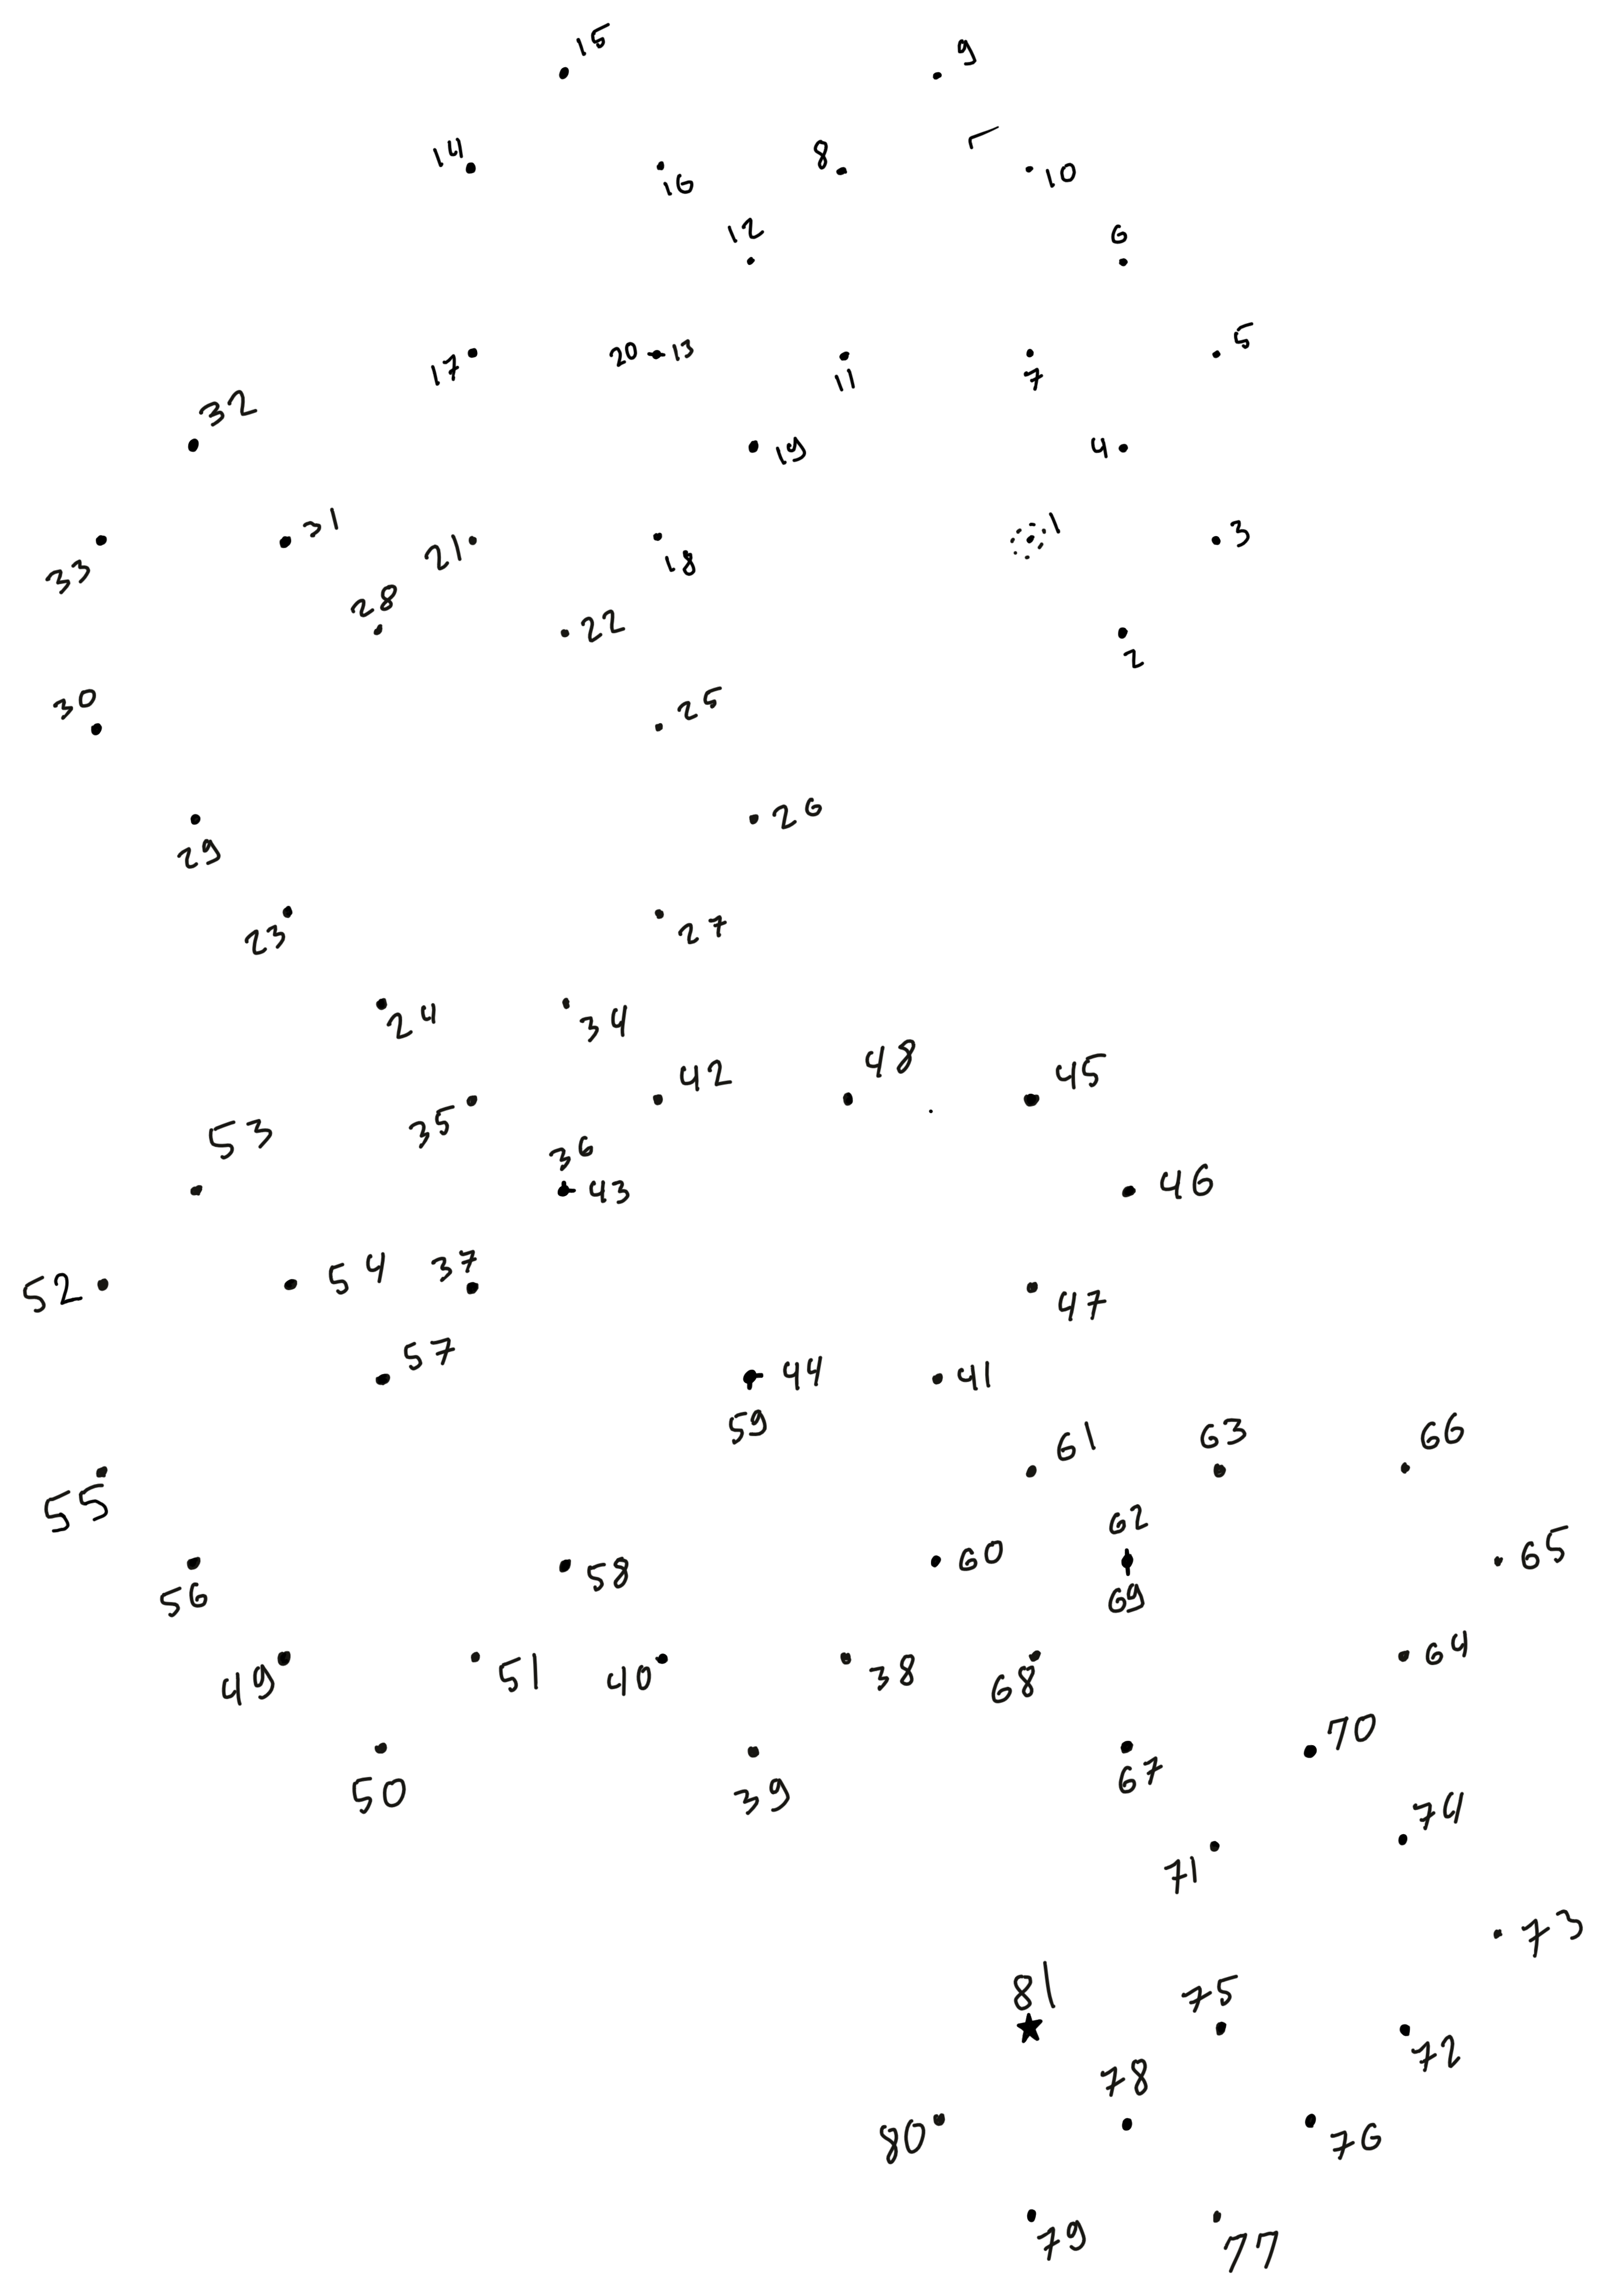
\includegraphics{A1AB5AFB-31BB-4E50-ABBE-7EDE8D4CA146.png}

This is a simple \emph{connect the dots} game. If you have this text
printed out and have a pencil handy, I encourage you to try it out and
discover the picture that hides behind those dots.

The point of this exercise is to show what happens to a linear variable
once it's consumed: It cannot be reused anymore. The dot pattern is
still visible, the numbers can still instruct you how to connect them.
But since the drawing has already been carried out, there is no possible
way to repeat the experience of connecting the dots.

Linear variables are the same, once they are used, they are ``spent''.
This is shown explicitly in Idris2's type system by using holes:

\begin{Shaded}
\begin{Highlighting}[]
\KeywordTok{let} \DecValTok{1}\NormalTok{ dots }\OtherTok{=} \DataTypeTok{MkDots}
    \DecValTok{1}\NormalTok{ drawing }\OtherTok{=}\NormalTok{ connect dots }\KeywordTok{in}
    \OperatorTok{?}\NormalTok{rest}
\end{Highlighting}
\end{Shaded}

Inspecting the hole we get:

\begin{Shaded}
\begin{Highlighting}[]
\OperatorTok{\textgreater{}}  \DecValTok{0}\NormalTok{ dots }\OperatorTok{:} \DataTypeTok{Graph}
\OperatorTok{\textgreater{}}  \DecValTok{1}\NormalTok{ drawing }\OperatorTok{:} \DataTypeTok{Graph}
\OperatorTok{\textgreater{}} \CommentTok{{-}{-}{-}{-}{-}{-}{-}{-}{-}{-}{-}{-}{-}{-}{-}{-}{-}{-}{-}{-}{-}{-}{-}{-}{-}{-}{-}{-}{-}{-}}
\OperatorTok{\textgreater{}}\NormalTok{ rest }\OperatorTok{:} \DataTypeTok{Fun}
\end{Highlighting}
\end{Shaded}

Which indicates that, while we can still \emph{see} the dots, we cannot
do anything with them, they have linearity \texttt{0}. However, we ended
up with a \texttt{drawing} that we can now use!\footnote{You will notice
  that the program asks us to return a value of type \texttt{Fun} this
  is because the goal of this exercise is to have fun.}

\hypertarget{safe-inlining-with-1}{%
\subsubsection{Safe inlining with 1}\label{safe-inlining-with-1}}

Linear variables have to be used exactly once, no less, no more. An
extremely nice property this gives us can be summarised with the
following statement:

\begin{quote}
A linear variable can always be safely inlined
\end{quote}

\emph{Inlining} refers to the ability of a compiler to replace a
function call by the body of the function. This is a typical
optimisation technique aimed at enabling further optimisations on the
resulting program.

\emph{Safely inlined} means that the inlining process will not result in
a bigger and less efficient program. Take the following example:

\begin{Shaded}
\begin{Highlighting}[]
\KeywordTok{let}\NormalTok{ x }\OtherTok{=}\NormalTok{ f y }\KeywordTok{in}
\NormalTok{    (x, x)}
\end{Highlighting}
\end{Shaded}

After inlining \texttt{x}, that is, replace every occurrence of
\texttt{x} by its definition, we obtain:

\begin{Shaded}
\begin{Highlighting}[]
\NormalTok{(f y, f y)}
\end{Highlighting}
\end{Shaded}

Which is less efficient than the original program. Indeed, imagine that
\texttt{f} is a function that takes 5 days to run. The first case calls
\texttt{f} once and duplicates its result, which would take 5 days. But
the second case calls \texttt{f} twice, which would take 10 days in
total.

If \texttt{x} were to be \emph{linear} this problem would be caught:

\begin{Shaded}
\begin{Highlighting}[]
\KeywordTok{let} \DecValTok{1}\NormalTok{ x }\OtherTok{=}\NormalTok{ f y }\KeywordTok{in}
\NormalTok{    (x, x)}
\end{Highlighting}
\end{Shaded}

\begin{Shaded}
\begin{Highlighting}[]
\OperatorTok{\textgreater{}} \DataTypeTok{There}\NormalTok{ are }\DecValTok{2}\NormalTok{ uses }\KeywordTok{of}\NormalTok{ linear variable x}
\end{Highlighting}
\end{Shaded}

Conversely, if a program typechecks while using linear variable, then
all linear variables can be inlined without loss of performance. What's
more, inlining can provide further opportunities for optimisations down
the line. In the following example, while \texttt{y} cannot be inlined,
\texttt{x} can be.

\begin{Shaded}
\begin{Highlighting}[]
\KeywordTok{let} \DecValTok{1}\NormalTok{ x }\OtherTok{=} \DecValTok{1} \OperatorTok{+} \DecValTok{3} \KeywordTok{in}
\NormalTok{    y }\OtherTok{=}\NormalTok{ x }\OperatorTok{+} \DecValTok{10} \KeywordTok{in}
\NormalTok{    (y, y)}
\end{Highlighting}
\end{Shaded}

The result of inlining \texttt{x} would be as follows\footnote{This
  example does not quite work in Idris2 as it stands, Idris2 is very
  conservative about propagating linearity to variables that are bound
  to linear function calls.}:

\begin{Shaded}
\begin{Highlighting}[]
\KeywordTok{let}\NormalTok{ y }\OtherTok{=} \DecValTok{1} \OperatorTok{+} \DecValTok{3} \OperatorTok{+} \DecValTok{10} \KeywordTok{in}
\NormalTok{    (y, y)}
\end{Highlighting}
\end{Shaded}

\hypertarget{erased-runtime-for-0}{%
\subsubsection{\texorpdfstring{Erased runtime for
\texttt{0}}{Erased runtime for 0}}\label{erased-runtime-for-0}}

In Idris2, variables can also be annotated with linearity \texttt{0},
this means that the value is \emph{inaccessible} and cannot be used. But
if that were truly the case, what would be the use of such a variable?

Those variables are particularly useful in a dependently-typed
programming language because, while they cannot be used in the body of
our program, they can be used in type signatures. Take this example with
vector:

\begin{Shaded}
\begin{Highlighting}[]
\FunctionTok{length} \OperatorTok{:} \DataTypeTok{Vect}\NormalTok{ n a }\OtherTok{{-}\textgreater{}} \DataTypeTok{Nat}
\FunctionTok{length}\NormalTok{ [] }\OtherTok{=} \DataTypeTok{Z}
\FunctionTok{length}\NormalTok{ (}\OtherTok{\_ ::}\NormalTok{ xs) }\OtherTok{=} \DataTypeTok{S}\NormalTok{ (}\FunctionTok{length}\NormalTok{ xs)}
\end{Highlighting}
\end{Shaded}

The length of the vector is computed by pattern matching on the vector
and recursively counting the length of the tail of the vector and adding
\texttt{+1} to it (recall the \texttt{S} constructor for \texttt{Nat}).
If the vector is empty, the length returned is zero (\texttt{Z}).

Another way to implement the same function in Idris1 (without linear
types) was to do the following:

\begin{Shaded}
\begin{Highlighting}[]
\CommentTok{{-}{-} This works in Idris1}
\FunctionTok{length} \OperatorTok{:} \DataTypeTok{Vect}\NormalTok{ n a }\OtherTok{{-}\textgreater{}} \DataTypeTok{Nat}
\FunctionTok{length}\NormalTok{ \_ \{n\} }\OtherTok{=}\NormalTok{ n}
\end{Highlighting}
\end{Shaded}

The \texttt{\{n\}} syntax would bring the value from the \emph{type
level} to the \emph{term level}, effectively making the type of the
vector a value that can be used within the program. However doing the
same in Idris2 is forbidden:

\begin{Shaded}
\begin{Highlighting}[]
\OperatorTok{\textgreater{}} \DataTypeTok{Error}\OperatorTok{:} \DataTypeTok{While}\NormalTok{ processing right hand side }\KeywordTok{of} \FunctionTok{length}\OperatorTok{.} 
\OperatorTok{\textgreater{}}\NormalTok{   n is }\FunctionTok{not}\NormalTok{ accessible }\KeywordTok{in}\NormalTok{ this context}\OperatorTok{.}
\OperatorTok{\textgreater{}} 
\OperatorTok{\textgreater{}}     \OperatorTok{|}
\OperatorTok{\textgreater{}}     \OperatorTok{|} \FunctionTok{length}\NormalTok{ \_ \{n\} }\OtherTok{=}\NormalTok{ n}
\OperatorTok{\textgreater{}}     \OperatorTok{|}                \OperatorTok{\^{}}
\end{Highlighting}
\end{Shaded}

It is hard to understand why this is the case just by looking at the
type signature \texttt{Vect\ n\ a\ -\textgreater{}\ Nat} and this is
because it is not complete. Behind the scenes, the Idris2 compiler is
adding implicit arguments \footnote{Implicit arguments are arguments to
  function that are not given by the programmer, but rather are filled
  in by the compiler automatically. Implicit arguments are extremely
  important in dependently-types languages because without them every
  type signature would be extremely heavy. Moreover, since the
  distinction between types and terms is blurry, the mechanism to infer
  \emph{types} is the same as the mechanism to infer \emph{terms} which
  is how the compiler can infer which value to insert whenever a
  function require an implicit argument.} for \texttt{n} and \texttt{a}
and automatically gives them linearity \texttt{0}. The full signature
looks like this:

\begin{Shaded}
\begin{Highlighting}[]
\FunctionTok{length} \OperatorTok{:}\NormalTok{ \{}\DecValTok{0}\NormalTok{ n }\OperatorTok{:} \DataTypeTok{Nat}\NormalTok{\} }\OtherTok{{-}\textgreater{}}\NormalTok{ \{}\DecValTok{0}\NormalTok{ a }\OperatorTok{:} \DataTypeTok{Type}\NormalTok{\} }\OtherTok{{-}\textgreater{}} \DataTypeTok{Vect}\NormalTok{ n a }\OtherTok{{-}\textgreater{}} \DataTypeTok{Nat}
\FunctionTok{length}\NormalTok{ \_ \{n\} }\OtherTok{=}\NormalTok{ n}
\end{Highlighting}
\end{Shaded}

The \texttt{0} means we cannot use the variable outside of the type
signature, but how come we can use them in the type signature and not to
implement our \texttt{length} function?

The difference is that linearity \texttt{0} variables are available
\emph{at compile time} and are forbidden to appear \emph{at runtime}.
The compiler can use them, compute types with them, but they cannot be
allocated and used during execution of the program we generate.

This is why linearity \texttt{0} variables are also called
\texttt{erased} variables because they are removed from the execution of
the program. We can use them to convince the compiler that some
invariants hold, but we cannot allocate any memory for them during the
execution of our program.

Finally, another subtlety is that erased variable can actually appear
inside the body of function, but only in position where they are allowed
are arguments to functions with \texttt{0} usage. Such functions are:

\hypertarget{arguments-annotated-with-0}{%
\paragraph{\texorpdfstring{1. Arguments annotated with
\texttt{0}}{1. Arguments annotated with 0}}\label{arguments-annotated-with-0}}

\begin{Shaded}
\begin{Highlighting}[]
\NormalTok{toNat }\OperatorTok{:}\NormalTok{ (}\DecValTok{0}\NormalTok{ n }\OperatorTok{:} \DataTypeTok{Nat}\NormalTok{) }\OtherTok{{-}\textgreater{}} \DataTypeTok{INat}\NormalTok{ n }\OtherTok{{-}\textgreater{}} \DataTypeTok{Nat}
\NormalTok{toNat }\DataTypeTok{Z} \DataTypeTok{Zero} \OtherTok{=} \DataTypeTok{Z}
\NormalTok{toNat (}\DataTypeTok{S}\NormalTok{ n) (}\DataTypeTok{Succ}\NormalTok{ m) }\OtherTok{=} \DataTypeTok{S}\NormalTok{ (toNat n m)}
\CommentTok{{-}{-}       ▲                      ▲}
\CommentTok{{-}{-}       │                      └ Used even if erased}
\CommentTok{{-}{-}       │}
\CommentTok{{-}{-}       └ Bound with linearity 0}
\end{Highlighting}
\end{Shaded}

Here the recursive call uses \texttt{n} which has linearity \texttt{0},
but this is allowed because the first argument of \texttt{toNat} takes
an argument of linearity \texttt{0}. In other words, \texttt{n} cannot
be consumed, but \texttt{toNat} does not consume its first argument
anyways, so all is good.

\hypertarget{rewrites}{%
\paragraph{2. Rewrites}\label{rewrites}}

\begin{Shaded}
\begin{Highlighting}[]
\NormalTok{sym }\OperatorTok{:}\NormalTok{ (}\DecValTok{0}\NormalTok{ prf }\OperatorTok{:}\NormalTok{ x }\OtherTok{=}\NormalTok{ y) }\OtherTok{{-}\textgreater{}}\NormalTok{ y }\OtherTok{=}\NormalTok{ x}
\NormalTok{sym prf }\OtherTok{=}\NormalTok{ rewrite prf }\KeywordTok{in} \DataTypeTok{Refl}
\end{Highlighting}
\end{Shaded}

Rewriting a type does not consume the proof.

\hypertarget{type-signatures}{%
\paragraph{3. Type signatures}\label{type-signatures}}

\begin{Shaded}
\begin{Highlighting}[]
\CommentTok{{-}{-}          ┌ \textasciigrave{}n\textasciigrave{} is erased}
\CommentTok{{-}{-}          ▼}
\NormalTok{reverse\textquotesingle{} }\OperatorTok{:}\NormalTok{ \{}\DecValTok{0}\NormalTok{ n }\OperatorTok{:} \DataTypeTok{Nat}\NormalTok{\} }\OtherTok{{-}\textgreater{}}\NormalTok{ (}\DecValTok{1}\NormalTok{ vs }\OperatorTok{:} \DataTypeTok{Vect}\NormalTok{ n }\DataTypeTok{Nat}\NormalTok{) }\OtherTok{{-}\textgreater{}} \DataTypeTok{Vect}\NormalTok{ n }\DataTypeTok{Nat}
\NormalTok{reverse\textquotesingle{} vs }\OtherTok{=} \KeywordTok{let}\NormalTok{ v2 }\OperatorTok{:} \DataTypeTok{Vect}\NormalTok{ n }\DataTypeTok{Nat} \OtherTok{=} \FunctionTok{reverse}\NormalTok{ vs }\KeywordTok{in}\NormalTok{ v2}
\CommentTok{{-}{-}                          ▲}
\CommentTok{{-}{-}                          └ \textasciigrave{}n\textasciigrave{} appears here}
\end{Highlighting}
\end{Shaded}

Even if \texttt{n} appears in the body of the function, appearing in a
type signature does not count as a use.

\hypertarget{no-branching-with-0}{%
\subsubsection{No branching with 0}\label{no-branching-with-0}}

In general, we cannot match on erased variables, there is however an
exception to this rule. Whenever matching on a variable \emph{does not}
result in additional branching, then we are allowed to match on this
variable, even if it erased. Such matches are called
\emph{uninformative}, and they are characterised by the fact that they
do not generate new codepaths.

No new codepaths means that, whether we match or not, the output
bytecode would be the same. The difference lies in that matching on
those variable would inform us and the compiler of very important
properties from our types. Just like the \texttt{intOrString} example
informed us of the return type of our function, an uninformative match
can reveal useful information to both the programmer and the compiler.

A good example of an uninformative match is \texttt{Refl} which has only
one constructor:

\begin{Shaded}
\begin{Highlighting}[]
\KeywordTok{data}\NormalTok{ (}\OtherTok{=}\NormalTok{) }\OperatorTok{:}\NormalTok{ (a, b }\OperatorTok{:} \DataTypeTok{Type}\NormalTok{) }\OtherTok{{-}\textgreater{}} \DataTypeTok{Type} \KeywordTok{where}
  \DataTypeTok{Refl} \OperatorTok{:}\NormalTok{ (a }\OperatorTok{:} \DataTypeTok{Type}\NormalTok{) }\OtherTok{{-}\textgreater{}}\NormalTok{ a }\OtherTok{=}\NormalTok{ a}
\end{Highlighting}
\end{Shaded}

This suggests that, even if our equality proof has linearity \texttt{0},
we can match on it, since there is only 1 constructor we are never going
to generate new branches.

But an uninformative match can also happen on types with multiple
constructors. Take this indexed \texttt{Nat} type:

\begin{Shaded}
\begin{Highlighting}[]
\KeywordTok{data} \DataTypeTok{INat} \OperatorTok{:} \DataTypeTok{Nat} \OtherTok{{-}\textgreater{}} \DataTypeTok{Type} \KeywordTok{where}
  \DataTypeTok{IZ} \OperatorTok{:} \DataTypeTok{INat} \DataTypeTok{Z}
  \DataTypeTok{IS} \OperatorTok{:} \DataTypeTok{INat}\NormalTok{ n }\OtherTok{{-}\textgreater{}} \DataTypeTok{INat}\NormalTok{ (}\DataTypeTok{S}\NormalTok{ n)}
\end{Highlighting}
\end{Shaded}

This is simply a duplicate for \texttt{Nat} but carries its own value as
index. Now let us write a function to recover the original \texttt{Nat}
from an \texttt{INat}:

\begin{Shaded}
\begin{Highlighting}[]
\NormalTok{toNat }\OperatorTok{:}\NormalTok{ (}\DecValTok{0}\NormalTok{ n }\OperatorTok{:} \DataTypeTok{Nat}\NormalTok{) }\OtherTok{{-}\textgreater{}}\NormalTok{ (}\DecValTok{1}\NormalTok{ m }\OperatorTok{:} \DataTypeTok{INat}\NormalTok{ n) }\OtherTok{{-}\textgreater{}} \DataTypeTok{Nat}
\NormalTok{toNat }\DataTypeTok{Z} \DataTypeTok{IZ} \OtherTok{=} \DataTypeTok{Z}
\NormalTok{toNat (}\DataTypeTok{S}\NormalTok{ n) (}\DataTypeTok{IS}\NormalTok{ m) }\OtherTok{=} \DataTypeTok{S}\NormalTok{ (toNat n m)}
\end{Highlighting}
\end{Shaded}

Even if we annotated \texttt{n} with linearity \texttt{0} we are allowed
to match on it. To understand why, let us add some holes and remove the
matching:

\begin{Shaded}
\begin{Highlighting}[]
\NormalTok{toNat }\OperatorTok{:}\NormalTok{ (}\DecValTok{0}\NormalTok{ n }\OperatorTok{:} \DataTypeTok{Nat}\NormalTok{) }\OtherTok{{-}\textgreater{}}\NormalTok{ (}\DecValTok{1}\NormalTok{ m }\OperatorTok{:} \DataTypeTok{INat}\NormalTok{ n) }\OtherTok{{-}\textgreater{}} \DataTypeTok{Nat}
\NormalTok{toNat n }\DataTypeTok{IZ} \OtherTok{=} \OperatorTok{?}\NormalTok{branch}
\NormalTok{toNat (}\DataTypeTok{S}\NormalTok{ n) (}\DataTypeTok{IS}\NormalTok{ m) }\OtherTok{=} \DataTypeTok{S}\NormalTok{ (toNat n m)}
\end{Highlighting}
\end{Shaded}

Idris2 will not allow this program to compile and will fail with the
following error:

\begin{Shaded}
\begin{Highlighting}[]
\OperatorTok{\textgreater{}} \DataTypeTok{Error}\OperatorTok{:} \DataTypeTok{While}\NormalTok{ processing left hand side }\KeywordTok{of}\NormalTok{ toNat}\OperatorTok{.} 
\OperatorTok{\textgreater{}}   \DataTypeTok{When}\NormalTok{ unifying }\DataTypeTok{INat} \DecValTok{0} \FunctionTok{and} \DataTypeTok{INat} \OperatorTok{?}\NormalTok{n}\OperatorTok{.}
\OperatorTok{\textgreater{}} \DataTypeTok{Pattern}\NormalTok{ variable n unifies with}\OperatorTok{:} \DecValTok{0}\OperatorTok{.}
\OperatorTok{\textgreater{}} 
\OperatorTok{\textgreater{}}     \OperatorTok{|}
\OperatorTok{\textgreater{}}     \OperatorTok{|}   \DataTypeTok{IZ} \OperatorTok{:} \DataTypeTok{INat} \DataTypeTok{Z}
\OperatorTok{\textgreater{}}     \OperatorTok{|}             \OperatorTok{\^{}}
\OperatorTok{\textgreater{}}     \OperatorTok{|}   \DataTypeTok{IS} \OperatorTok{:} \DataTypeTok{INat}\NormalTok{ n }\OtherTok{{-}\textgreater{}} \DataTypeTok{INat}\NormalTok{ (}\DataTypeTok{S}\NormalTok{ n)}
\OperatorTok{\textgreater{}}     \OperatorTok{|}\NormalTok{  toNat n }\DataTypeTok{IZ} \OtherTok{=} \OperatorTok{?}\NormalTok{branch}
\OperatorTok{\textgreater{}}     \OperatorTok{|}        \OperatorTok{\^{}}
\OperatorTok{\textgreater{}} 
\OperatorTok{\textgreater{}} \DataTypeTok{Suggestion}\OperatorTok{:} \DataTypeTok{Use}\NormalTok{ the same name for both }\KeywordTok{pattern}\NormalTok{ variables, since they }
\OperatorTok{\textgreater{}}\NormalTok{   unify}\OperatorTok{.}
\end{Highlighting}
\end{Shaded}

It tells us that \texttt{n} unifies with \texttt{Z} and forces the user
to spell out the match. Effectively forcing uninformative matches to be
made. A similar error appears if we try the same thing on the second
branch, trying to remove \texttt{S\ n}.

\newpage

\hypertarget{quantitative-type-theory-in-practice}{%
\section{Quantitative Type Theory in
practice}\label{quantitative-type-theory-in-practice}}

QTT is still a recent development and because of its young age, it has
not seen wide spread use in commercial applications. The Idris2 compiler
itself stands as the most popular example of a complex program that
showcases uses for QTT and quantitative types. Linear types already
benefit from a body of work that showcase their uses
\cite{linear_diff}\cite{linear_types_update}\cite{linear_types_session}\cite{linear_types_subst}\cite{actor_channels}\cite{linear_race}\cite{linear_use}\cite{once_upon_a_type}\cite{deforestation},
but one of the goals of this thesis was to list and discover some new
and innovative uses for linear types and QTT. In this chapter I will
mention some specific uses for QTT that I discovered during my study.

\hypertarget{limitations-and-solutions-for-quantitative-types}{%
\subsection{limitations and solutions for quantitative
types}\label{limitations-and-solutions-for-quantitative-types}}

We've seen how we can write addition of natural numbers using linear
types. But can we write a multiplication algorithm using linear types?
Let us inspect the traditional multiplication algorithm and see if we
can update it with linear types.

\hypertarget{linear-multiplication}{%
\subsubsection{Linear multiplication}\label{linear-multiplication}}

Here is a multiplication function without any linear variables

\begin{Shaded}
\begin{Highlighting}[]
\NormalTok{multiplication }\OperatorTok{:}\NormalTok{ (n }\OperatorTok{:} \DataTypeTok{Nat}\NormalTok{) }\OtherTok{{-}\textgreater{}}\NormalTok{ (m }\OperatorTok{:} \DataTypeTok{Nat}\NormalTok{) }\OtherTok{{-}\textgreater{}} \DataTypeTok{Nat}
\NormalTok{multiplication }\DataTypeTok{Z}\NormalTok{ m }\OtherTok{=} \DataTypeTok{Z} 
\NormalTok{multiplication (}\DataTypeTok{S}\NormalTok{ n) m }\OtherTok{=}\NormalTok{ m }\OperatorTok{+}\NormalTok{ (multiplication n m)}
\end{Highlighting}
\end{Shaded}

Just like with addition, we notice that some variables are only used
once, but some aren't. \texttt{n} is used exactly once in both branches,
but \texttt{m} is not used in one branch, and used twice in the other.
Which leads to the following program:

\begin{Shaded}
\begin{Highlighting}[]
\NormalTok{ multiplication }\OperatorTok{:}\NormalTok{ (}\DecValTok{1}\NormalTok{ n }\OperatorTok{:} \DataTypeTok{Nat}\NormalTok{) }\OtherTok{{-}\textgreater{}}\NormalTok{ (m }\OperatorTok{:} \DataTypeTok{Nat}\NormalTok{) }\OtherTok{{-}\textgreater{}} \DataTypeTok{Nat}
\NormalTok{ multiplication }\DataTypeTok{Z}\NormalTok{ m }\OtherTok{=} \DataTypeTok{Z}
\NormalTok{ multiplication (}\DataTypeTok{S}\NormalTok{ n) m }\OtherTok{=}\NormalTok{ m }\OperatorTok{+}\NormalTok{ (multiplication n m)}
\end{Highlighting}
\end{Shaded}

Which compiles correctly, but how could we go about implementing a
completely linear version of \texttt{mutliplication}?

indeed, writing
\texttt{multiplication\ :\ (1\ n\ :\ Nat)\ -\textgreater{}\ (0\ m\ :\ Nat)\ -\textgreater{}\ Nat}
gets us the error:

\begin{Shaded}
\begin{Highlighting}[]
\DataTypeTok{Error}\OperatorTok{:} \DataTypeTok{While}\NormalTok{ processing right hand side }\KeywordTok{of}\NormalTok{ multiplication}\OperatorTok{.} 
\NormalTok{    m is }\FunctionTok{not}\NormalTok{ accessible }\KeywordTok{in}\NormalTok{ this context}\OperatorTok{.}

    \OperatorTok{|}
    \OperatorTok{|}\NormalTok{ multiplication (}\DataTypeTok{S}\NormalTok{ n) m }\OtherTok{=}\NormalTok{ m }\OperatorTok{+}\NormalTok{ (multiplication n m)}
    \OperatorTok{|}                          \OperatorTok{\^{}}
\end{Highlighting}
\end{Shaded}

Which catches the fact that \texttt{m} is use twice in the second branch
(but the first branch is fine).

Ideally we would like to write this program:

\begin{Shaded}
\begin{Highlighting}[]
\CommentTok{{-}{-}        The multiplicity depends on the first arugment}
\CommentTok{{-}{-}                               ▼}
\NormalTok{multiplication }\OperatorTok{:}\NormalTok{ (}\DecValTok{1}\NormalTok{ n }\OperatorTok{:} \DataTypeTok{Nat}\NormalTok{) }\OtherTok{{-}\textgreater{}}\NormalTok{ (n m }\OperatorTok{:} \DataTypeTok{Nat}\NormalTok{) }\OtherTok{{-}\textgreater{}} \DataTypeTok{Nat}
\NormalTok{multiplication }\DataTypeTok{Z}\NormalTok{ m }\OtherTok{=} \DataTypeTok{Z}
\NormalTok{multiplication (}\DataTypeTok{S}\NormalTok{ n) m }\OtherTok{=}\NormalTok{ m }\OperatorTok{+}\NormalTok{ (multiplication n m)}
\end{Highlighting}
\end{Shaded}

However Idris2 and QTT do not support \emph{dependent linearities} or
\emph{first class linearity} where linearity annotations are values
within the language.

We can however attempt to replicate this behaviour with different
proxies:

\begin{Shaded}
\begin{Highlighting}[]
\NormalTok{provide }\OperatorTok{:} \DataTypeTok{Copy}\NormalTok{ t }\OtherTok{=\textgreater{}} \DataTypeTok{Drop}\NormalTok{ t }\OtherTok{=\textgreater{}}\NormalTok{ (}\DecValTok{1}\NormalTok{ n }\OperatorTok{:} \DataTypeTok{Nat}\NormalTok{) }\OtherTok{{-}\textgreater{}}\NormalTok{ (}\DecValTok{1}\NormalTok{ v }\OperatorTok{:}\NormalTok{ t) }
       \OtherTok{{-}\textgreater{}}\NormalTok{ (}\DataTypeTok{DPair} \DataTypeTok{Nat}\NormalTok{ (\textbackslash{}x }\OtherTok{=\textgreater{}}\NormalTok{ n }\OtherTok{=}\NormalTok{ x), }\DataTypeTok{Vect}\NormalTok{ n t)}
\NormalTok{provide }\DecValTok{0}\NormalTok{ v }\OtherTok{=} \KeywordTok{let}\NormalTok{ () }\OtherTok{=} \FunctionTok{drop}\NormalTok{ v }\KeywordTok{in}\NormalTok{ (}\DataTypeTok{MkDPair} \DataTypeTok{Z} \DataTypeTok{Refl}\NormalTok{, [])}
\NormalTok{provide (}\DataTypeTok{S}\NormalTok{ k) v }\OtherTok{=} \KeywordTok{let}\NormalTok{ (v1, v2) }\OtherTok{=}\NormalTok{ copy v}
\NormalTok{                      (}\DataTypeTok{MkDPair}\NormalTok{ n prf, vs) }\OtherTok{=}\NormalTok{ provide k v1}
                   \KeywordTok{in} \DataTypeTok{MkDPair}\NormalTok{ (}\DataTypeTok{S}\NormalTok{ n) (cong }\DataTypeTok{S}\NormalTok{ prf),}\OtherTok{ v2 ::}\NormalTok{ vs)}

\NormalTok{multiplication }\OperatorTok{:}\NormalTok{ (}\DecValTok{1}\NormalTok{ n, m }\OperatorTok{:} \DataTypeTok{Nat}\NormalTok{) }\OtherTok{{-}\textgreater{}} \DataTypeTok{Nat}
\NormalTok{multiplication n m }\OtherTok{=} \KeywordTok{let}\NormalTok{ (}\DataTypeTok{MkDPair}\NormalTok{ n\textquotesingle{} }\DataTypeTok{Refl}\NormalTok{, ms) }\OtherTok{=}\NormalTok{ provide n m }\KeywordTok{in}\NormalTok{ mult n\textquotesingle{} ms}
  \KeywordTok{where}
\NormalTok{    mult }\OperatorTok{:}\NormalTok{ (}\DecValTok{1}\NormalTok{ n }\OperatorTok{:} \DataTypeTok{Nat}\NormalTok{) }\OtherTok{{-}\textgreater{}}\NormalTok{ (}\DecValTok{1}\NormalTok{ vs }\OperatorTok{:} \DataTypeTok{Vect}\NormalTok{ n }\DataTypeTok{Nat}\NormalTok{) }\OtherTok{{-}\textgreater{}} \DataTypeTok{Nat}
\NormalTok{    mult }\DecValTok{0}\NormalTok{ [] }\OtherTok{=} \DecValTok{0}
\NormalTok{    mult (}\DataTypeTok{S}\NormalTok{ k) (}\OtherTok{m ::}\NormalTok{ x) }\OtherTok{=}\NormalTok{ m }\OperatorTok{+}\NormalTok{ (mult k x)}
\end{Highlighting}
\end{Shaded}

This program attempts to simulate the previous signature by creating a
dependency between \texttt{n} and a vector of length \texttt{n}
containing copies of the variable \texttt{m}\footnote{For the purposes
  of this example there is no proof that the vector \emph{actually}
  contains only copies of \texttt{m} but this is an invariant that could
  be implemented at the type level. But doing so would introduce lots of
  equality proofs which would render the code even harder to read.} with
the type
\texttt{mult\ :\ (1\ n\ :\ Nat)\ -\textgreater{}\ (1\ \_\ :\ Vect\ n\ Nat)\ -\textgreater{}\ Nat~}.

As we've demonstrated, we technically can express more complex
relationship between linear types provided they implement our interfaces
\texttt{Drop} and \texttt{Copy}. However, the extra work to make the
dependency explicit in the type isn't worth the effort. Indeed, giving
up this dependency allows us to write the following program:

\begin{Shaded}
\begin{Highlighting}[]
\NormalTok{lmult }\OperatorTok{:}\NormalTok{ (}\DecValTok{1}\NormalTok{ n, m }\OperatorTok{:} \DataTypeTok{Nat}\NormalTok{) }\OtherTok{{-}\textgreater{}} \DataTypeTok{Nat}
\NormalTok{lmult }\DecValTok{0}\NormalTok{ m }\OtherTok{=} \KeywordTok{let}\NormalTok{ () }\OtherTok{=} \FunctionTok{drop}\NormalTok{ m }\KeywordTok{in} \DataTypeTok{Z}
\NormalTok{lmult (}\DataTypeTok{S}\NormalTok{ k) m }\OtherTok{=} \KeywordTok{let}\NormalTok{ (a, b) }\OtherTok{=}\NormalTok{ copy m }\KeywordTok{in}\NormalTok{ a }\OperatorTok{+}\NormalTok{ lmult k b}
\end{Highlighting}
\end{Shaded}

Which is a lot simpler and achieves the same goal, it even has the same
performance characteristics.

\hypertarget{permutations}{%
\subsection{Permutations}\label{permutations}}

The following example is certainly my favourite since it combines both
dependent types and linear types in a way that wasn't possible before.
It has been done in the context of my work for Statebox, a company that
strongly relies on dependent types to write formally verified software.

One of their project is a validator for petri-nets\cite{petri-nets} and
petri-net executions:
\href{https://github.com/statebox/fsm-oracle}{FSM-oracle}\footnote{\url{https://github.com/statebox/fsm-oracle}}.
While the technical details of this projects are outside the scope of
this text, there is one aspect of it that is fundamentally linked with
linear types, and that is the concept of permutation.

FSM-Oracle describes petri-nets using
\href{http://www.zanasi.com/fabio/files/paperCALCO19b.pdf}{\emph{hypergraphs}}
\cite{cartographer} those hypergraphs use
\href{https://github.com/statebox/fsm-oracle/blob/master/src/Permutations/Permutations.idr\#L31}{\emph{permutations}~}\footnote{\url{https://github.com/statebox/fsm-oracle/blob/master/src/Permutations/Permutations.idr\#L31}}
in order to model that wire inside it can be moved around. This concept
is key in a correct and proven implementation of hypergraphs. However,
permutations turn out to be extremely complex to implement using only
dependent types as can attest the files
\href{https://github.com/statebox/fsm-oracle/blob/master/src/Permutations/PermutationsCategory.idr}{trying
to fit}\footnote{\url{https://github.com/statebox/fsm-oracle/blob/master/src/Permutations/PermutationsCategory.idr}}
their definition into a
\href{https://github.com/statebox/fsm-oracle/blob/master/src/Permutations/PermutationsStrictMonoidalCategory.idr}{Category}\footnote{\url{https://github.com/statebox/fsm-oracle/blob/master/src/Permutations/PermutationsStrictMonoidalCategory.idr}}.

The relevant bit about permutation can be found in the two files
\texttt{Permutations.idr} and \texttt{SwapDown.idr}, a permutation
relies on a list of ``swaps'' that describe the operation that we can do
on a list to generate a new permutation of the same list.

\begin{Shaded}
\begin{Highlighting}[]
\KeywordTok{data} \DataTypeTok{Perm} \OperatorTok{:}\NormalTok{ \{o }\OperatorTok{:} \DataTypeTok{Type}\NormalTok{\} }\OtherTok{{-}\textgreater{}} \DataTypeTok{List}\NormalTok{ o }\OtherTok{{-}\textgreater{}} \DataTypeTok{List}\NormalTok{ o }\OtherTok{{-}\textgreater{}} \DataTypeTok{Type} \KeywordTok{where}
  \DataTypeTok{Nil} \OperatorTok{:} \DataTypeTok{Perm}\NormalTok{ [] []}
  \DataTypeTok{Ins} \OperatorTok{:} \DataTypeTok{Perm}\NormalTok{ xs ys }\OtherTok{{-}\textgreater{}} \DataTypeTok{SwapDown}\NormalTok{ (}\OtherTok{a::}\NormalTok{ys) zs }\OtherTok{{-}\textgreater{}} \DataTypeTok{Perm}\NormalTok{ (}\OtherTok{a::}\NormalTok{xs) zs}

\KeywordTok{data} \DataTypeTok{SwapDown} \OperatorTok{:} \DataTypeTok{List}\NormalTok{ t }\OtherTok{{-}\textgreater{}} \DataTypeTok{List}\NormalTok{ t }\OtherTok{{-}\textgreater{}} \DataTypeTok{Type} \KeywordTok{where}
  \DataTypeTok{HereS}  \OperatorTok{:} \DataTypeTok{SwapDown}\NormalTok{ (}\OtherTok{a::}\NormalTok{as) (}\OtherTok{a::}\NormalTok{as)}
  \DataTypeTok{ThereS} \OperatorTok{:} \DataTypeTok{SwapDown}\NormalTok{ (}\OtherTok{a::}\NormalTok{as) bs }\OtherTok{{-}\textgreater{}} \DataTypeTok{SwapDown}\NormalTok{ (}\OtherTok{a::b::}\NormalTok{as) (}\OtherTok{b::}\NormalTok{bs)}
\end{Highlighting}
\end{Shaded}

If you don't have access to the internet to witness the proofs in their
full glory, here is an example of what we are dealing with:

\begin{Shaded}
\begin{Highlighting}[]
\NormalTok{permAssoc }\OperatorTok{:}\NormalTok{ (ab }\OperatorTok{:} \DataTypeTok{Perm}\NormalTok{ aas bbs) }\OtherTok{{-}\textgreater{}}\NormalTok{ (bc }\OperatorTok{:} \DataTypeTok{Perm}\NormalTok{ bbs ccs) }
         \OtherTok{{-}\textgreater{}}\NormalTok{ (cd }\OperatorTok{:} \DataTypeTok{Perm}\NormalTok{ ccs dds)}
         \OtherTok{{-}\textgreater{}}\NormalTok{ permComp ab (permComp bc cd) }\OtherTok{=}\NormalTok{ permComp (permComp ab bc) cd}
\NormalTok{permAssoc }\DataTypeTok{Nil}\NormalTok{ bc cd }\OtherTok{=} \DataTypeTok{Refl}
\NormalTok{permAssoc (}\DataTypeTok{Ins}\NormalTok{ \{xs}\OtherTok{=}\NormalTok{as\} \{ys}\OtherTok{=}\NormalTok{bs\} ab\textquotesingle{} abb) bc cd }
\NormalTok{  with (shuffle abb (permComp bc cd)) proof bdPrf}
  \OperatorTok{|} \DataTypeTok{Ins}\NormalTok{ \{ys}\OtherTok{=}\NormalTok{ds\} bd\textquotesingle{} add with (shuffle abb bc) proof bcPrf}
    \OperatorTok{|} \DataTypeTok{Ins}\NormalTok{ \{ys}\OtherTok{=}\NormalTok{cs\} bc\textquotesingle{} acc with (shuffle acc cd) proof cdPrf}
      \OperatorTok{|} \DataTypeTok{Ins}\NormalTok{ \{ys}\OtherTok{=}\NormalTok{ds\textquotesingle{}\} cd\textquotesingle{} ad\textquotesingle{}d }\OtherTok{=}
        \KeywordTok{let}\NormalTok{ (}\DataTypeTok{Refl}\NormalTok{, }\DataTypeTok{Refl}\NormalTok{, }\DataTypeTok{Refl}\NormalTok{) }\OtherTok{=}\NormalTok{ shuffleComp abb bc cd bcPrf cdPrf bdPrf}
         \KeywordTok{in}\NormalTok{ insCong5 }\DataTypeTok{Refl} \DataTypeTok{Refl} \DataTypeTok{Refl}\NormalTok{ (permAssoc ab\textquotesingle{} bc\textquotesingle{} cd\textquotesingle{}) }\DataTypeTok{Refl}
\end{Highlighting}
\end{Shaded}

This function ensures that composition of permutation is associative. It
relies on helper functions such as \texttt{shuffleComp} which are not
even implemented in Idris1, because it is too hard to implemnt.

Linear types can thankfully ease the pain by providing a very simple
representation of permutations :

\begin{Shaded}
\begin{Highlighting}[]
\DataTypeTok{Permutation} \OperatorTok{:} \DataTypeTok{Type} \OtherTok{{-}\textgreater{}} \DataTypeTok{Type}
\DataTypeTok{Permutation}\NormalTok{ a }\OtherTok{=}\NormalTok{ (}\DecValTok{1}\NormalTok{ ls }\OperatorTok{:} \DataTypeTok{List}\NormalTok{ a) }\OtherTok{{-}\textgreater{}} \DataTypeTok{List}\NormalTok{ a}
\end{Highlighting}
\end{Shaded}

That is, a \texttt{Permutation} parameterised over a type \texttt{a} is
a linear function from \texttt{List\ a} to \texttt{List\ a}\footnote{This
  has already been formally proven by Bob Atkey
  \url{https://github.com/bobatkey/sorting-types/blob/master/agda/Linear.agda}}.

This definition works because no elements from the input list can be
omitted or reused for the output list. \emph{Every single element} from
the argument has to find a new spot in the output list. Additionally,
since the type \texttt{a} is unknown, no special value can be inserted
in advance. Indeed, the only way to achieve this effect would be to
pattern match on \texttt{a} and create values once \texttt{a} is known,
but this would require \texttt{a} to be bound with a multiplicity
greater than \texttt{0}:

\begin{Shaded}
\begin{Highlighting}[]
\NormalTok{fakePermutation }\OperatorTok{:}\NormalTok{ \{a }\OperatorTok{:} \DataTypeTok{Type}\NormalTok{\} }\OtherTok{{-}\textgreater{}}\NormalTok{ (}\DecValTok{1}\NormalTok{ \_ }\OperatorTok{:} \DataTypeTok{List}\NormalTok{ a) }\OtherTok{{-}\textgreater{}} \DataTypeTok{List}\NormalTok{ a}
\NormalTok{fakePermutatoin \{a }\OtherTok{=} \DataTypeTok{Int}\NormalTok{\} ls }\OtherTok{=} \DecValTok{42}\OtherTok{ ::}\NormalTok{ ls}
\NormalTok{fakePermutation \{a }\OtherTok{=}\NormalTok{ \_\} ls }\OtherTok{=} \FunctionTok{reverse}\NormalTok{ ls}
\end{Highlighting}
\end{Shaded}

In this example, \texttt{a} is bound with \emph{unrestricted}
multiplicity, which give us the hint that it \emph{is} inspected and the
permutation might not be a legitimate permutation.

What's more, viewing permutations as a function gives it extremely
simple categorical semantics: It is just an instance of the category of
types with linear functions as morphisms.

Assuming \texttt{Category} is defined this way:

\begin{Shaded}
\begin{Highlighting}[]
\CommentTok{{-}{-} operator for composition}
\NormalTok{infix }\DecValTok{2} \OperatorTok{.*.}
\CommentTok{{-}{-} operator for morphisms}
\KeywordTok{infixr} \DecValTok{1} \OperatorTok{\textasciitilde{}\textgreater{}}

\NormalTok{record }\DataTypeTok{Category}\NormalTok{ (obj }\OperatorTok{:} \DataTypeTok{Type}\NormalTok{)  }\KeywordTok{where}
\NormalTok{  constructor }\DataTypeTok{MkCategory}
\NormalTok{  (}\OperatorTok{\textasciitilde{}\textgreater{}}\NormalTok{)          }\OperatorTok{:}\NormalTok{ obj }\OtherTok{{-}\textgreater{}}\NormalTok{ obj }\OtherTok{{-}\textgreater{}} \DataTypeTok{Type} \CommentTok{{-}{-} morphism}
\NormalTok{  identity      }\OperatorTok{:}\NormalTok{ \{}\DecValTok{0}\NormalTok{ a }\OperatorTok{:}\NormalTok{ obj\} }\OtherTok{{-}\textgreater{}}\NormalTok{ a }\OperatorTok{\textasciitilde{}\textgreater{}}\NormalTok{ a}
\NormalTok{  (}\OperatorTok{.*.}\NormalTok{)         }\OperatorTok{:}\NormalTok{ \{}\DecValTok{0}\NormalTok{ a, b, c}\OperatorTok{:}\NormalTok{ obj\}}
               \OtherTok{{-}\textgreater{}}\NormalTok{ (a }\OperatorTok{\textasciitilde{}\textgreater{}}\NormalTok{ b)}
               \OtherTok{{-}\textgreater{}}\NormalTok{ (b }\OperatorTok{\textasciitilde{}\textgreater{}}\NormalTok{ c)}
               \OtherTok{{-}\textgreater{}}\NormalTok{ (a }\OperatorTok{\textasciitilde{}\textgreater{}}\NormalTok{ c)}
\NormalTok{  leftIdentity  }\OperatorTok{:}\NormalTok{ \{}\DecValTok{0}\NormalTok{ a, b }\OperatorTok{:}\NormalTok{ obj\}}
               \OtherTok{{-}\textgreater{}}\NormalTok{ (f }\OperatorTok{:}\NormalTok{ a }\OperatorTok{\textasciitilde{}\textgreater{}}\NormalTok{ b)}
               \OtherTok{{-}\textgreater{}}\NormalTok{ identity }\OperatorTok{.*.}\NormalTok{ f }\OtherTok{=}\NormalTok{ f}
\NormalTok{  rightIdentity }\OperatorTok{:}\NormalTok{ \{}\DecValTok{0}\NormalTok{ a, b }\OperatorTok{:}\NormalTok{ obj\}}
               \OtherTok{{-}\textgreater{}}\NormalTok{ (f }\OperatorTok{:}\NormalTok{ a }\OperatorTok{\textasciitilde{}\textgreater{}}\NormalTok{ b)}
               \OtherTok{{-}\textgreater{}}\NormalTok{ f }\OperatorTok{.*.}\NormalTok{ identity }\OtherTok{=}\NormalTok{ f}
\NormalTok{  associativity }\OperatorTok{:}\NormalTok{ \{}\DecValTok{0}\NormalTok{ a, b, c, d }\OperatorTok{:}\NormalTok{ obj\}}
               \OtherTok{{-}\textgreater{}}\NormalTok{ (f }\OperatorTok{:}\NormalTok{ a }\OperatorTok{\textasciitilde{}\textgreater{}}\NormalTok{ b)}
               \OtherTok{{-}\textgreater{}}\NormalTok{ (g }\OperatorTok{:}\NormalTok{ b }\OperatorTok{\textasciitilde{}\textgreater{}}\NormalTok{ c)}
               \OtherTok{{-}\textgreater{}}\NormalTok{ (h }\OperatorTok{:}\NormalTok{ c }\OperatorTok{\textasciitilde{}\textgreater{}}\NormalTok{ d)}
               \OtherTok{{-}\textgreater{}}\NormalTok{ f }\OperatorTok{.*.}\NormalTok{ (g }\OperatorTok{.*.}\NormalTok{ h) }\OtherTok{=}\NormalTok{ (f }\OperatorTok{.*.}\NormalTok{ g) }\OperatorTok{.*.}\NormalTok{ h}
\end{Highlighting}
\end{Shaded}

We can write and instance of \texttt{Category} for \texttt{List\ o}:

\begin{Shaded}
\begin{Highlighting}[]
\DataTypeTok{Permutation} \OperatorTok{:} \DataTypeTok{List}\NormalTok{ o }\OtherTok{{-}\textgreater{}} \DataTypeTok{List}\NormalTok{ o }\OtherTok{{-}\textgreater{}} \DataTypeTok{Type}
\DataTypeTok{Permutation}\NormalTok{ a b }\OtherTok{=} \DataTypeTok{Same}\NormalTok{ a b}

\NormalTok{permutationCategory }\OperatorTok{:} \DataTypeTok{Category}\NormalTok{ (}\DataTypeTok{List}\NormalTok{ o)}
\NormalTok{permutationCategory }\OtherTok{=} \DataTypeTok{MkCategory}
  \DataTypeTok{Permutation}
\NormalTok{  sid}
\NormalTok{  linCompose}
\NormalTok{  linLeftIdentity}
\NormalTok{  linRightIdentity}
\NormalTok{  linAssoc}
\end{Highlighting}
\end{Shaded}

Using the definitions and lemmas for \texttt{Same} which is a data type
that represents a linear function between two values of the same type:

\begin{Shaded}
\begin{Highlighting}[]
\CommentTok{{-}{-} a linear function between two values of the same type}
\NormalTok{record }\DataTypeTok{Same}\NormalTok{ \{}\DecValTok{0}\NormalTok{ o }\OperatorTok{:} \DataTypeTok{Type}\NormalTok{\} (input, output }\OperatorTok{:}\NormalTok{ o) }\KeywordTok{where}
\NormalTok{  constructor }\DataTypeTok{MkSame}
\NormalTok{  func }\OperatorTok{:} \DataTypeTok{LinearFn}\NormalTok{ o o}
  \CommentTok{{-}{-} check the codomain of the function is correct}
\NormalTok{  check }\OperatorTok{:}\NormalTok{ (func }\OtherTok{\textasciigrave{}lapp\textasciigrave{}}\NormalTok{ input) }\OtherTok{=}\NormalTok{ output}

\NormalTok{sid }\OperatorTok{:} \DataTypeTok{Same}\NormalTok{ a a}
\NormalTok{sid }\OtherTok{=} \DataTypeTok{MkSame}\NormalTok{ lid }\DataTypeTok{Refl}

\NormalTok{linCompose }\OperatorTok{:}\NormalTok{ \{}\DecValTok{0}\NormalTok{ o }\OperatorTok{:} \DataTypeTok{Type}\NormalTok{\}}
  \OtherTok{{-}\textgreater{}}\NormalTok{ \{}\DecValTok{0}\NormalTok{ a, b, c }\OperatorTok{:}\NormalTok{ o\}}
  \OtherTok{{-}\textgreater{}} \DataTypeTok{Same}\NormalTok{ a b}
  \OtherTok{{-}\textgreater{}} \DataTypeTok{Same}\NormalTok{ b c}
  \OtherTok{{-}\textgreater{}} \DataTypeTok{Same}\NormalTok{ a c}
\NormalTok{linCompose (}\DataTypeTok{MkSame}\NormalTok{ fn }\DataTypeTok{Refl}\NormalTok{) (}\DataTypeTok{MkSame}\NormalTok{ gn }\DataTypeTok{Refl}\NormalTok{)}
  \OtherTok{=} \DataTypeTok{MkSame}\NormalTok{ (lcomp fn gn) }\DataTypeTok{Refl}

\NormalTok{linRightIdentity }\OperatorTok{:}\NormalTok{ \{}\DecValTok{0}\NormalTok{ o }\OperatorTok{:} \DataTypeTok{Type}\NormalTok{\}}
   \OtherTok{{-}\textgreater{}}\NormalTok{ \{}\DecValTok{0}\NormalTok{ a, b }\OperatorTok{:}\NormalTok{ o\}}
   \OtherTok{{-}\textgreater{}}\NormalTok{ (f }\OperatorTok{:} \DataTypeTok{Same}\NormalTok{ a b)}
   \OtherTok{{-}\textgreater{}}\NormalTok{ linCompose f (}\DataTypeTok{MkSame}\NormalTok{ Main.lid }\DataTypeTok{Refl}\NormalTok{) }\OtherTok{=}\NormalTok{ f}
\NormalTok{linRightIdentity (}\DataTypeTok{MkSame}\NormalTok{ (}\DataTypeTok{MkLin}\NormalTok{ fn) }\DataTypeTok{Refl}\NormalTok{) }\OtherTok{=} \DataTypeTok{Refl}

\NormalTok{linLeftIdentity }\OperatorTok{:}\NormalTok{ \{}\DecValTok{0}\NormalTok{ o }\OperatorTok{:} \DataTypeTok{Type}\NormalTok{\}}
   \OtherTok{{-}\textgreater{}}\NormalTok{ \{}\DecValTok{0}\NormalTok{ a, b }\OperatorTok{:}\NormalTok{ o\}}
   \OtherTok{{-}\textgreater{}}\NormalTok{ (f }\OperatorTok{:} \DataTypeTok{Same}\NormalTok{ a b)}
   \OtherTok{{-}\textgreater{}}\NormalTok{ linCompose (}\DataTypeTok{MkSame}\NormalTok{ Main.lid }\DataTypeTok{Refl}\NormalTok{) f }\OtherTok{=}\NormalTok{ f}
\NormalTok{linLeftIdentity (}\DataTypeTok{MkSame}\NormalTok{ (}\DataTypeTok{MkLin}\NormalTok{ fn) }\DataTypeTok{Refl}\NormalTok{) }\OtherTok{=} \DataTypeTok{Refl}

\NormalTok{linAssoc }\OperatorTok{:}\NormalTok{ (f }\OperatorTok{:} \DataTypeTok{Same}\NormalTok{ a b) }\OtherTok{{-}\textgreater{}}
\NormalTok{           (g }\OperatorTok{:} \DataTypeTok{Same}\NormalTok{ b c) }\OtherTok{{-}\textgreater{}}
\NormalTok{           (h }\OperatorTok{:} \DataTypeTok{Same}\NormalTok{ c d) }\OtherTok{{-}\textgreater{}}
\NormalTok{           linCompose f (linCompose g h) }\OtherTok{=}\NormalTok{ linCompose (linCompose f g) h}
\NormalTok{linAssoc (}\DataTypeTok{MkSame}\NormalTok{ (}\DataTypeTok{MkLin}\NormalTok{ fn) }\DataTypeTok{Refl}\NormalTok{)}
\NormalTok{         (}\DataTypeTok{MkSame}\NormalTok{ (}\DataTypeTok{MkLin}\NormalTok{ gn) }\DataTypeTok{Refl}\NormalTok{)}
\NormalTok{         (}\DataTypeTok{MkSame}\NormalTok{ (}\DataTypeTok{MkLin}\NormalTok{ hn) }\DataTypeTok{Refl}\NormalTok{) }\OtherTok{=} \DataTypeTok{Refl}
\end{Highlighting}
\end{Shaded}

\texttt{LinearFunction} is defined as follows:

\begin{Shaded}
\begin{Highlighting}[]
\NormalTok{record }\DataTypeTok{LinearFn}\NormalTok{ (a, b }\OperatorTok{:} \DataTypeTok{Type}\NormalTok{) }\KeywordTok{where}
\NormalTok{  constructor }\DataTypeTok{MkLin}
\NormalTok{  fn }\OperatorTok{:}\NormalTok{ (}\DecValTok{1}\NormalTok{ \_ }\OperatorTok{:}\NormalTok{ a) }\OtherTok{{-}\textgreater{}}\NormalTok{ b}

\NormalTok{lid }\OperatorTok{:} \DataTypeTok{LinearFn}\NormalTok{ a a}
\NormalTok{lid }\OtherTok{=} \DataTypeTok{MkLin}\NormalTok{ (\textbackslash{}}\DecValTok{1}\NormalTok{ x }\OtherTok{=\textgreater{}}\NormalTok{ x)}

\NormalTok{lapp }\OperatorTok{:} \DataTypeTok{LinearFn}\NormalTok{ a b }\OtherTok{{-}\textgreater{}}\NormalTok{ (}\DecValTok{1}\NormalTok{ \_ }\OperatorTok{:}\NormalTok{ a) }\OtherTok{{-}\textgreater{}}\NormalTok{ b}
\NormalTok{lapp f a }\OtherTok{=}\NormalTok{ f}\OperatorTok{.}\NormalTok{fn a}

\NormalTok{lcomp }\OperatorTok{:} \DataTypeTok{LinearFn}\NormalTok{ a b }\OtherTok{{-}\textgreater{}} \DataTypeTok{LinearFn}\NormalTok{ b c }\OtherTok{{-}\textgreater{}} \DataTypeTok{LinearFn}\NormalTok{ a c}
\NormalTok{lcomp f g }\OtherTok{=} \DataTypeTok{MkLin}\NormalTok{ (\textbackslash{}}\DecValTok{1}\NormalTok{ x }\OtherTok{=\textgreater{}}\NormalTok{ g}\OperatorTok{.}\NormalTok{fn (f}\OperatorTok{.}\NormalTok{fn x))}
\end{Highlighting}
\end{Shaded}

While this looks like a lot of code, the entire definition holds within
100 lines (including the \texttt{Category} definition), and a lot of the
definitions like \texttt{LinearFn} and \texttt{Same} are generic enough
to be reused in other modules.

Additionally, this approach is extremely straightforward. So much that
in the future, it wouldn't seem extravagant to have the type-system
automatically generate the code as part of a derived interface.

Finally and most importantly, this program could not exist without using
both dependent types to declare the necessary proofs to formally
verified our Categorical structure, and linear types to implement
\texttt{Permutation}. It is a beautiful example where the two features
meet and merge in a way that is both practical and elegant.

\hypertarget{levitation-improvements}{%
\subsection{Levitation improvements}\label{levitation-improvements}}

\emph{The gentle art of levitation}\cite{levitation} shows that a
dependently typed language has enough resources to describe all indexed
data types with only a few constructors. The ability to define types as
a language library rather than a language features allows a great deal
of introspection which in turns allows a realm of possibilities. Indeed,
we can now define operations on those data types that will preserve the
semantics of the type but make the representation more efficient. We can
generate interface implementations for them automatically. And we can
use them to construct new types out of existing
ones\cite{category_of_containers}\cite{delta_for_data}\cite{indexed_containers},
including representations for primitive types such as \texttt{Int} or
\texttt{String}, an approach that's been proven effective with
Typedefs\cite{typedefs}.

\emph{The practical guide to levitation}\cite{levitation} shows that
those features are plagued by multiple shortcomings: the verbosity of
the definitions not only make the data declaration hard to write and
read, it makes the compiler spend a lot of time constructing and
checking those terms and it has trouble identifying what is a type
parameter or what is an index.

Thankfully, the performance inefficiency from levitation can be
alleviated by a smart use of erasure. In his thesis, Ahmad Salim relies
on erasing terms with the \texttt{.} (dot) syntax, which does its best
but cannot enforce erasure of terms.

While the following has not been implemented, it shows Idris2 has a lot
of promise in lifting previous performance limitations. This is because,
in Idris2, we can perform and enforce erasure by annotating
well-formedness proofs with \texttt{0} and use data types such as
\texttt{Exists} instead of \texttt{DPair}.

More challenges arise when we try to use levitation to represent Idris
data definitions. Indeed, linear and erased variables in constructors
cannot be represented. We cannot represent the following constructor.

\begin{Shaded}
\begin{Highlighting}[]
\NormalTok{(}\OtherTok{::}\NormalTok{) }\OperatorTok{:}\NormalTok{ \{n }\OperatorTok{:} \DataTypeTok{Nat}\NormalTok{\} }\OtherTok{{-}\textgreater{}}\NormalTok{ \{}\DecValTok{0}\NormalTok{ a }\OperatorTok{:} \DataTypeTok{Type}\NormalTok{\} }\OtherTok{{-}\textgreater{}}\NormalTok{ a }\OtherTok{{-}\textgreater{}} \DataTypeTok{Vect}\NormalTok{ n a }\OtherTok{{-}\textgreater{}} \DataTypeTok{Vect}\NormalTok{ (}\DataTypeTok{S}\NormalTok{ n) a }
\end{Highlighting}
\end{Shaded}

This suggests that levitation could be extended to support constructor
with linear and erased arguments, but the it's unknown if
\emph{levitation} itself (defining the description of linear data types
in terms of itself) would be achievable.

Interestingly enough, encoding linearity in levitated description might
also help fix one of the shortcoming of levitation in idris:
automatically discerning between type parameters and type indices.
Combined with the ability to pattern match on types, in turn would allow
the Idris2 compiler to generate definitions for interfaces such as
\texttt{Functor} and \texttt{Applicative}.

\hypertarget{compile-time-string-concatenation}{%
\subsection{Compile-time string
concatenation}\label{compile-time-string-concatenation}}

Strings are ubiquitous in programming. That is why a lot of programming
languages have spent a considerable effort in optimising string usage
and string API ergonomics. Most famously, Perl is notorious for its
extensive and powerful string manipulation API including first-class
regex support with more recent additions including built-in support for
grammars.

One very popular feature to ease the ergonomics of string literals is
\emph{string interpolation}. String interpolation allows you to avoid
this situation

\begin{Shaded}
\begin{Highlighting}[]
\FunctionTok{show}\NormalTok{ (}\DataTypeTok{MyData}\NormalTok{ arg1 arg2 arg3 arg4) }\OtherTok{=} 
    \StringTok{"MyData ("} \OperatorTok{++} \FunctionTok{show}\NormalTok{ arg1 }\OperatorTok{++} \StringTok{" "} \OperatorTok{++} \FunctionTok{show}\NormalTok{ arg2 }\OperatorTok{++} \StringTok{" "} \OperatorTok{++} \FunctionTok{show}\NormalTok{ arg3 }\OperatorTok{++} \OperatorTok{++} \FunctionTok{show}\NormalTok{ arg4 }\OperatorTok{++} \StringTok{")"}
\end{Highlighting}
\end{Shaded}

by allowing string literal to include expressions \emph{inline} and
leave the compiler to build the expected string concatenation. One
example of string interpolation syntax would look like this:

\begin{Shaded}
\begin{Highlighting}[]
\FunctionTok{show}\NormalTok{ (}\DataTypeTok{MyData}\NormalTok{ arg1 arg2 arg3 arg4) }\OtherTok{=} \StringTok{"MyData (\{arg1\} \{arg2\} \{arg3\} \{arg4\})"}
\end{Highlighting}
\end{Shaded}

The benefits are numerous but I won't dwell on them here\footnote{A
  proposal to implement this in the compiler is under way
  \url{https://github.com/idris-lang/Idris2/issues/555}.}. One of them
however is quite unexpected: Predict compile-time concatenation with
linear types.

As mentioned before, the intuition to understand the \emph{erased
linearity} \texttt{0} is to consider those terms absent at runtime but
available at compile-time. In the case of string interpolation, this
intuition becomes useful in informing the programmer when the compiler
is able to perform compile-time concatenation.

\begin{Shaded}
\begin{Highlighting}[]
\KeywordTok{let}\NormalTok{ name }\OtherTok{=} \StringTok{"Susan"}
\NormalTok{    greeting }\OtherTok{=} \StringTok{"hello \{name\}"} \KeywordTok{in}
    \FunctionTok{putStrLn}\NormalTok{ greeting}
\end{Highlighting}
\end{Shaded}

In the above example, it would be reasonable to expect the compiler to
notice that the variable \texttt{name} is a string literals and that,
because it is only used in a string interpolation statement, it can be
concatenated at compile time. Effectively being equivalent to the
following:

\begin{Shaded}
\begin{Highlighting}[]
\KeywordTok{let}\NormalTok{ greeting }\OtherTok{=} \StringTok{"hello Susan"} \KeywordTok{in} 
    \FunctionTok{putStrLn}\NormalTok{ greeting}
\end{Highlighting}
\end{Shaded}

But those kind of translations can lead to very misleading beliefs about
String interpolation and its performance implications. In this following
example the compiler would \emph{not} be able to perform the
concatenation at compile time:

\begin{Shaded}
\begin{Highlighting}[]
\KeywordTok{do}\NormalTok{ name }\OtherTok{\textless{}{-}}\NormalTok{ readLine}
   \FunctionTok{putStrLn} \StringTok{"hello \{name\}"}
\end{Highlighting}
\end{Shaded}

Because the string comes from the \emph{runtime}. Indeed static strings
can be inserted at compile-time while strings from the runtime need to
be concatenated. This means the following program typechecks:

\begin{Shaded}
\begin{Highlighting}[]
\KeywordTok{let} \DecValTok{0}\NormalTok{ name }\OtherTok{=} \StringTok{"Susan"} 
    \DecValTok{1}\NormalTok{ greeting }\OtherTok{=} \StringTok{"hello \{name\}"} \KeywordTok{in}
    \FunctionTok{putStrLn}\NormalTok{ greeting}
\end{Highlighting}
\end{Shaded}

Since the variable \texttt{name} has linearity \texttt{0}, it cannot
appear at runtime, which means it cannot be concatenated with the string
\texttt{"hello\ "}, which means the only way this program compiles is if
the string \texttt{"Susan"} is inlined with the string
\texttt{"hello\ "}at compile-time.

Using holes we can describe exactly what would happen in different
circumstances. As a rule, string interpolation would do its best to
avoid allocating memory and performing operations at runtime. Much like
our previous optimisation, it would look for values which are
constructed in scope and simply concatenate the string without counting
it as a use.

\begin{Shaded}
\begin{Highlighting}[]
\KeywordTok{let} \DecValTok{1}\NormalTok{ name }\OtherTok{=} \StringTok{"Susan"}
    \DecValTok{1}\NormalTok{ greeting }\OtherTok{=} \StringTok{"hello \{name\}"} \KeywordTok{in}
    \FunctionTok{putStrLn}\NormalTok{ greeting}
\end{Highlighting}
\end{Shaded}

Would result in the compile error

\begin{Shaded}
\begin{Highlighting}[]
\OperatorTok{\textgreater{}}\NormalTok{ There are }\DecValTok{0}\NormalTok{ uses of linear variable name}
\end{Highlighting}
\end{Shaded}

Adding a hole at the end would show.

\begin{Shaded}
\begin{Highlighting}[]
\KeywordTok{let} \DecValTok{1}\NormalTok{ name }\OtherTok{=} \StringTok{"Susan"}
    \DecValTok{1}\NormalTok{ greeting }\OtherTok{=} \StringTok{"hello \{name\}"} \KeywordTok{in}
    \OperatorTok{?}\NormalTok{interpolation}
\end{Highlighting}
\end{Shaded}

\begin{Shaded}
\begin{Highlighting}[]
\OperatorTok{\textgreater{}} \DecValTok{1}\NormalTok{ name }\OperatorTok{:} \DataTypeTok{String}
\OperatorTok{\textgreater{}} \DecValTok{1}\NormalTok{ greeting }\OperatorTok{:} \DataTypeTok{String}
\OperatorTok{\textgreater{}} \CommentTok{{-}{-}{-}{-}{-}{-}{-}{-}{-}{-}{-}{-}{-}{-}{-}{-}{-}{-}{-}{-}{-}{-}{-}{-}{-}{-}{-}}
\OperatorTok{\textgreater{}}\NormalTok{ interpolation }\OperatorTok{:} \DataTypeTok{String}
\end{Highlighting}
\end{Shaded}

As you can see, the variable \texttt{name} has not been consumed by the
string interpolation since this transformation happens at compile time.

Having the string come from a function call however means we do not know
if it has been shared before or not, which means we cannot guarantee
(unless we restrict our programming language further) that the string
was not shared before, therefore the string cannot be replaced at
compile time.

\begin{Shaded}
\begin{Highlighting}[]
\NormalTok{greet }\OperatorTok{:}\NormalTok{ (}\DecValTok{1}\NormalTok{ n }\OperatorTok{:} \DataTypeTok{String}\NormalTok{) }\OtherTok{{-}\textgreater{}} \DataTypeTok{String}
\NormalTok{greet name }\OtherTok{=} \KeywordTok{let} \DecValTok{1}\NormalTok{ greeting }\OtherTok{=} \StringTok{"hello \{name\}"} \KeywordTok{in} \OperatorTok{?}\NormalTok{consumed}
\end{Highlighting}
\end{Shaded}

\begin{Shaded}
\begin{Highlighting}[]
\OperatorTok{\textgreater{}} \DecValTok{0}\NormalTok{ name }\OperatorTok{:} \DataTypeTok{String}
\OperatorTok{\textgreater{}} \DecValTok{1}\NormalTok{ greeting }\OperatorTok{:} \DataTypeTok{String}
\OperatorTok{\textgreater{}} \CommentTok{{-}{-}{-}{-}{-}{-}{-}{-}{-}{-}{-}{-}{-}{-}{-}{-}{-}{-}{-}{-}{-}{-}{-}{-}{-}{-}{-}{-}}
\OperatorTok{\textgreater{}}\NormalTok{ consumed }\OperatorTok{:} \DataTypeTok{String}
\end{Highlighting}
\end{Shaded}

The string \texttt{name} has been consumed and the core will therefore
perform a runtime concatenation.

\newpage

\hypertarget{quantitative-type-theory-and-programming-ergonomics}{%
\section{Quantitative Type Theory and Programming
ergonomics}\label{quantitative-type-theory-and-programming-ergonomics}}

In the previous section, we highlighted uses of linear types in Idris2.
In this section we are going to show the limitations of linear types in
terms of ergonomics and provide solutions for them.

\hypertarget{mapping-primitive-to-data-types-and-vice-versa}{%
\subsection{Mapping primitive to data types and
vice-versa}\label{mapping-primitive-to-data-types-and-vice-versa}}

At the end of section 3 we encountered a problem with primitive types
and linearity. We were not able to implement \texttt{copy} and
\texttt{drop} because we do not have access to the constructors of
primitive types.

This is because those types are not defined using the \texttt{data}
syntax used normal declarations. Rather, they are assumed to exist by
the compiler and are built using custom functions which are different
for each backend. If only \texttt{String} and \texttt{Int} were defined
as plain data types, we could implement functions such as \texttt{copy}
and \texttt{drop}.

It turns out this is possible, we can use a clever encoding that maps
plain data types to primitive types and have the compiler ``pretend''
they are plain data types until the codegen phase where they are
substituted by their primitive variants. Just like in \emph{Haskell},
\texttt{String} could be represented as a \texttt{List} of
\texttt{Char}, and \texttt{Char} could be represented as
\texttt{Vect\ 8\ Bool}. Using both those definitions our primitive types
have now become plain data with regular constructors:

\begin{Shaded}
\begin{Highlighting}[]
\DataTypeTok{Bit} \OperatorTok{:} \DataTypeTok{Type}
\DataTypeTok{Bit} \OtherTok{=} \DataTypeTok{Bool}

\DataTypeTok{Int32} \OperatorTok{:} \DataTypeTok{Type}
\DataTypeTok{Int32} \OtherTok{=} \DataTypeTok{Vect} \DecValTok{32} \DataTypeTok{Bit}

\DataTypeTok{Char} \OperatorTok{:} \DataTypeTok{Type}
\DataTypeTok{Char} \OtherTok{=} \DataTypeTok{Vect} \DecValTok{8} \DataTypeTok{Bit}

\DataTypeTok{String} \OperatorTok{:} \DataTypeTok{Type}
\DataTypeTok{String} \OtherTok{=} \DataTypeTok{List} \DataTypeTok{Char}
\end{Highlighting}
\end{Shaded}

This allows us to implement \texttt{Copy} and \texttt{Drop} by
inheriting the instance from \texttt{List} and \texttt{Vect}.
Additionally, since the procedure to implement those instances is very
mechanical, it could almost certainly be automatically derived.

This approach is reminiscent of projects like
levitation\cite{levitation}, Typedefs\footnote{\url{http://typedefs.com}},
or containers\cite{indexed_containers} , which describe data types as
data structures. And the benefits of this approach would translate quite
well to our situation, beyond the ability to dance around linearity with
primitive types.

Indeed, once our types are represented as a data types we can use their
structure to infer its properties. For example, if a data type has
\emph{type parameters} then we can generate instance for
\texttt{Functor}, \texttt{Applicative}, etc. If the data type resembles
\texttt{List\ Char} then we can replace it by the primitive type
\texttt{String}. Finally, we can use semantic-preserving operations on
our data types in order to optimise their representations in the
generated code. For example
\texttt{data\ Options\ =\ Folder\ Int\ \textbar{}\ Directory\ Int} is
equivalent to \texttt{Vect\ 33\ Bool} which can be represented as an
unboxed \texttt{Int64} . Even more optimisations could be performed by
mapping \texttt{Vect} of constant length to buffers of memory of
constant size and index through them in \texttt{O(1)} instead of
\texttt{O(n)}.

As the cherry on top, this mapping would help the coverage checker to
infer missing cases accurately for primitive types, allowing to write
proofs about primitive types easier. In the following example the Idris2
compiler is unable to check the coverage of all strings, even though it
should:

\begin{Shaded}
\begin{Highlighting}[]
\KeywordTok{data} \DataTypeTok{IsTrueOrFalse} \OperatorTok{:} \DataTypeTok{String} \OtherTok{{-}\textgreater{}} \DataTypeTok{Type} \KeywordTok{where}
  \DataTypeTok{IsTrue} \OperatorTok{:} \DataTypeTok{IsTrueOrFalse} \StringTok{"True"}
  \DataTypeTok{IsFalse} \OperatorTok{:} \DataTypeTok{IsTrueOrFalse} \StringTok{"False"}

\NormalTok{fromString }\OperatorTok{:}\NormalTok{ (str }\OperatorTok{:} \DataTypeTok{String}\NormalTok{) }\OtherTok{{-}\textgreater{}} \DataTypeTok{IsTrueOrFalse}\NormalTok{ str }\OtherTok{=\textgreater{}} \DataTypeTok{Bool}
\NormalTok{fromString }\StringTok{"True"} \OperatorTok{@}\NormalTok{\{}\DataTypeTok{IsTrue}\NormalTok{\} }\OtherTok{=} \DataTypeTok{True}
\NormalTok{fromString }\StringTok{"False"} \OperatorTok{@}\NormalTok{\{}\DataTypeTok{IsFalse}\NormalTok{\} }\OtherTok{=} \DataTypeTok{False}
\end{Highlighting}
\end{Shaded}

However, the following works correctly, suggesting that the special
treatment of primitives is the culprit.

\begin{Shaded}
\begin{Highlighting}[]
\KeywordTok{data} \DataTypeTok{Bit} \OtherTok{=} \DataTypeTok{I} \OperatorTok{|} \DataTypeTok{O}

\DataTypeTok{MyChar} \OperatorTok{:} \DataTypeTok{Type}
\DataTypeTok{MyChar} \OtherTok{=} \DataTypeTok{Vect} \DecValTok{8} \DataTypeTok{Bit}

\DataTypeTok{MyString} \OperatorTok{:} \DataTypeTok{Type}
\DataTypeTok{MyString} \OtherTok{=} \DataTypeTok{List} \DataTypeTok{MyChar}

\KeywordTok{data} \DataTypeTok{IsTrueOrFalse} \OperatorTok{:} \DataTypeTok{MyString} \OtherTok{{-}\textgreater{}} \DataTypeTok{Type} \KeywordTok{where}
  \DataTypeTok{IsTrue} \OperatorTok{:} \DataTypeTok{IsTrueOrFalse}\NormalTok{ [[}\DataTypeTok{O}\NormalTok{,}\DataTypeTok{O}\NormalTok{,}\DataTypeTok{O}\NormalTok{,}\DataTypeTok{O}\NormalTok{,}\DataTypeTok{O}\NormalTok{,}\DataTypeTok{O}\NormalTok{,}\DataTypeTok{O}\NormalTok{,}\DataTypeTok{O}\NormalTok{]]}
  \DataTypeTok{IsFalse} \OperatorTok{:} \DataTypeTok{IsTrueOrFalse}\NormalTok{ [[}\DataTypeTok{O}\NormalTok{,}\DataTypeTok{O}\NormalTok{,}\DataTypeTok{O}\NormalTok{,}\DataTypeTok{O}\NormalTok{,}\DataTypeTok{O}\NormalTok{,}\DataTypeTok{O}\NormalTok{,}\DataTypeTok{I}\NormalTok{,}\DataTypeTok{O}\NormalTok{]]}

\NormalTok{fromString }\OperatorTok{:}\NormalTok{ (str }\OperatorTok{:} \DataTypeTok{MyString}\NormalTok{) }\OtherTok{{-}\textgreater{}} \DataTypeTok{IsTrueOrFalse}\NormalTok{ str }\OtherTok{=\textgreater{}} \DataTypeTok{Bool}
\NormalTok{fromString [[}\DataTypeTok{O}\NormalTok{,}\DataTypeTok{O}\NormalTok{,}\DataTypeTok{O}\NormalTok{,}\DataTypeTok{O}\NormalTok{,}\DataTypeTok{O}\NormalTok{,}\DataTypeTok{O}\NormalTok{,}\DataTypeTok{O}\NormalTok{,}\DataTypeTok{O}\NormalTok{]] }\OperatorTok{@}\NormalTok{\{}\DataTypeTok{IsTrue}\NormalTok{\} }\OtherTok{=} \DataTypeTok{True}
\NormalTok{fromString [[}\DataTypeTok{O}\NormalTok{,}\DataTypeTok{O}\NormalTok{,}\DataTypeTok{O}\NormalTok{,}\DataTypeTok{O}\NormalTok{,}\DataTypeTok{O}\NormalTok{,}\DataTypeTok{O}\NormalTok{,}\DataTypeTok{I}\NormalTok{,}\DataTypeTok{O}\NormalTok{]] }\OperatorTok{@}\NormalTok{\{}\DataTypeTok{IsFalse}\NormalTok{\} }\OtherTok{=} \DataTypeTok{False}
\end{Highlighting}
\end{Shaded}

\hypertarget{idris2-and-multiplicities}{%
\subsection{Idris2 and multiplicities}\label{idris2-and-multiplicities}}

Linear types allow us to declare variable to be use either \texttt{0},
\texttt{1} or any number of times. However, we've seen this approach is
pretty restrictive, in this thesis we are interested in how to use
multiplicities and quantitative types for the benefit of the user in
terms of ergonomics and performance.

I posit that in order to bring about \emph{significant} change in
performance, an equally significant (but not unreasonable) change must
be made to the computational model. This section explores the idea of
changing the memory model to reference counting rather than runtime
garbage collection.

\hypertarget{alternative-semirings-and-their-semantics}{%
\subsubsection{Alternative semirings and their
semantics}\label{alternative-semirings-and-their-semantics}}

Quantitative type theory tracks usage through a generic semirings, any
implementation of QTT can use any semiring for it to function. Idris2
uses the following semiring:

\begin{Shaded}
\begin{Highlighting}[]
\KeywordTok{data} \DataTypeTok{ZeroOneOmega} \OtherTok{=} \DataTypeTok{Rig0} \OperatorTok{|} \DataTypeTok{Rig1} \OperatorTok{|} \DataTypeTok{RigW}

\NormalTok{rigPlus }\OperatorTok{:} \DataTypeTok{ZeroOneOmega} \OtherTok{{-}\textgreater{}} \DataTypeTok{ZeroOneOmega} \OtherTok{{-}\textgreater{}} \DataTypeTok{ZeroOneOmega}
\NormalTok{rigPlus }\DataTypeTok{Rig0}\NormalTok{ a }\OtherTok{=}\NormalTok{ a}
\NormalTok{rigPlus a }\DataTypeTok{Rig0} \OtherTok{=}\NormalTok{ a}
\NormalTok{rigPlus }\DataTypeTok{Rig1}\NormalTok{ a }\OtherTok{=} \DataTypeTok{RigW}
\NormalTok{rigPlus a }\DataTypeTok{Rig1} \OtherTok{=} \DataTypeTok{RigW}
\NormalTok{rigPlus }\DataTypeTok{RigW} \DataTypeTok{RigW} \OtherTok{=} \DataTypeTok{RigW}

\NormalTok{rigMult }\OperatorTok{:} \DataTypeTok{ZeroOneOmega} \OtherTok{{-}\textgreater{}} \DataTypeTok{ZeroOneOmega} \OtherTok{{-}\textgreater{}} \DataTypeTok{ZeroOneOmega}
\NormalTok{rigMult }\DataTypeTok{Rig0}\NormalTok{ \_ }\OtherTok{=} \DataTypeTok{Rig0}
\NormalTok{rigMult \_ }\DataTypeTok{Rig0} \OtherTok{=} \DataTypeTok{Rig0}
\NormalTok{rigMult }\DataTypeTok{Rig1}\NormalTok{ a }\OtherTok{=}\NormalTok{ a}
\NormalTok{rigMult a }\DataTypeTok{Rig1} \OtherTok{=}\NormalTok{ a}
\NormalTok{rigMult }\DataTypeTok{RigW} \DataTypeTok{RigW} \OtherTok{=} \DataTypeTok{RigW}
\end{Highlighting}
\end{Shaded}

This semiring captures the semantics of linear logic (with erasure),
where terms have to be used exactly once, or can be completely
unrestricted. But semirings are extremly generic structures. Here is an
example of another semiring:

\begin{Shaded}
\begin{Highlighting}[]
\KeywordTok{data} \DataTypeTok{Cycle5} \OtherTok{=} \DataTypeTok{Zero} \OperatorTok{|} \DataTypeTok{One} \OperatorTok{|} \DataTypeTok{Two} \OperatorTok{|} \DataTypeTok{Three} \OperatorTok{|} \DataTypeTok{Four}

\NormalTok{add1 }\OperatorTok{:} \DataTypeTok{Cycle5} \OtherTok{{-}\textgreater{}} \DataTypeTok{Cycle5}
\NormalTok{add1 }\DataTypeTok{Zero} \OtherTok{=} \DataTypeTok{One}
\NormalTok{add1 }\DataTypeTok{One} \OtherTok{=} \DataTypeTok{Two}
\NormalTok{add1 }\DataTypeTok{Three} \OtherTok{=} \DataTypeTok{Four}
\NormalTok{add1 }\DataTypeTok{Four} \OtherTok{=} \DataTypeTok{Zero}

\NormalTok{add }\OperatorTok{:} \DataTypeTok{Cycle5} \OtherTok{{-}\textgreater{}} \DataTypeTok{Cycle5} \OtherTok{{-}\textgreater{}} \DataTypeTok{Cycle5}
\NormalTok{add }\DataTypeTok{Zero} \OtherTok{=} \FunctionTok{id}
\NormalTok{add }\DataTypeTok{One} \OtherTok{=}\NormalTok{ add1}
\NormalTok{add }\DataTypeTok{Two} \OtherTok{=}\NormalTok{ add1 }\OperatorTok{.}\NormalTok{ add1}
\NormalTok{add }\DataTypeTok{Three} \OtherTok{=}\NormalTok{ add1 }\OperatorTok{.}\NormalTok{ add1 }\OperatorTok{.}\NormalTok{ add1}
\NormalTok{add }\DataTypeTok{Four} \OtherTok{=}\NormalTok{ add1 }\OperatorTok{.}\NormalTok{ add1 }\OperatorTok{.}\NormalTok{ add1 }\OperatorTok{.}\NormalTok{ add1}

\NormalTok{mutl }\OperatorTok{:} \DataTypeTok{Cycle5} \OtherTok{{-}\textgreater{}} \DataTypeTok{Cycle5} \OtherTok{{-}\textgreater{}} \DataTypeTok{Cycle5}
\NormalTok{mutl }\DataTypeTok{Zero} \OtherTok{=} \FunctionTok{const} \DataTypeTok{Zero}
\NormalTok{mult }\DataTypeTok{One} \OtherTok{=} \FunctionTok{id}
\NormalTok{mult }\DataTypeTok{Two} \OtherTok{=}\NormalTok{ \textbackslash{}x }\OtherTok{=\textgreater{}}\NormalTok{ x }\OtherTok{\textasciigrave{}add\textasciigrave{}}\NormalTok{ x}
\NormalTok{mult }\DataTypeTok{Three} \OtherTok{=}\NormalTok{ \textbackslash{}x }\OtherTok{=\textgreater{}}\NormalTok{ x }\OtherTok{\textasciigrave{}add\textasciigrave{}}\NormalTok{ x }\OtherTok{\textasciigrave{}add\textasciigrave{}}\NormalTok{ x}
\NormalTok{mult }\DataTypeTok{Four} \OtherTok{=}\NormalTok{ \textbackslash{}x }\OtherTok{=\textgreater{}}\NormalTok{ x }\OtherTok{\textasciigrave{}add\textasciigrave{}}\NormalTok{ x }\OtherTok{\textasciigrave{}add\textasciigrave{}}\NormalTok{ x }\OtherTok{\textasciigrave{}add\textasciigrave{}}\NormalTok{ x}
\end{Highlighting}
\end{Shaded}

Which is the finite group\footnote{A group is a semiring in which every
  element is invertible.} of size 5. Using this semiring would mean that
we cannot have more than 5 of every variable. It would also mean that
sharing a variable too many times result in linearity \texttt{0} which
is pretty odd.

One very useful semiring is the \texttt{InfNat} semiring, the natural
numbers equiped with a \texttt{top} value:

\begin{Shaded}
\begin{Highlighting}[]
\KeywordTok{data} \DataTypeTok{InfNat} \OtherTok{=} \DataTypeTok{N} \DataTypeTok{Nat} \OperatorTok{|} \DataTypeTok{Top}
\end{Highlighting}
\end{Shaded}

This semiring tracks precise uses that including the ones that are
greater than \texttt{1} but finite. With \texttt{InfNat} as a semiring
one could imagine implementing \texttt{copy} like so:

\begin{Shaded}
\begin{Highlighting}[]
\CommentTok{{-}{-}      ┌ We changed our multiplicity to 2}
\CommentTok{{-}{-}      ▼}
\NormalTok{copy }\OperatorTok{:}\NormalTok{ (}\DecValTok{2}\NormalTok{ v }\OperatorTok{:}\NormalTok{ a) }\OtherTok{{-}\textgreater{}}\NormalTok{ (a, a)}
\NormalTok{copy v }\OtherTok{=}\NormalTok{ (v, v)}
\end{Highlighting}
\end{Shaded}

This encoding of resources is extremely expressive since it encapsulates
both linearity and variable sharing. We are going to see how to use it
for a very practical purpose in the section \emph{Putting everything
together}. In the meantime, here is another very useful semiring:

\begin{Shaded}
\begin{Highlighting}[]
\KeywordTok{data} \DataTypeTok{Interval} \OtherTok{=} \DataTypeTok{Interval} \DataTypeTok{InfNat} \DataTypeTok{InfNat}
\end{Highlighting}
\end{Shaded}

Using an interval as semiring has semantics akin to \emph{affine types}
and would allow us to write the following program:

\begin{Shaded}
\begin{Highlighting}[]
\CommentTok{{-}{-}           ┌ We changed our multiplicity to a range}
\CommentTok{{-}{-}         ╭─┴──╮}
\NormalTok{isEmpty }\OperatorTok{:}\NormalTok{ ([}\DecValTok{0}\OperatorTok{..}\DecValTok{1}\NormalTok{] v }\OperatorTok{:} \DataTypeTok{Maybe}\NormalTok{ a) }\OtherTok{{-}\textgreater{}} \DataTypeTok{Bool}
\NormalTok{isEmpty }\DataTypeTok{Nothing} \OtherTok{=} \DataTypeTok{True} \CommentTok{{-}{-} linear here}
\NormalTok{isEmpty (}\DataTypeTok{Just}\NormalTok{ \_) }\OtherTok{=} \DataTypeTok{False} \CommentTok{{-}{-} non{-}linear here, erased in fact}
\end{Highlighting}
\end{Shaded}

There are infintey many semirings, some make more sense than others. We
could for example combine semirings in pairs, since pairs of semirings
are also semirings. Another semiring is showcased
in\_Granule\_\cite{granule} which has a good example of \emph{privacy
access} as a resource semiring.

In conclusion, different semirings allow us to express different
resource semantics, some more useful than others. In the next few pages
I will explore how the \emph{precise usage} semiring \texttt{InfNat} is
useful and will show an refactoring that allows us to use it in Idris2.

\hypertarget{reference-counting-and-garbage-collection}{%
\subsubsection{Reference counting and Garbage
collection}\label{reference-counting-and-garbage-collection}}

This section sumarises three competing strategies for a memory
management model that does not rely on manual memory management (which
is known to be the source of countless bugs and security issues). This
will serve as a motivation for the next section which will justify our
use of quantitative types for performance.

\emph{Tracing garbage collection} (which we will refer to as ``GC'')
generally refers to algorithms of automatic memory management such as
\emph{mark \& sweep} or to runtimes using them such as the
\emph{Boehm-GC}. The greatest benefit of garbage collection is that the
burden of memory management is completely lifted from the programmer.
But this feature is not always good news, the benefits come at the
expense of predictability and control.

Since the garbage collector runs automatically without any input from
the programmer, there is no way to tell how often the garbage collector
will run and for how long, just by looking at a program. What's more,
garbage collection does not happen instantly, some algorithms stop the
execution of the program for an unknown amount of time in order to
reclaim memory. And this process cannot be stoped or controlled. A
number of programming patterns emerged as a result (Object-pool pattern)
but instead of making programming easier, they exhihbit a structure akin
to manual memory management (Mutate existing memory spaces, avoid memory
leaks). Which is exactly what GC advertises to eliminate.

On the other hand, Rust \cite{rust} manages to remove all manual memory
management, but it comes at the cost of a restricted programming model
based on borrowing and lifetimes. Functions define lifetimes which
ensure the arguments will not be freed during the execution of the
function and avoid use-after-free errors. Borrowing and move semantics
are very close to linear type semantics and ensure no two mutable
pointers are being accessed at the same time on the same memory space.
This programming practice might seem a bit foreign at a cursory look,
but in fact it is similar to what is considered good programming
practice in manual memory management programming languages like C++.

Finally, \emph{reference counting} describes an automatic memory
management system that tracks how many references runtime variables
have. The runtime does this by pairing each heap-allocated value with a
\emph{counter} that will be incremented every time the value is shared,
and decremented every time the value is consumed. Once the counter
reaches 0, the value is freed. This, guarantees the maximum amount of
memory is always available since objects are deleted immediately at the
end of their lifetime, instead of having to wait for the garbage
collector to delete them. While appealing, this approach has multiple
shortcomings compared to garbage collection:

\begin{itemize}
\tightlist
\item
  It still has a runtime cost, since each dereferencing and aliasing
  induce a decrement/increment operation.
\item
  Typical implementation do not support reference cycles which introduce
  memory leaks.
\item
  The memory management is not completely removed from the control of
  the user since they now need to pay attention to cycles and lifetimes.
\end{itemize}

This list might look discouraging at first glance, but we have a
solution to provide for each one of them.

While it is true that reference counting incurs a runtime cost, there
are a lot of opportunities for optimisations. Not all aliasing and not
all dereferencing needs to lead to an increment or decrement operations.
As for cycles, Idris2 being a functional programming language, there are
very few opportunities to construct cyclical data structures.

As for the last shortcoming of reference counting, the following
sections will focus on how to address manual memory management in a
reference counted runtime leveraging quantitative types. This will not
remove the need for thinking about memory management, but it will make
memory management a \emph{linearity error} rather than an invisible
property of programs. Finally, encouraging users to think about memory
management need not be a bad thing. Such a powerful link between
quantities and memory could make Idris2 competitive with other
commercial programming language and even systems programming.

\hypertarget{putting-everything-together-linearity-and-reference-counting}{%
\subsubsection{Putting everything together: Linearity and reference
counting}\label{putting-everything-together-linearity-and-reference-counting}}

The idea of mapping linear usage to reference counting isn't new
\cite{linear_ref_count}, but with QTT, we can have a much greater
control over the semantics of the semiring we use in order to make it
correspond precisely with the behaviour of our runtime.

\emph{Counting immutable beans}\cite{immutable_beans} shows us how
effective reference counting can be in a purely functional programming
language. Their intuition and heuristics lead to performant code without
affecting the source language. Using QTT we can improve this approach in
two regards:

\begin{itemize}
\tightlist
\item
  Make the semantics of reference counting explicit in the type
\item
  Remove the need for heuristics and formalise them in the type-system
\end{itemize}

Those two points mean basically the same thing, in order to illustrate
this, let us take an example they use, \texttt{makePairOf}:

\begin{Shaded}
\begin{Highlighting}[]
\NormalTok{makePairOf }\OperatorTok{:}\NormalTok{ a }\OtherTok{{-}\textgreater{}}\NormalTok{ (a, a)}
\NormalTok{makePairOf x }\OtherTok{=}\NormalTok{ inc x ; (x, x)}
\end{Highlighting}
\end{Shaded}

This function is exactly the same as our \texttt{copy} function from the
chapter on linearity, except it has an additional instruction
\texttt{inc}. This instruction tells the runtime to \emph{increase} the
reference count of \texttt{x} because it's been duplicated. In order to
understand the intuition behind this behaviour let us examine a simpler
function, the identity function:

\begin{Shaded}
\begin{Highlighting}[]
\FunctionTok{id} \OperatorTok{:}\NormalTok{ a }\OtherTok{{-}\textgreater{}}\NormalTok{ a}
\FunctionTok{id}\NormalTok{ x }\OtherTok{=}\NormalTok{ x}
\end{Highlighting}
\end{Shaded}

This function needs not allocating, freeing, incrementing or
decrementing a variable or a counter. It simply takes the argument and
return it without modifications, its memory space is left untouched.
Modifying this function to return a pair instead makes is so that we
share \emph{an additional reference} to our value. This additional
reference must be accounted for and this is why \texttt{makePairOf}
increments the reference count by one. If it were to return a triple,
the variable's reference count would be increased by two.

We've seen how different semirings can have different semantics. If
Idris2 used \texttt{Nat} as a semiring we could write the following
program:

\begin{Shaded}
\begin{Highlighting}[]
\NormalTok{makePairOf }\OperatorTok{:}\NormalTok{ (}\DecValTok{2}\NormalTok{ x }\OperatorTok{:}\NormalTok{ a) }\OtherTok{{-}\textgreater{}}\NormalTok{ (a, a)}
\NormalTok{makePairOf x }\OtherTok{=}\NormalTok{ (x, x)}
\end{Highlighting}
\end{Shaded}

Without requiring a reference increment. Why? because the \emph{type
signature} already informs the caller that \texttt{x} needs to have at
least a reference count of 2 in order to be called by
\texttt{makePairOf}. This defers the reference increment to the caller
instead of the function. The deferring of reference counting is
significant because it now allows the runtime to allocate a value with
the correct reference count from the begining, instead of allocating it
with a reference count of 1 and then incrementing it for each sharing.
Effectively cutting a large chunk of \texttt{inc} operations.

\begin{Shaded}
\begin{Highlighting}[]
\KeywordTok{let} \DecValTok{2}\NormalTok{ v }\OtherTok{=} \StringTok{"hello"} \CommentTok{{-}{-} This already has a ref count of 2}
 \KeywordTok{in}\NormalTok{ makePairOf v }\CommentTok{{-}{-} this doesn\textquotesingle{}t have any inc or dec operations}
\end{Highlighting}
\end{Shaded}

Another way to avoid \texttt{inc} and \texttt{dec} operations is to
allow \emph{borrowing} of variables, that is, if a variable is not
updated, then it is safe to share. In the following program we inspect a
\texttt{Maybe} value and return if it contains a value or not:

\begin{Shaded}
\begin{Highlighting}[]
\NormalTok{isEmpty }\OperatorTok{:} \DataTypeTok{Maybe}\NormalTok{ a }\OtherTok{{-}\textgreater{}} \DataTypeTok{Bool}
\NormalTok{isEmpty }\DataTypeTok{Nothing} \OtherTok{=} \DataTypeTok{True}
\NormalTok{isEmpty (}\DataTypeTok{Just}\NormalTok{ \_) }\OtherTok{=} \DataTypeTok{False} \CommentTok{{-}{-} Argument unused}
\end{Highlighting}
\end{Shaded}

In the current implementation of Idris2, this function cannot be linear
since it patterns matches on its argument. However, one could make the
argument that the \emph{content} of the pattern match is not used.
Therefore, the pattern match only inspects the tag of the constructor,
not its fields, allowing the field to be safely shared elsewhere.

\begin{Shaded}
\begin{Highlighting}[]
\NormalTok{isEmpty }\OperatorTok{:}\NormalTok{ (}\OperatorTok{\&}\NormalTok{ x }\OperatorTok{:} \DataTypeTok{Maybe}\NormalTok{ a) }\OtherTok{{-}\textgreater{}} \DataTypeTok{Bool}
\NormalTok{isEmpty }\DataTypeTok{Nothing} \OtherTok{=} \DataTypeTok{True}
\NormalTok{isEmpty (}\DataTypeTok{Just}\NormalTok{ \_)}\OtherTok{=} \DataTypeTok{False}
\end{Highlighting}
\end{Shaded}

In this example we use the custom syntax \texttt{\&} for the
multiplicity to indicate that the value is borrowed. This tells the
compiler that the value should \emph{not} be erased from the runtime,
but that calling this function does not constitute a use, just like the
\texttt{0} quantity. This would make the following program legal:

\begin{Shaded}
\begin{Highlighting}[]
\KeywordTok{let} \DecValTok{1}\NormalTok{ useOnce }\OtherTok{=} \DataTypeTok{Nothing} \KeywordTok{in}
\NormalTok{    (isEmpty useOnce, useOnce)}
\end{Highlighting}
\end{Shaded}

In which, even if \texttt{useOnce} is used twice, the first usage is
borrowed and therefore does not constitute a use.

Finally, there is another way to remove \texttt{inc} and \texttt{dec}
operations leveraging quantities, and that is to use the resource
tracking we do at compile time to ensure liveliness of our variables
(much like the lifetime checker of Rust) and use reference counting only
when the compiler detects a variable has been spent. In the following
example we allocate a value to be used 5 times, we also have access to
functions that use our variable 2 times and 3 times. If we were to
simply use linearity as our reference counter we would expect 5
\texttt{dec} operation. Fortunately we can reduce this to 2 \texttt{dec}
operations:

\begin{Shaded}
\begin{Highlighting}[]
\NormalTok{useTwice }\OperatorTok{:}\NormalTok{ (}\DecValTok{2}\NormalTok{ \_ }\OperatorTok{:} \DataTypeTok{Nat}\NormalTok{) }\OtherTok{{-}\textgreater{}}\NormalTok{ ()}
\NormalTok{useTwice n }\OtherTok{=} \KeywordTok{let}\NormalTok{ () }\OtherTok{=} \FunctionTok{drop}\NormalTok{ n }\KeywordTok{in}
                 \FunctionTok{drop}\NormalTok{ n }\CommentTok{{-}{-} usage count dropped to 0, we can \textasciigrave{}dec\textasciigrave{}}

\NormalTok{useThrice }\OperatorTok{:}\NormalTok{ (}\DecValTok{3}\NormalTok{ \_ }\OperatorTok{:} \DataTypeTok{Nat}\NormalTok{) }\OtherTok{{-}\textgreater{}}\NormalTok{ ()}
\NormalTok{useThrice n }\OtherTok{=} \KeywordTok{let}\NormalTok{ () }\OtherTok{=} \FunctionTok{drop}\NormalTok{ n }
\NormalTok{                  () }\OtherTok{=} \FunctionTok{drop}\NormalTok{ n}
               \KeywordTok{in} \FunctionTok{drop}\NormalTok{ n }\CommentTok{{-}{-} usage count dropped to 0, we can \textasciigrave{}dec\textasciigrave{}}

\KeywordTok{let} \DecValTok{5}\NormalTok{ v }\OtherTok{=}\NormalTok{ [}\DecValTok{0} \OperatorTok{..} \DecValTok{99999}\NormalTok{] }\KeywordTok{in}
\KeywordTok{let}\NormalTok{ () }\OtherTok{=}\NormalTok{ useTwice }\KeywordTok{in} \CommentTok{{-}{-} one \textasciigrave{}dec\textasciigrave{} here}
\NormalTok{    useThrice }\CommentTok{{-}{-} and a second one here}
\end{Highlighting}
\end{Shaded}

Combining our first and last optimisation we can reduce the amount of
\texttt{dec} from 5 to 2 and the amount of \texttt{inc} from 5 to 0.

\hypertarget{steps-toward-a-working-implementation}{%
\subsubsection{Steps toward a working
implementation}\label{steps-toward-a-working-implementation}}

The first and easiest step toward a working implementation of this idea
is to extend the Idris2 compiler to support alternative multiplicities.
The current Idris2 compiler uses
\texttt{data\ RigCount\ =\ Rig0\ \textbar{}\ Rig1\ \textbar{}\ RigW} for
linearity \texttt{0}, \texttt{1}, \texttt{ω} respectively. In order to
support a different semiring we need to abstract over the operations of
semirings and update the existing codebase to make use of them instead
of relying on our definition of \texttt{RigCount}.

A \texttt{Semiring} is defined as follows:

\begin{Shaded}
\begin{Highlighting}[]
\NormalTok{interface }\DataTypeTok{Semiring}\NormalTok{ a }\KeywordTok{where}
\NormalTok{  (}\OperatorTok{|+|}\NormalTok{) }\OperatorTok{:}\NormalTok{ a }\OtherTok{{-}\textgreater{}}\NormalTok{ a }\OtherTok{{-}\textgreater{}}\NormalTok{ a}
\NormalTok{  plusNeutral }\OperatorTok{:}\NormalTok{ a}
\NormalTok{  (}\OperatorTok{|*|}\NormalTok{) }\OperatorTok{:}\NormalTok{ a }\OtherTok{{-}\textgreater{}}\NormalTok{ a }\OtherTok{{-}\textgreater{}}\NormalTok{ a}
\NormalTok{  timesNeutral }\OperatorTok{:}\NormalTok{ a}
\end{Highlighting}
\end{Shaded}

Where \texttt{plusNeutral} is the neutral element for
\texttt{\textbar{}+\textbar{}} and \texttt{timesNeutral} is the neutral
element for \texttt{\textbar{}*\textbar{}}.
\texttt{\textbar{}+\textbar{}} and \texttt{\textbar{}*\textbar{}} are
binary functions which distribute as expected.

This change is quite disruptive since it forbids us to pattern match on
\texttt{RigCount} and instead forces us to be entirely generic on the
multiplicity we use. Signatures like:

\begin{Shaded}
\begin{Highlighting}[]
\NormalTok{linearCheck }\OperatorTok{:} \DataTypeTok{RigCount} \OtherTok{{-}\textgreater{}} \DataTypeTok{RigCount} \OtherTok{{-}\textgreater{}} \DataTypeTok{Bool}
\end{Highlighting}
\end{Shaded}

Become:

\begin{Shaded}
\begin{Highlighting}[]
\NormalTok{linearCheck }\OperatorTok{:} \DataTypeTok{Semiring}\NormalTok{ r }\OtherTok{=\textgreater{}}\NormalTok{ r }\OtherTok{{-}\textgreater{}}\NormalTok{ r }\OtherTok{{-}\textgreater{}} \DataTypeTok{Bool}
\end{Highlighting}
\end{Shaded}

In order to recover the functionality from pattern matching we introduce
an eliminator for \texttt{Semiring}:

\begin{Shaded}
\begin{Highlighting}[]
\NormalTok{elimSemi }\OperatorTok{:}\NormalTok{ (}\DataTypeTok{Semiring}\NormalTok{ a, }\DataTypeTok{Eq}\NormalTok{ a) }\OtherTok{=\textgreater{}}\NormalTok{ (zero }\OperatorTok{:}\NormalTok{ b) }\OtherTok{{-}\textgreater{}}\NormalTok{ (one }\OperatorTok{:}\NormalTok{ b) }\OtherTok{{-}\textgreater{}}\NormalTok{ (a }\OtherTok{{-}\textgreater{}}\NormalTok{ b) }
       \OtherTok{{-}\textgreater{}}\NormalTok{ a }\OtherTok{{-}\textgreater{}}\NormalTok{ b}
\NormalTok{elimSemi zero one other r \{a\} }\OtherTok{=}
  \KeywordTok{if}\NormalTok{ r }\OperatorTok{==}\NormalTok{ Semiring.plusNeutral \{a\}}
     \KeywordTok{then}\NormalTok{ zero}
     \KeywordTok{else} \KeywordTok{if}\NormalTok{ r }\OperatorTok{==}\NormalTok{ Semiring.timesNeutral \{a\}}
             \KeywordTok{then}\NormalTok{ one}
             \KeywordTok{else}\NormalTok{ other r}
\end{Highlighting}
\end{Shaded}

As well as a series of helper functions:

\begin{Shaded}
\begin{Highlighting}[]
\NormalTok{isErased }\OperatorTok{:}\NormalTok{ (}\DataTypeTok{Semiring}\NormalTok{ a, }\DataTypeTok{Eq}\NormalTok{ a) }\OtherTok{=\textgreater{}}\NormalTok{ a }\OtherTok{{-}\textgreater{}} \DataTypeTok{Bool}
\NormalTok{isErased }\OtherTok{=}\NormalTok{ elimSemi }\DataTypeTok{True} \DataTypeTok{False}\NormalTok{ (}\FunctionTok{const} \DataTypeTok{False}\NormalTok{)}

\NormalTok{isLinear }\OperatorTok{:}\NormalTok{ (}\DataTypeTok{Semiring}\NormalTok{ a, }\DataTypeTok{Eq}\NormalTok{ a) }\OtherTok{=\textgreater{}}\NormalTok{ a }\OtherTok{{-}\textgreater{}} \DataTypeTok{Bool}
\NormalTok{isLinear }\OtherTok{=}\NormalTok{ elimSemi }\DataTypeTok{False} \DataTypeTok{True}\NormalTok{ (}\FunctionTok{const} \DataTypeTok{False}\NormalTok{)}

\NormalTok{isRigOther }\OperatorTok{:}\NormalTok{ (}\DataTypeTok{Semiring}\NormalTok{ a, }\DataTypeTok{Eq}\NormalTok{ a) }\OtherTok{=\textgreater{}}\NormalTok{ a }\OtherTok{{-}\textgreater{}} \DataTypeTok{Bool}
\NormalTok{isRigOther }\OtherTok{=}\NormalTok{ elimSemi }\DataTypeTok{False} \DataTypeTok{False}\NormalTok{ (}\FunctionTok{const} \DataTypeTok{True}\NormalTok{)}

\NormalTok{branchZero }\OperatorTok{:}\NormalTok{ (}\DataTypeTok{Semiring}\NormalTok{ a, }\DataTypeTok{Eq}\NormalTok{ a) }\OtherTok{=\textgreater{}} \DataTypeTok{Lazy}\NormalTok{ b }\OtherTok{{-}\textgreater{}} \DataTypeTok{Lazy}\NormalTok{ b }\OtherTok{{-}\textgreater{}}\NormalTok{ a }\OtherTok{{-}\textgreater{}}\NormalTok{ b}
\NormalTok{branchZero yes no rig }\OtherTok{=} \KeywordTok{if}\NormalTok{ isErased rig }\KeywordTok{then}\NormalTok{ yes }\KeywordTok{else}\NormalTok{ no}

\NormalTok{branchOne }\OperatorTok{:}\NormalTok{ (}\DataTypeTok{Semiring}\NormalTok{ a, }\DataTypeTok{Eq}\NormalTok{ a) }\OtherTok{=\textgreater{}} \DataTypeTok{Lazy}\NormalTok{ b }\OtherTok{{-}\textgreater{}} \DataTypeTok{Lazy}\NormalTok{ b }\OtherTok{{-}\textgreater{}}\NormalTok{ a }\OtherTok{{-}\textgreater{}}\NormalTok{ b}
\NormalTok{branchOne yes no rig }\OtherTok{=} \KeywordTok{if}\NormalTok{ isLinear rig }\KeywordTok{then}\NormalTok{ yes }\KeywordTok{else}\NormalTok{ no}

\NormalTok{branchVal }\OperatorTok{:}\NormalTok{ (}\DataTypeTok{Semiring}\NormalTok{ a, }\DataTypeTok{Eq}\NormalTok{ a) }\OtherTok{=\textgreater{}} \DataTypeTok{Lazy}\NormalTok{ b }\OtherTok{{-}\textgreater{}} \DataTypeTok{Lazy}\NormalTok{ b }\OtherTok{{-}\textgreater{}}\NormalTok{ a }\OtherTok{{-}\textgreater{}}\NormalTok{ b}
\NormalTok{branchVal yes no rig }\OtherTok{=} \KeywordTok{if}\NormalTok{ isRigOther rig }\KeywordTok{then}\NormalTok{ yes }\KeywordTok{else}\NormalTok{ no}
\end{Highlighting}
\end{Shaded}

But this is still not enough since the compiler also makes assumptions
about \emph{ordering} within the multiplicity. In the following program,
we check that multiplicities are compatible by checking if the left one
is smaller than the right one.

\begin{Shaded}
\begin{Highlighting}[]

\NormalTok{rigSafe }\OperatorTok{:} \DataTypeTok{RigCount} \OtherTok{{-}\textgreater{}} \DataTypeTok{RigCount} \OtherTok{{-}\textgreater{}} \DataTypeTok{Core}\NormalTok{ ()}
\NormalTok{  rigSafe }\DataTypeTok{Rig1} \DataTypeTok{RigW} \OtherTok{=}\NormalTok{ throw }
\NormalTok{    (}\DataTypeTok{LinearMisuse}\NormalTok{ fc }\OperatorTok{!}\NormalTok{(getFullName x) }\DataTypeTok{Rig1} \DataTypeTok{RigW}\NormalTok{)}
    \CommentTok{{-}{-} \textasciigrave{}x\textasciigrave{} comes from the enclosing scope}
\NormalTok{rigSafe }\DataTypeTok{Rig0} \DataTypeTok{RigW} \OtherTok{=}\NormalTok{ throw}
\NormalTok{    (}\DataTypeTok{LinearMisuse}\NormalTok{ fc }\OperatorTok{!}\NormalTok{(getFullName x) }\DataTypeTok{Rig0} \DataTypeTok{RigW}\NormalTok{)}
\NormalTok{rigSafe }\DataTypeTok{Rig0} \DataTypeTok{Rig1} \OtherTok{=}\NormalTok{ throw }
\NormalTok{    (}\DataTypeTok{LinearMisuse}\NormalTok{ fc }\OperatorTok{!}\NormalTok{(getFullName x) }\DataTypeTok{Rig0} \DataTypeTok{Rig1}\NormalTok{)}
\NormalTok{rigSafe \_ \_ }\OtherTok{=} \FunctionTok{pure}\NormalTok{ ()}
\end{Highlighting}
\end{Shaded}

The same program can be refactored using an ordering on the semiring we
use:

\begin{Shaded}
\begin{Highlighting}[]
\NormalTok{rigSafe }\OperatorTok{:} \DataTypeTok{Semiring}\NormalTok{ r }\OtherTok{=\textgreater{}}\NormalTok{ r }\OtherTok{{-}\textgreater{}}\NormalTok{ r }\OtherTok{{-}\textgreater{}} \DataTypeTok{Core}\NormalTok{ ()}
\NormalTok{rigSafe lhs rhs }\OtherTok{=} 
\NormalTok{  when (lhs }\OperatorTok{\textless{}}\NormalTok{ rhs)}
\NormalTok{       (throw (}\DataTypeTok{LinearMisuse}\NormalTok{ fc }\OperatorTok{!}\NormalTok{(getFullName x) lhs rhs))}
\end{Highlighting}
\end{Shaded}

Semirings in general do not enforce an order and we do not want to add
too many restrictions to our multiplicity types to avoid making it less
flexible than it needs. Typically, if affine types were to be
implemented using intervals, we could not rely on a \emph{total
order}\footnote{A \emph{total order} is an ordering for which every
  value is related to every other value, unlike a partial order where
  only some values are comparable.} since some intervals cannot be
compared with each others. For example \texttt{{[}3..5{]}} and
\texttt{{[}0..4{]}} are not directly related to each other. For this
reason we are going to use a \texttt{Preorder} which only requires
equality to be valid for some pairs of values and requires transitivity
and associativity to hold. In Idris2 this is formulated as:

\begin{Shaded}
\begin{Highlighting}[]
\NormalTok{interface }\DataTypeTok{Preorder}\NormalTok{ a }\KeywordTok{where}
\NormalTok{  (}\OperatorTok{\textless{}=}\NormalTok{) }\OperatorTok{:}\NormalTok{ a }\OtherTok{{-}\textgreater{}}\NormalTok{ a }\OtherTok{{-}\textgreater{}} \DataTypeTok{Maybe} \DataTypeTok{Bool}
\NormalTok{  preorderRefl }\OperatorTok{:}\NormalTok{ \{x }\OperatorTok{:}\NormalTok{ a\} }\OtherTok{{-}\textgreater{}}\NormalTok{ x }\OperatorTok{\textless{}=}\NormalTok{ x }\OtherTok{=} \DataTypeTok{Just} \DataTypeTok{True}
\NormalTok{  preorderTrans }\OperatorTok{:}\NormalTok{ \{x, y, z }\OperatorTok{:}\NormalTok{ a\} }\OtherTok{{-}\textgreater{}}\NormalTok{ x }\OperatorTok{\textless{}=}\NormalTok{ y }\OtherTok{=} \DataTypeTok{Just} \DataTypeTok{True} 
                                \OtherTok{{-}\textgreater{}}\NormalTok{ y }\OperatorTok{\textless{}=}\NormalTok{ z }\OtherTok{=} \DataTypeTok{Just} \DataTypeTok{True} 
                                \OtherTok{{-}\textgreater{}}\NormalTok{ x }\OperatorTok{\textless{}=}\NormalTok{ z }\OtherTok{=} \DataTypeTok{Just} \DataTypeTok{True}
\end{Highlighting}
\end{Shaded}

For engineering reasons this is not exactly the version used in the
Idris2 compiler but this should not detract from the observation that
pure semirings are not enough.

Finally, there is one last missing piece and that is a default value. In
a lot of the existing implementation \texttt{RigW} is used as a default
value when creating values with unknown linearity. This is because
Idris2 is \emph{unrestricted by default} instead of \emph{linear by
default}. In our case, the default value has a very neat property: it is
greater or equal to every other values of the semiring. In technical
term, in addition to having a semiring and a preorder we also need our
multiplicity type to have a \emph{top} value, which means we are
actually dealing with a \emph{meet semi-lattice}.

Top is easily defined as follows:

\begin{Shaded}
\begin{Highlighting}[]
\NormalTok{interface }\DataTypeTok{Preorder}\NormalTok{ a }\OtherTok{=\textgreater{}} \DataTypeTok{Top}\NormalTok{ a }\KeywordTok{where}
\NormalTok{  top }\OperatorTok{:}\NormalTok{ a}
  \CommentTok{{-}{-} top absolves everything else}
\NormalTok{  topAbs }\OperatorTok{:}\NormalTok{ \{x }\OperatorTok{:}\NormalTok{ a\} }\OtherTok{{-}\textgreater{}}\NormalTok{ x }\OperatorTok{\textless{}=}\NormalTok{ top }\OtherTok{=} \DataTypeTok{Just} \DataTypeTok{True}
\end{Highlighting}
\end{Shaded}

Along with those definitions we will need functions for \emph{least
upped bound} and \emph{greatest lower bound}:

\begin{Shaded}
\begin{Highlighting}[]
\NormalTok{lub }\OperatorTok{:} \DataTypeTok{Preorder}\NormalTok{ a }\OtherTok{=\textgreater{}}\NormalTok{ a }\OtherTok{{-}\textgreater{}}\NormalTok{ a }\OtherTok{{-}\textgreater{}}\NormalTok{ a}
\NormalTok{lub x y }\OtherTok{=} \KeywordTok{if}\NormalTok{ x }\OperatorTok{\textless{}=}\NormalTok{ y }\KeywordTok{then}\NormalTok{ y }\KeywordTok{else}\NormalTok{ x}

\NormalTok{glb }\OperatorTok{:} \DataTypeTok{Preorder}\NormalTok{ a }\OtherTok{=\textgreater{}}\NormalTok{ a }\OtherTok{{-}\textgreater{}}\NormalTok{ a }\OtherTok{{-}\textgreater{}}\NormalTok{ a}
\NormalTok{glb x y }\OtherTok{=} \KeywordTok{if}\NormalTok{ x }\OperatorTok{\textless{}=}\NormalTok{ y }\KeywordTok{then}\NormalTok{ x }\KeywordTok{else}\NormalTok{ y}
\end{Highlighting}
\end{Shaded}

Now that we finally have all the pieces required by the Idris2 compiler
we can replace every occurrence of \texttt{Rig0}, \texttt{Rig1} and
\texttt{RigW} by our generic implementation of semirings.

This update is done by making the constructors private and replacing the
old definition of
\texttt{data\ RigCount\ =\ Rig0\ \textbar{}\ Rig1\ \textbar{}\ RigW} by:

\begin{Shaded}
\begin{Highlighting}[]
\DataTypeTok{RigCount} \OperatorTok{:} \DataTypeTok{Type}
\DataTypeTok{RigCount} \OtherTok{=} \DataTypeTok{ZeroOneOmega}
\end{Highlighting}
\end{Shaded}

This might not seem like much but it allows us to be completely removed
from the specific implementation of our semiring. Indeed, we can now
replace out \texttt{ZeroOneOmega} semiring by \texttt{InfNat} and get
the \emph{precise usage} semantics we were looking for.

The diff reveals some very interesting insight about how linearity and
its semantics interact with language feature such as pattern matching.
Take this example :

\begin{Shaded}
\begin{Highlighting}[]
\OperatorTok{{-}}\NormalTok{ checkUsageOK used }\DataTypeTok{Rig0} \OtherTok{=} \FunctionTok{pure}\NormalTok{ ()}
\OperatorTok{{-}}\NormalTok{ checkUsageOK used }\DataTypeTok{RigW} \OtherTok{=} \FunctionTok{pure}\NormalTok{ ()}
\OperatorTok{{-}}\NormalTok{ checkUsageOK used }\DataTypeTok{Rig1}
\OperatorTok{{-}}          \OtherTok{=} \KeywordTok{if}\NormalTok{ used }\OperatorTok{==} \DecValTok{1}
\OperatorTok{{-}}               \KeywordTok{then} \FunctionTok{pure}\NormalTok{ ()}
\OperatorTok{{-}}               \KeywordTok{else}\NormalTok{ throw (}\DataTypeTok{LinearUsed}\NormalTok{ fc used nm)}
\OperatorTok{+}\NormalTok{ checkUsageOK used r }\OtherTok{=}\NormalTok{ when (isLinear r }\OperatorTok{\&\&}\NormalTok{ used }\OperatorTok{/=} \DecValTok{1}\NormalTok{)}
\OperatorTok{+}\NormalTok{                            (throw (}\DataTypeTok{LinearUsed}\NormalTok{ fc used nm))}
\end{Highlighting}
\end{Shaded}

We notice that the semantics of this check are ``is the multiplicity is
linear and we have not used the variable exactly once, then throw an
error''. But this check would be non-sensical for a different semiring
as \texttt{ZeroOneOmega}. For example, for exact usage the rule should
be ``is the multiplicity as a nat \emph{is different} from the number of
uses then throw an error''. Or for intervals, the rule should be ``if
the number of uses is outside the range of the interval, then throw an
error''. This suggests that there is an additional structure to our
semiring that we are missing, and that relates each value to a natural
number representing the number of uses. Something like :

\begin{Shaded}
\begin{Highlighting}[]
\NormalTok{interface }\DataTypeTok{CheckCount}\NormalTok{ a }\KeywordTok{where}
\NormalTok{    checkCount }\OperatorTok{:}\NormalTok{ a }\OtherTok{{-}\textgreater{}} \DataTypeTok{Nat} \OtherTok{{-}\textgreater{}} \DataTypeTok{Bool}
\end{Highlighting}
\end{Shaded}

But it is unclear if this is an artefact of our implementation, or if
the theory itself require this additional structure in order to be
implemented.

Some other rules are just odd:

\begin{Shaded}
\begin{Highlighting}[]
\OperatorTok{{-}}\NormalTok{       checkUsageOK fc used nm isloc }\DataTypeTok{Rig0} \OtherTok{=} \FunctionTok{pure}\NormalTok{ ()}
\OperatorTok{{-}}\NormalTok{       checkUsageOK fc used nm isloc }\DataTypeTok{RigW} \OtherTok{=} \FunctionTok{pure}\NormalTok{ ()}
\OperatorTok{{-}}\NormalTok{       checkUsageOK fc used nm }\DataTypeTok{True} \DataTypeTok{Rig1}
\OperatorTok{{-}}           \OtherTok{=} \KeywordTok{if}\NormalTok{ used }\OperatorTok{\textgreater{}} \DecValTok{1}
\OperatorTok{{-}}                \KeywordTok{then}\NormalTok{ throw (}\DataTypeTok{LinearUsed}\NormalTok{ fc used nm)}
\OperatorTok{{-}}                \KeywordTok{else} \FunctionTok{pure}\NormalTok{ ()}
\OperatorTok{{-}}\NormalTok{       checkUsageOK fc used nm isloc }\DataTypeTok{Rig1}
\OperatorTok{{-}}           \OtherTok{=} \KeywordTok{if}\NormalTok{ used }\OperatorTok{==} \DecValTok{1}
\OperatorTok{{-}}                \KeywordTok{then} \FunctionTok{pure}\NormalTok{ ()}
\OperatorTok{{-}}                \KeywordTok{else}\NormalTok{ throw (}\DataTypeTok{LinearUsed}\NormalTok{ fc used nm)}
\OperatorTok{+}\NormalTok{       checkUsageOK fc used nm isloc rig}
\OperatorTok{+}           \OtherTok{=}\NormalTok{ when (isLinear rig }\OperatorTok{\&\&}\NormalTok{ ((isloc }\OperatorTok{\&\&}\NormalTok{ used }\OperatorTok{\textgreater{}} \DecValTok{1}\NormalTok{) }\OperatorTok{||} 
\OperatorTok{+}\NormalTok{                                    (}\FunctionTok{not}\NormalTok{ isloc }\OperatorTok{\&\&}\NormalTok{ used }\OperatorTok{/=} \DecValTok{1}\NormalTok{)))}
\OperatorTok{+}\NormalTok{                  (throw (}\DataTypeTok{LinearUsed}\NormalTok{ fc used nm))}
\end{Highlighting}
\end{Shaded}

Here the usage of \texttt{isLoc} suggests that there is additional
refactoring to perform since we do not expect local variables to
interfere with linearity checking.

The rest of the change are pretty mechanical and do not display anything
surprising. They are simple text replacement from \texttt{Rig0} to
\texttt{r}

\hypertarget{next-steps}{%
\subsubsection{Next Steps}\label{next-steps}}

This exercise was particularly informative in teaching us what is
\emph{really needed} in practice to build up a programming language
based on QTT. \emph{Meet semi-lattice} aren't mentioned in Quantitative
Type Theory\cite{qtt} but they appear in Granule \cite{granule} while
this is not entirely surprising it is noteworthy that both approach
reach the same conclusion: ordered semirings are the foundation of a
sound implantation of a calculus with quantities into a useful
programming language.

This implementation is only the first step into extended the language
for full reference counting without garbage collection, in the meantime,
there are a lot of intermediate steps. And additionally, now that the
seal is broken on multiple types of multiplicities, nothing stops us
from implementing different multiplicities for Idris2 and see what
happens. We can now discover semantics for semirings, rather than use
different semirings to reach different semantics. Granule already has
products, intervals, access variables and natural numbers in addition to
linearity as their multiplicity. It would be interesting to see what
matrices, or polynomials offer in terms of semantics as a resource
tracking semiring.

The immediate next step for this project is to repeat this experiment
(generalizing some aspect of the compiler) but with linearity checking
rather than semirings. Indeed given an implementation of infinite Nats
as a semiring, we should be able to replace our previous semiring by the
new one and enjoy the benefits in terms of added functionality.

Unfortunately, while the compiler accepts Nat-multiplicity programs, it
keeps the semantics of \texttt{0}, \texttt{1}, \texttt{ω} because
everything bigger than 1 is considered unrestricted In the linearity
checker.

\newpage

\hypertarget{performance-improvement-using-linear-types}{%
\section{Performance improvement using linear
types}\label{performance-improvement-using-linear-types}}

This section aims to answer the question ``what performance improvement
can we get by using linear types \emph{today}?'' by implementing a well
known optimisation technique that linear types allow: memory reuse.

First we are going to talk about what are the assumptions necessary for
our optimisation to work. As we will see, they are not as simple as one
might expect. The original formulation for linear types suggest that
every linear function could reuse the memory space taken by linear
variables. But this is not necessarily the case in Idris2 and additional
requirements will have to be met for the optimisation to trigger. We
will see that those requirements are quire limiting and prompted the
work in section 5.

After clarifying our needs regarding our optimisation, we are going to
look at the compiler changes necessary to implement our optimisation,
this section is particularly useful as a compiler-engineering challenge
and might help anyone who is interested in implementing a similar
optimisation in other languages featuring linear types (such as linear
Haskell for example).

Then we will talk about the methodology employed and the expected
results from testing our optimisation, this will involve benchmarking
and some discussion on the nature of the tests.

Finally the results are presented along with their discussion. The
discussion helps understand the chronology in which those tests were
performed and motivate our conclusion which will be done in section 7.

\hypertarget{conditions-under-which-we-can-run-our-optimisation}{%
\subsection{Conditions under which we can run our
optimisation}\label{conditions-under-which-we-can-run-our-optimisation}}

Idris2 already allows to define linear functions, but despite the extra
information that the argument cannot be used twice, the compiler does
not perform any special optimisation for linear types. One obvious
observation one can make is that once a linear value has been consumed,
its memory space can be reclaimed, or reused. In practice this manifests
this way:

\begin{Shaded}
\begin{Highlighting}[]
\NormalTok{isTrue }\OperatorTok{:}\NormalTok{ (}\DecValTok{1}\NormalTok{ \_ }\OperatorTok{:}\NormalTok{ a) }\OtherTok{{-}\textgreater{}}\NormalTok{ (f }\OperatorTok{:}\NormalTok{ (}\DecValTok{1}\NormalTok{ \_ }\OperatorTok{:}\NormalTok{ a) }\OtherTok{{-}\textgreater{}} \DataTypeTok{Bool}\NormalTok{) }\OtherTok{{-}\textgreater{}} \DataTypeTok{String}
\NormalTok{isTrue arg predicate}
\CommentTok{{-}{-}                ┌ We can free \textasciigrave{}arg\textasciigrave{} after this}
\CommentTok{{-}{-}                ▼}
  \OtherTok{=} \KeywordTok{if}\NormalTok{ predicate arg }\KeywordTok{then} \StringTok{"It\textquotesingle{}s true!"}
                     \KeywordTok{else} \StringTok{"Fake news."}
\end{Highlighting}
\end{Shaded}

The value \texttt{arg} can be freed immediately after being called by
\texttt{predicate}. Indeed, it's been used, therefore it cannot be used
again, which means its memory space won't ever be accessed again. In
what follows we are going to reuse the intuition originally suggested by
\cite{once_upon_a_type}\cite{linear_types_update}\cite{linear_use} and
rephrase it as :

\begin{quote}
If you own a linear variable and it is not shared, you can freely mutate
it
\end{quote}

Freeing memory might not sound very exciting but the main benefit is
that we do not need to wait for the garbage collector to notice our
value can be freed. Removing the reliance on garbage collection is a
huge step toward predictable performance. The same intuition can be used
for a safe-update function:

\begin{Shaded}
\begin{Highlighting}[]
\KeywordTok{data} \DataTypeTok{Numbers} \OtherTok{=} \DataTypeTok{Inc} \DataTypeTok{Nat} \OperatorTok{|} \DataTypeTok{Dec} \DataTypeTok{Nat}

\NormalTok{update }\OperatorTok{:}\NormalTok{ (}\DecValTok{1}\NormalTok{ \_ }\OperatorTok{:} \DataTypeTok{Numbers}\NormalTok{) }\OtherTok{{-}\textgreater{}} \DataTypeTok{Numbers}
\NormalTok{update (}\DataTypeTok{Inc}\NormalTok{ n) }\OtherTok{=} \DataTypeTok{Inc}\NormalTok{ (}\DataTypeTok{S}\NormalTok{ n)}
\NormalTok{update (}\DataTypeTok{Dec} \DataTypeTok{Z}\NormalTok{) }\OtherTok{=} \DataTypeTok{Dec} \DataTypeTok{Z}
\NormalTok{update (}\DataTypeTok{Dec}\NormalTok{ (}\DataTypeTok{S}\NormalTok{ n)) }\OtherTok{=} \DataTypeTok{Dec}\NormalTok{ n}
\end{Highlighting}
\end{Shaded}

We have a data type with two cases, and update checks which case we have
and then incrementing or decrementing the \texttt{Nat} value.

This function should perform in constant space (\texttt{O(1)}) but
currently, the Idris compiler always allocates new values when a
constructor is called. In addition, the old value is now ready to be
freed but we have to wait on the garbage collector to catch it.

Unfortunately, we cannot naively implement the free and update
optimisation in order to see what kind of performance improvement we can
get out of linear types. This is because a linear variable is not
guaranteed to be unique when it is called on a linear function. One
example of this sharing mechanism can be seen with function subtyping.

\hypertarget{issues-with-finear-function-subtyping}{%
\subsubsection{Issues with finear function
subtyping}\label{issues-with-finear-function-subtyping}}

In order to make the interplay between unrestricted and linear functions
easier, Idris2 features subtyping on functions. As a refresher,
subtyping allows a function to accept another type than the one that it
has been specified with, as long as the other type is a \emph{subtype}
of the original one. In the following example we are going to assume we
have access to two types, \texttt{A} and \texttt{B}, with \texttt{B} is
a subtype of \texttt{A}, noted with \texttt{B\ \textless{}:\ A}

\begin{Shaded}
\begin{Highlighting}[]

\NormalTok{f }\OperatorTok{:} \DataTypeTok{A} \OtherTok{{-}\textgreater{}} \DataTypeTok{A}

\NormalTok{g }\OperatorTok{:} \DataTypeTok{B} \OtherTok{{-}\textgreater{}} \DataTypeTok{B}

\CommentTok{{-}{-} Assume we have B \textless{}: A}

\KeywordTok{let}\NormalTok{ a }\OperatorTok{:} \DataTypeTok{A} \OtherTok{=}\NormalTok{ …}
\NormalTok{    b }\OperatorTok{:} \DataTypeTok{B} \OtherTok{=}\NormalTok{ … }
\NormalTok{    y1 }\OtherTok{=}\NormalTok{ f a }\CommentTok{{-}{-} Expected}
\NormalTok{    y2 }\OtherTok{=}\NormalTok{ f b }\CommentTok{{-}{-} b is a subtype, it\textquotesingle{}s valid}
\NormalTok{    no }\OtherTok{=}\NormalTok{ g a }\CommentTok{{-}{-} a is a supertype of b, invalid}
 \KeywordTok{in} \OperatorTok{?}\NormalTok{rest}
\end{Highlighting}
\end{Shaded}

In Idris2, types cannot have a subtyping relation, except function
types. In fact, linear functions are considered to be a subtype of
unrestricted functions. In formal notation it means
\texttt{((1\ \_\ :\ a)\ -\textgreater{}\ b)\ \textless{}:\ (a\ -\textgreater{}\ b)}.
This details is extremely relevant for our optimisation because it means
that \emph{linearity does not guarantee uniqueness}, which is the
property we are interested in when performing those optimisations.\\
The motivation for this subtyping is immediately visible when using them
as higher order functions.

\begin{Shaded}
\begin{Highlighting}[]
\FunctionTok{map} \OperatorTok{:}\NormalTok{ (f }\OperatorTok{:}\NormalTok{ a }\OtherTok{{-}\textgreater{}}\NormalTok{ b) }\OtherTok{{-}\textgreater{}} \DataTypeTok{List}\NormalTok{ a }\OtherTok{{-}\textgreater{}} \DataTypeTok{List}\NormalTok{ b}
\NormalTok{linearMap }\OperatorTok{:}\NormalTok{ (f }\OperatorTok{:}\NormalTok{ (}\DecValTok{1}\NormalTok{ \_ }\OperatorTok{:}\NormalTok{ a) }\OtherTok{{-}\textgreater{}}\NormalTok{ b) }\OtherTok{{-}\textgreater{}}\NormalTok{ (}\DecValTok{1}\NormalTok{ \_ }\OperatorTok{:} \DataTypeTok{List}\NormalTok{ a) }\OtherTok{{-}\textgreater{}} \DataTypeTok{List}\NormalTok{ b}
\end{Highlighting}
\end{Shaded}

Those functions do the same thing but won't typecheck the same way.
Given an unrestricted \texttt{f} the second function will refuse to
typecheck. Whereas feeding a linear function to \texttt{map} will
compile correctly.

\begin{Shaded}
\begin{Highlighting}[]
\NormalTok{inc }\OperatorTok{:} \DataTypeTok{Nat} \OtherTok{{-}\textgreater{}} \DataTypeTok{Nat}

\NormalTok{linInc }\OperatorTok{:}\NormalTok{ (}\DecValTok{1}\NormalTok{ \_ }\OperatorTok{:} \DataTypeTok{Nat}\NormalTok{) }\OtherTok{{-}\textgreater{}} \DataTypeTok{Nat}

\CommentTok{{-}{-} Success because everything unrestricted}
\FunctionTok{map}\NormalTok{ inc [}\DecValTok{1}\NormalTok{,}\DecValTok{2}\NormalTok{,}\DecValTok{3}\NormalTok{] }

\CommentTok{{-}{-} Success because got linear and expected unrestricted}
\FunctionTok{map}\NormalTok{ linInc [}\DecValTok{1}\NormalTok{,}\DecValTok{2}\NormalTok{,}\DecValTok{3}\NormalTok{]}

\CommentTok{{-}{-} Fail because inc is unrestricted but linMap expected linear}
\NormalTok{linearMap inc [}\DecValTok{1}\NormalTok{,}\DecValTok{2}\NormalTok{,}\DecValTok{3}\NormalTok{]}

\CommentTok{{-}{-} Success because everything is linear}
\NormalTok{linearMap linInc [}\DecValTok{1}\NormalTok{,}\DecValTok{2}\NormalTok{,}\DecValTok{3}\NormalTok{]}
\end{Highlighting}
\end{Shaded}

In the following example we show how this breaks down our assumption of
safe updates

\begin{Shaded}
\begin{Highlighting}[]

\NormalTok{update }\OperatorTok{:}\NormalTok{ (}\DecValTok{1}\NormalTok{ \_ }\OperatorTok{:} \DataTypeTok{Nat}\NormalTok{) }\OtherTok{{-}\textgreater{}} \DataTypeTok{Nat}
\NormalTok{update n }\OtherTok{=} \OperatorTok{...} \CommentTok{{-}{-} The body of the function might assume that \textasciigrave{}n\textasciigrave{}}
               \CommentTok{{-}{-} is unique but this is not true when \textasciigrave{}update\textasciigrave{}}
               \CommentTok{{-}{-} is passed as argument to a function like in the }
               \CommentTok{{-}{-} following}

\KeywordTok{do} \KeywordTok{let}\NormalTok{ list1 }\OtherTok{=}\NormalTok{ [}\DecValTok{1}\NormalTok{,}\DecValTok{2}\NormalTok{,}\DecValTok{3}\NormalTok{]}
   \KeywordTok{let}\NormalTok{ list2 }\OtherTok{=}\NormalTok{ list1}
\NormalTok{   printLn }\OperatorTok{$} \FunctionTok{map}\NormalTok{ update list1}
\NormalTok{   printLn list2}
\end{Highlighting}
\end{Shaded}

This program typechecks, even if we are using a linear function in an
unrestricted setting. We expect the output to be:

\begin{Shaded}
\begin{Highlighting}[]
\OperatorTok{\textgreater{}}\NormalTok{ [}\DecValTok{2}\NormalTok{, }\DecValTok{3}\NormalTok{, }\DecValTok{4}\NormalTok{]}
\OperatorTok{\textgreater{}}\NormalTok{ [}\DecValTok{1}\NormalTok{, }\DecValTok{2}\NormalTok{, }\DecValTok{3}\NormalTok{]}
\end{Highlighting}
\end{Shaded}

But if the update was performed naively we should would get this
instead:

\begin{Shaded}
\begin{Highlighting}[]
\OperatorTok{\textgreater{}}\NormalTok{ [}\DecValTok{2}\NormalTok{, }\DecValTok{3}\NormalTok{, }\DecValTok{4}\NormalTok{]}
\OperatorTok{\textgreater{}}\NormalTok{ [}\DecValTok{2}\NormalTok{, }\DecValTok{3}\NormalTok{, }\DecValTok{4}\NormalTok{]}
\end{Highlighting}
\end{Shaded}

This suggests that our intuition that linear functions can be used for
safe updates and safe memory frees is not restrictive enough. We need an
additional level of restriction to ensure \emph{uniqueness} of the
values instead of linearity.

\hypertarget{issues-with-the-limited-scope-of-the-optimisation}{%
\subsubsection{Issues with the limited scope of the
optimisation}\label{issues-with-the-limited-scope-of-the-optimisation}}

It turns out that, while our initial statement about our compiler
optimisation seems quite broad, the specifics of where this situation
occurs are in reality quite limiting:

\begin{enumerate}
\def\labelenumi{\arabic{enumi}.}
\tightlist
\item
  We need to work with a linear function
\item
  We need to create a value in the local scope
\item
  We need to mutate the value in the local scope after creating it
\end{enumerate}

\texttt{1} is limiting because most of today's idris program do not
contain any linearity annotation. This is because most Idris programs
are written in Idris 1 rather than Idris 2 and naively ported.

Number 2 is a limitation because linear functions can only make the
assumption their arguments are unique when they are not used as a higher
order function. This would be fine in an imperative programming language
where it is idiomatic do declare and allocate value and then use them,
rather than compose higher-order functions.

Finally, 3 occurs rarely because creating a variable and mutating it
redundant. If we create a value and mutate it, we could just as well
create it directly with the mutated value. That is, instead of doing
\texttt{let\ v\ =\ 3;\ v\textquotesingle{}\ =\ v\ +\ 1\ in\ ...} we can
just do \texttt{let\ v\ =\ 4\ in\ ...}. Of course this is not always the
case but highlights how specific are the conditions for this
optimisation to run.

In the next section I will talk about the changes that are necessary to
a compiler for a functional language such as Idris. The changes should
reflect the nature of our restrictions in a language that features
pattern matching, a core lambda-calculus and immutable data structures.

\hypertarget{implementing-our-optimisation}{%
\subsection{Implementing our
optimisation}\label{implementing-our-optimisation}}

Here is a concrete example of the situation we can optimise using linear
types with Idris:

\begin{Shaded}
\begin{Highlighting}[]
\NormalTok{update }\OperatorTok{:}\NormalTok{ (}\DecValTok{1}\NormalTok{ \_ }\OperatorTok{:} \DataTypeTok{List}\NormalTok{ a) }\OtherTok{{-}\textgreater{}} \DataTypeTok{List}\NormalTok{ a}

\KeywordTok{let} \DecValTok{1}\NormalTok{ v }\OtherTok{= x ::}\NormalTok{ xs }\KeywordTok{in}
\NormalTok{    update v}
\end{Highlighting}
\end{Shaded}

As we've seen in the previous section, uniqueness is ensured by the fact
that \texttt{v} is declared in the immediate scope of its use, and is
annotated with linearity 1.

The changes to the Idris AST are as follow:

\begin{itemize}
\tightlist
\item
  Allow constructor to know if they are bound linearly
\item
  Allow linear functions to mutate constructors that are bound linearly
\item
  Add a new instruction to the backend AST in order to mutate values
\end{itemize}

Conceptually the compiler architecture is quite simple, in the following
illustration we link trees transformation with their corresponding
functions. Each tree is it's own data declaration:

\newpage

\begin{verbatim}
   PTerm
   ──┬──
     |
 ┌───┴────┐
 |desugarB|
 └───┬────┘
     │
     ▼
   RawImp
   ──┬───
     |
┌────┴────┐
|checkTerm|  < We make changes here
└────┬────┘
     │
     ▼
 Term vars   < Here
 ────┬────
     |
  ┌──┴───┐
  │toCExp│
  └──┬───┘
     |
     ▼
 CExp vars   < Here
 ────┬────
     |
  ┌──┴───┐
  │forget│
  └──┬───┘
     |
     ▼
  NamedCExp
  ───┬─────
     |
  ┌──┴───┐
  │schExp│   < And here
  └──┬───┘
     |
     ▼
scheme output
\end{verbatim}

\texttt{PTerm} represents the surface level language, it is desugared
into \texttt{RawImp} which is a front end for our typed terms
\texttt{Term}. \texttt{Term} is indexed over the list of variables in
context, which helps avoid indexing errors (specially when manipulating
debrujin indices) and makes explicit the rules of context extension (for
example when binding arguments under a lambda). \texttt{CExp} is a tree
of compiled expressions ready for codegen, it keeps the index for
variables from \texttt{Term} and the index is then dropped when
variables indices are replaced by their names in \texttt{NamedCExp}.
Which is the same but with all variable substitutions from context
performed.

Since our changes do not touch the type checker or elaborator, they do
not change the \texttt{checkTerm} stage. However, since we do need
information from the control flow and the access the case tree we need
to perform our changes between \texttt{Term} and \texttt{CExp}.

\hypertarget{adding-the-mutating-flag}\NormalTok{mutating}
\NormalTok{update }\OperatorTok{:} \DataTypeTok{Ty} \OtherTok{{-}\textgreater{}} \DataTypeTok{Ty}
\NormalTok{update (}\DataTypeTok{ValOnce}\NormalTok{ v) }\OtherTok{=} \DataTypeTok{ValOnce}\NormalTok{ (}\DataTypeTok{S}\NormalTok{ v)}
\NormalTok{update (}\DataTypeTok{ValTwice}\NormalTok{ v w) }\OtherTok{=} \DataTypeTok{ValTwice}\NormalTok{ (}\DataTypeTok{S}\NormalTok{ v) (}\DataTypeTok{S}\NormalTok{ (}\DataTypeTok{S}\NormalTok{ w))}
\end{Highlighting}
\end{Shaded}

Where the \texttt{\%mutating} annotation indicates that the value
manipulated will be subject to mutation rather than construction.

If we were to write this code in a low-level c-like syntax we would like
to go from the non-mutating version here:

\begin{Shaded}
\begin{Highlighting}[]
\NormalTok{void }\OperatorTok{*}\NormalTok{ update(v }\OperatorTok{*}\NormalTok{ void) \{}
    \DataTypeTok{Ty}\OperatorTok{*}\NormalTok{ newv;}
    \KeywordTok{if}\NormalTok{ v}\OtherTok{{-}\textgreater{}}\NormalTok{tag }\OperatorTok{==} \DecValTok{0}\NormalTok{ \{}
\NormalTok{        newv }\OtherTok{=}\NormalTok{ malloc(sizeof(}\DataTypeTok{ValOnce}\NormalTok{)); }\OperatorTok{//} \DataTypeTok{Allocation}\NormalTok{ here}
\NormalTok{        newv}\OtherTok{{-}\textgreater{}}\NormalTok{tag }\OtherTok{=} \DecValTok{0}\NormalTok{;}
\NormalTok{        newv}\OtherTok{{-}\textgreater{}}\NormalTok{val1 }\OtherTok{=} \DecValTok{1} \OperatorTok{+}\NormalTok{ v}\OtherTok{{-}\textgreater{}}\NormalTok{val1;}
\NormalTok{    \} }\KeywordTok{else}\NormalTok{ \{}
\NormalTok{        newv }\OtherTok{=}\NormalTok{ malloc(sizeof(}\DataTypeTok{ValTwice}\NormalTok{)); }\OperatorTok{//} \DataTypeTok{Allocation}\NormalTok{ here}
\NormalTok{        newv}\OtherTok{{-}\textgreater{}}\NormalTok{tag }\OtherTok{=} \DecValTok{1}\NormalTok{;}
\NormalTok{        newv}\OtherTok{{-}\textgreater{}}\NormalTok{val1 }\OtherTok{=} \DecValTok{1} \OperatorTok{+}\NormalTok{ v}\OtherTok{{-}\textgreater{}}\NormalTok{val1;}
\NormalTok{        newv}\OtherTok{{-}\textgreater{}}\NormalTok{val2 }\OtherTok{=} \DecValTok{1} \OperatorTok{+} \DecValTok{1} \OperatorTok{+}\NormalTok{ v}\OtherTok{{-}\textgreater{}}\NormalTok{val2;}
\NormalTok{    \}}
    \FunctionTok{return}\NormalTok{ newv;}
\NormalTok{\}}
\end{Highlighting}
\end{Shaded}

To the more efficient mutating version here:

\begin{Shaded}
\begin{Highlighting}[]
\NormalTok{void }\OperatorTok{*}\NormalTok{ update(v }\OperatorTok{*}\NormalTok{ void) \{}
    \KeywordTok{if}\NormalTok{ v}\OtherTok{{-}\textgreater{}}\NormalTok{tag }\OperatorTok{==} \DecValTok{0}\NormalTok{ \{}
\NormalTok{        v}\OtherTok{{-}\textgreater{}}\NormalTok{val1 }\OtherTok{=} \DecValTok{1} \OperatorTok{+}\NormalTok{ v}\OtherTok{{-}\textgreater{}}\NormalTok{val1;}
\NormalTok{    \} }\KeywordTok{else}\NormalTok{ \{}
\NormalTok{        v}\OtherTok{{-}\textgreater{}}\NormalTok{val1 }\OtherTok{=} \DecValTok{1} \OperatorTok{+}\NormalTok{ v}\OtherTok{{-}\textgreater{}}\NormalTok{val1;}
\NormalTok{        v}\OtherTok{{-}\textgreater{}}\NormalTok{val2 }\OtherTok{=} \DecValTok{1} \OperatorTok{+} \DecValTok{1} \OperatorTok{+}\NormalTok{ v}\OtherTok{{-}\textgreater{}}\NormalTok{val2;}
\NormalTok{    \}}
    \FunctionTok{return}\NormalTok{ v; }\OperatorTok{//} \DataTypeTok{Return}\NormalTok{ the mutated argument}
\NormalTok{\}}
\end{Highlighting}
\end{Shaded}

The two programs are very similar but the second one mutates the
argument directly instead of mutating a new copy of it.

There is however a very important limitation:

\hypertarget{only-mutate-uses-of-the-constructor-we-are-matching-on}\NormalTok{mutating}
\NormalTok{update }\OperatorTok{:} \DataTypeTok{Ty} \OtherTok{{-}\textgreater{}} \DataTypeTok{Ty}
\NormalTok{update (}\DataTypeTok{ValTwice}\NormalTok{ v w) }\OtherTok{=} \DataTypeTok{ValOnce}\NormalTok{ (}\DataTypeTok{S}\NormalTok{ v)}
\NormalTok{update (}\DataTypeTok{ValOnce}\NormalTok{ v) }\OtherTok{=} \DataTypeTok{ValTwice}\NormalTok{ (}\DataTypeTok{S}\NormalTok{ (}\DataTypeTok{S}\NormalTok{ v)) (}\DataTypeTok{S}\NormalTok{ (}\DataTypeTok{S}\NormalTok{ w))}
\end{Highlighting}
\end{Shaded}

Since the constructor we are matching does not appear on the right hand
side.

This is to avoid implicit allocation when we mutate a constructor which
has more fields than the one we are given. Or avoid memory corruption
when updating a field outside of the allocated buffer. Imagine
representing data as a records:

\begin{Shaded}
\begin{Highlighting}[]
\DataTypeTok{ValOnce} \OtherTok{=}\NormalTok{ \{ tag }\OperatorTok{:} \DataTypeTok{Int}\NormalTok{ , val1 }\OperatorTok{:} \DataTypeTok{Int}\NormalTok{ \}}
\DataTypeTok{ValTwice} \OtherTok{=}\NormalTok{ \{ tag }\OperatorTok{:} \DataTypeTok{Int}\NormalTok{ , val1 }\OperatorTok{:} \DataTypeTok{Int}\NormalTok{ val2 }\OperatorTok{:} \DataTypeTok{Int}\NormalTok{ \}}
\end{Highlighting}
\end{Shaded}

If we are given a value \texttt{ValOnce} and asked to mutate it into a
value \texttt{ValTwice} we would have to allocate more space to
accommodate for the extra \texttt{val2} field.

Similarly if we are given a \texttt{ValTwice} and are asked to mutate it
into a value \texttt{ValOnce} we would have to carry over extra memory
space that will remain unused. In the worst case, reckless access to the
fields in memory would result in accessing out of bound memory and
provoke either segfault or memory corruption. For example while
attempting to mutate the second argument of a constructor that has only
one.

Ideally our compiler would be able to identify data declaration that
share the same layout and replace allocation for them by mutation, but
for the purpose of this thesis we will ignore this optimisation and
carefully design our benchmarks to make use of it. Which brings us to
the next section

\hypertarget{mutating-instruction-in-the-ast}{%
\subsubsection{Mutating instruction in the
AST}\label{mutating-instruction-in-the-ast}}

For this to work we need to add a new constructor to the AST that
represents \emph{compiled} programs \texttt{CExp}. We add the
constructor \texttt{CMut}:

\begin{Shaded}
\begin{Highlighting}[]
\DataTypeTok{CMut} \OperatorTok{:}\NormalTok{ (ref }\OperatorTok{:} \DataTypeTok{Name}\NormalTok{) }\OtherTok{{-}\textgreater{}}\NormalTok{ (args }\OperatorTok{:} \DataTypeTok{List}\NormalTok{ (}\DataTypeTok{CExp}\NormalTok{ vars)) }\OtherTok{{-}\textgreater{}} \DataTypeTok{CExp}\NormalTok{ vars }
\end{Highlighting}
\end{Shaded}

It represents mutation of a variable identified by its \texttt{Name} in
context and using the argument list to modify each of its fields.

Once this change reached the code generator it needs to output a
\texttt{mutation} instruction rather than an allocation operation. Here
is the code for the scheme backend:

\begin{Shaded}
\begin{Highlighting}[]
\OperatorTok{|||} \DataTypeTok{Mutates}\NormalTok{ the given vector at the given }\FunctionTok{index}
\NormalTok{mutateValue }\OperatorTok{:}\NormalTok{ (ref }\OperatorTok{:} \DataTypeTok{String}\NormalTok{) }\OtherTok{{-}\textgreater{}}\NormalTok{ (}\FunctionTok{index} \OperatorTok{:} \DataTypeTok{Nat}\NormalTok{) }\OtherTok{{-}\textgreater{}} \DataTypeTok{String} \OtherTok{{-}\textgreater{}} \DataTypeTok{String}
\NormalTok{mutateValue ref idx newVal }\OtherTok{=}
  \StringTok{"(vector{-}set! "} \OperatorTok{++}\NormalTok{ ref }\OperatorTok{++}  \StringTok{" "} \OperatorTok{++} \FunctionTok{show}\NormalTok{ idx }\OperatorTok{++} \StringTok{" "} \OperatorTok{++}\NormalTok{ newVal }\OperatorTok{++} \StringTok{")"}

\OperatorTok{|||} \DataTypeTok{Mutate} \FunctionTok{all}\NormalTok{ fiels }\KeywordTok{of}\NormalTok{ a given constructor}
\OperatorTok{|||} \DataTypeTok{We}\NormalTok{ skip the first value }\KeywordTok{in}\NormalTok{ the vector because we }\KeywordTok{do} \FunctionTok{not}\NormalTok{ change}
\OperatorTok{|||} \OperatorTok{@}\NormalTok{vecRef }\OperatorTok{:} \DataTypeTok{The}\NormalTok{ vector to update}
\OperatorTok{|||} \OperatorTok{@}\NormalTok{args }\OperatorTok{:} \DataTypeTok{The}\NormalTok{ list }\KeywordTok{of}\NormalTok{ new arguments}
\NormalTok{schMutate }\OperatorTok{:}\NormalTok{ (ref }\OperatorTok{:} \DataTypeTok{String}\NormalTok{) }\OtherTok{{-}\textgreater{}}\NormalTok{ (args }\OperatorTok{:} \DataTypeTok{List} \DataTypeTok{String}\NormalTok{) }\OtherTok{{-}\textgreater{}} \DataTypeTok{String}
\NormalTok{schMutate ref args }\OtherTok{=}
  \CommentTok{{-}{-} we start indexing at 1 since 0 is the tag and doesn\textquotesingle{}t change}
  \KeywordTok{let}\NormalTok{ indices }\OtherTok{=}\NormalTok{ [}\DecValTok{1} \OperatorTok{..}\NormalTok{ (}\FunctionTok{length}\NormalTok{ args }\OperatorTok{+} \DecValTok{1}\NormalTok{)]}
\NormalTok{      zipped }\OperatorTok{:} \DataTypeTok{List}\NormalTok{ (}\DataTypeTok{Nat}\NormalTok{, }\DataTypeTok{String}\NormalTok{) }\OtherTok{=} \FunctionTok{zip}\NormalTok{ indices args}
\NormalTok{      mutation }\OtherTok{=}\NormalTok{ (showSep }\StringTok{" "}\NormalTok{ (}\FunctionTok{map}\NormalTok{ (}\FunctionTok{uncurry} \OperatorTok{$}\NormalTok{ mutateValue ref) zipped)) }\KeywordTok{in}
      \StringTok{"(begin "} \OperatorTok{++}\NormalTok{ mutation }\OperatorTok{++} \StringTok{" "} \OperatorTok{++}\NormalTok{ ref }\OperatorTok{++} \StringTok{")"}
\end{Highlighting}
\end{Shaded}

As you can see we generate one instruction per field to mutate as well
as final instruction to \emph{return} the value passed in argument, this
to keep the semantics of the existing assumption about constructing new
values. The function \texttt{schMutate} is then called to output the
scheme program from a \texttt{NamedCExp}:

\begin{Shaded}
\begin{Highlighting}[]
\NormalTok{schExp i (}\DataTypeTok{NmMut}\NormalTok{ fc ref args)}
    \OtherTok{=}\NormalTok{ schMutate (schName ref) }\OperatorTok{\textless{}$\textgreater{}}\NormalTok{ (}\FunctionTok{traverse}\NormalTok{ (schExp i) args)}
\end{Highlighting}
\end{Shaded}

\hypertarget{tracking-lost-raferences}{%
\subsubsection{Tracking lost
raferences}\label{tracking-lost-raferences}}

There is however an additional details that hasn't been expressed and
that is how to \emph{construct} a value of \texttt{CMut}. \texttt{CMut}
is only constructed in the following circumstances:

\begin{itemize}
\tightlist
\item
  The function is linear.
\item
  The function is annotated with \texttt{\%mutating}.
\item
  The function uses the same constructor on the left hand side and the
  right hand side of its definition.
\item
  The value passed in argument is \emph{unique}.
\end{itemize}

Even though the first one is obvious, it will be left out for trivial
reasons: lots of the standard library is not defined linearly such that
the following will not compile:

\begin{Shaded}
\begin{Highlighting}[]
\NormalTok{linInc }\OperatorTok{:}\NormalTok{ (}\DecValTok{1}\NormalTok{ \_ }\OperatorTok{:} \DataTypeTok{Int}\NormalTok{) }\OtherTok{{-}\textgreater{}} \DataTypeTok{Int}
\NormalTok{linInc n }\OtherTok{=}\NormalTok{ n }\OperatorTok{+} \DecValTok{1}
\end{Highlighting}
\end{Shaded}

This is because \texttt{(+)} is not declared linearly. This could be
solved with an alternative standard library which is purely linear.

The second condition is easy to implement as a boolean check, but
requires a bit of thought about \emph{where} to put it. Since the next
condition requires us to change the \emph{case tree} of our function
definition we are going to add the boolean check in
\texttt{src/TTImp/ProcessDef.idr} which will process every definition of
our program. We are going to short-circuit the case-tree generation by
replacing the compiled one by our modified version of it:

\begin{Shaded}
\begin{Highlighting}[]
\CommentTok{{-}{-}            ┌ The previously compiled case tree}
\CommentTok{{-}{-}        ╭───┴───╮}
\NormalTok{(rargs }\OperatorTok{**}\NormalTok{ (tree\_rt\textquotesingle{}, \_)) }\OtherTok{\textless{}{-}}\NormalTok{ getPMDef …}
\NormalTok{tree\_rt }\OtherTok{\textless{}{-}} \KeywordTok{if} \DataTypeTok{Mutating} \OtherTok{\textasciigrave{}elem\textasciigrave{}}\NormalTok{ flags gdef}
              \KeywordTok{then}\NormalTok{ makeMutating tree\_rt\textquotesingle{}}
              \KeywordTok{else} \FunctionTok{pure}\NormalTok{ tree\_rt\textquotesingle{}}
\end{Highlighting}
\end{Shaded}

The third constraint is the most important one without which we corrupt
the memory of our program as we've seen earlier.

Let's look at our \texttt{update} function to understand the nature of
the changes and change it slightly:

\begin{Shaded}
\begin{Highlighting}[]
\OperatorTok{\%}\NormalTok{mutating}
\NormalTok{update }\OperatorTok{:}\NormalTok{ (}\DecValTok{1}\NormalTok{ \_ }\OperatorTok{:} \DataTypeTok{Ty}\NormalTok{) }\OtherTok{{-}\textgreater{}} \DataTypeTok{Ty}
\NormalTok{update arg }\OtherTok{=} \KeywordTok{case}\NormalTok{ arg }\KeywordTok{of} \CommentTok{{-}{-} Pattern matching on arg}
                  \DataTypeTok{ValTwice}\NormalTok{ v }\OtherTok{=\textgreater{}} \DataTypeTok{ValTwice}\NormalTok{ (}\DataTypeTok{S}\NormalTok{ (}\DataTypeTok{S}\NormalTok{ v))}
                  \DataTypeTok{ValOnce}\NormalTok{ v }\OtherTok{=\textgreater{}} \DataTypeTok{ValOnce}\NormalTok{ (}\DataTypeTok{S}\NormalTok{ v)}
\end{Highlighting}
\end{Shaded}

This version makes use of a temporary variable \texttt{arg} instead of
matching on the function argument directly. The calls to constructors
\texttt{ValTwice} and \texttt{ValOnce} allocate memory but we want to
replace them by \texttt{CMut} which will reuse memory. In order to reuse
the memory space taken by \texttt{arg} they need to store a pointer to
it. This is reflected in the signature of
\texttt{CMut\ :\ FC\ -\textgreater{}\ (ref\ :\ Name)\ -\textgreater{}\ List\ (CExp\ vars)\ -\textgreater{}\ CExp\ vars}
where the second argument is the reference to reuse.

\begin{Shaded}
\begin{Highlighting}[]
\KeywordTok{case}\NormalTok{ arg }\KeywordTok{of}
     \DataTypeTok{ValTwice}\NormalTok{ v w }\OtherTok{=\textgreater{}} \CommentTok{{-}{-} access \textasciigrave{}arg\textasciigrave{} and mutate it with S (S v)}
                     \DataTypeTok{ValTwice}\NormalTok{ (}\DataTypeTok{S}\NormalTok{ (}\DataTypeTok{S}\NormalTok{ v)) (}\DataTypeTok{S}\NormalTok{ (}\DataTypeTok{S}\NormalTok{ w))}
     \DataTypeTok{ValOnce}\NormalTok{ v }\OtherTok{=\textgreater{}} \CommentTok{{-}{-} access \textasciigrave{}arg\textasciigrave{} and mutate it with S v}
                  \DataTypeTok{ValOnce}\NormalTok{ (}\DataTypeTok{S}\NormalTok{ v)}
\end{Highlighting}
\end{Shaded}

However looking at the AST for pattern matching clauses we see that it
does not carry any information about the original value that was
matched:

\begin{Shaded}
\begin{Highlighting}[]
\KeywordTok{data} \DataTypeTok{CaseAlt} \OperatorTok{:} \DataTypeTok{List} \DataTypeTok{Name} \OtherTok{{-}\textgreater{}} \DataTypeTok{Type} \KeywordTok{where}

       \CommentTok{{-}{-} This is the case for constructor matches}
       \CommentTok{{-}{-} There is no reference to the variable we inspect}
       \DataTypeTok{ConCase} \OperatorTok{:} \DataTypeTok{Name} \OtherTok{{-}\textgreater{}}\NormalTok{ (tag }\OperatorTok{:} \DataTypeTok{Int}\NormalTok{) }\OtherTok{{-}\textgreater{}}\NormalTok{ (args }\OperatorTok{:} \DataTypeTok{List} \DataTypeTok{Name}\NormalTok{) }\OtherTok{{-}\textgreater{}}
                 \DataTypeTok{CaseTree}\NormalTok{ (args }\OperatorTok{++}\NormalTok{ vars) }\OtherTok{{-}\textgreater{}} \DataTypeTok{CaseAlt}\NormalTok{ vars}

       \DataTypeTok{DelayCase} \OperatorTok{:}\NormalTok{ (ty }\OperatorTok{:} \DataTypeTok{Name}\NormalTok{) }\OtherTok{{-}\textgreater{}}\NormalTok{ (arg }\OperatorTok{:} \DataTypeTok{Name}\NormalTok{) }\OtherTok{{-}\textgreater{}}
                   \DataTypeTok{CaseTree}\NormalTok{ (}\OtherTok{ty :: arg ::}\NormalTok{ vars) }\OtherTok{{-}\textgreater{}} \DataTypeTok{CaseAlt}\NormalTok{ vars}

       \DataTypeTok{ConstCase} \OperatorTok{:} \DataTypeTok{Constant} \OtherTok{{-}\textgreater{}} \DataTypeTok{CaseTree}\NormalTok{ vars }\OtherTok{{-}\textgreater{}} \DataTypeTok{CaseAlt}\NormalTok{ vars}

       \DataTypeTok{DefaultCase} \OperatorTok{:} \DataTypeTok{CaseTree}\NormalTok{ vars }\OtherTok{{-}\textgreater{}} \DataTypeTok{CaseAlt}\NormalTok{ vars}
\end{Highlighting}
\end{Shaded}

Indeed, the \texttt{Name} we see refers to the constructor we are
matching on, and not to the variable name we are inspecting.

Thankfully this reference can be found earlier in \texttt{CaseTree} :

\begin{Shaded}
\begin{Highlighting}[]
  \KeywordTok{data} \DataTypeTok{CaseTree} \OperatorTok{:} \DataTypeTok{List} \DataTypeTok{Name} \OtherTok{{-}\textgreater{}} \DataTypeTok{Type} \KeywordTok{where}

       \DataTypeTok{Case} \OperatorTok{:}\NormalTok{ \{name, vars }\OperatorTok{:}\NormalTok{ \_\} }\OtherTok{{-}\textgreater{}}
\NormalTok{              (idx }\OperatorTok{:} \DataTypeTok{Nat}\NormalTok{) }\OtherTok{{-}\textgreater{}} \CommentTok{{-}{-} Here}
\NormalTok{              (}\DecValTok{0}\NormalTok{ p }\OperatorTok{:} \DataTypeTok{IsVar}\NormalTok{ name idx vars) }\OtherTok{{-}\textgreater{}}
\NormalTok{              (scTy }\OperatorTok{:} \DataTypeTok{Term}\NormalTok{ vars) }\OtherTok{{-}\textgreater{}} \DataTypeTok{List}\NormalTok{ (}\DataTypeTok{CaseAlt}\NormalTok{ vars) }\OtherTok{{-}\textgreater{}}
              \DataTypeTok{CaseTree}\NormalTok{ vars}
       \DataTypeTok{STerm} \OperatorTok{:} \DataTypeTok{Int} \OtherTok{{-}\textgreater{}} \DataTypeTok{Term}\NormalTok{ vars }\OtherTok{{-}\textgreater{}} \DataTypeTok{CaseTree}\NormalTok{ vars}

       \DataTypeTok{Unmatched} \OperatorTok{:}\NormalTok{ (msg }\OperatorTok{:} \DataTypeTok{String}\NormalTok{) }\OtherTok{{-}\textgreater{}} \DataTypeTok{CaseTree}\NormalTok{ vars}

       \DataTypeTok{Impossible} \OperatorTok{:} \DataTypeTok{CaseTree}\NormalTok{ vars}
\end{Highlighting}
\end{Shaded}

The reference is carried by \texttt{idx} which is the index of the
variable in its context, as supported by the proof \texttt{p}. Once we
get a hold of this reference we can move on to the actual tree
transformation. The transformation itself occurs in
\texttt{src/Core/CaseBuilder.idr} and can be summarised with this
function:

\begin{Shaded}
\begin{Highlighting}[]
\NormalTok{replaceConstructor }\OperatorTok{:}\NormalTok{ (cName }\OperatorTok{:} \DataTypeTok{Name}\NormalTok{) }\OtherTok{{-}\textgreater{}}\NormalTok{ (tag }\OperatorTok{:} \DataTypeTok{Int}\NormalTok{) }\OtherTok{{-}\textgreater{}}
\NormalTok{                     (rhs }\OperatorTok{:} \DataTypeTok{Term}\NormalTok{ vars) }\OtherTok{{-}\textgreater{}}
                     \DataTypeTok{Core}\NormalTok{ (}\DataTypeTok{Term}\NormalTok{ vars)}
\NormalTok{replaceConstructor cName tag }
\NormalTok{  (}\DataTypeTok{App}\NormalTok{ fc (}\DataTypeTok{Ref}\NormalTok{ fc\textquotesingle{} (}\DataTypeTok{DataCon}\NormalTok{ nref t arity) nm) arg) }\OtherTok{=} 
    \KeywordTok{if}\NormalTok{ cName }\OperatorTok{==}\NormalTok{ nm }
       \KeywordTok{then} \FunctionTok{pure}\NormalTok{ (}\DataTypeTok{App}\NormalTok{ fc (}\DataTypeTok{Ref}\NormalTok{ fc\textquotesingle{}}
                      \CommentTok{{-}{-}           ┌ here is the change}
                      \CommentTok{{-}{-}       ╭───┴────╮}
\NormalTok{                      (}\DataTypeTok{DataCon}\NormalTok{ (}\DataTypeTok{Just}\NormalTok{ ref) t arity) nm) arg)}
        \KeywordTok{else} \DataTypeTok{App}\NormalTok{ fc (}\DataTypeTok{Ref}\NormalTok{ fc\textquotesingle{} (}\DataTypeTok{DataCon}\NormalTok{ nref t arity) nm) }
         \OperatorTok{\textless{}$\textgreater{}}\NormalTok{ replaceConstructor cName tag arg }
\end{Highlighting}
\end{Shaded}

Which will replace every application of a data constructor by one which
has a reference to the variable we mutate \texttt{ref} as indicated by
the \texttt{Just\ ref}.

This refers to another AST change we haven't mentioned yet. And that is
to track which data constructors are allowed to mutate a reference
instead of constructing a new value. For reference here is the
\texttt{Term} data type indexed on the list of names in context. This
represents the core calculus of Idris and closely resemble a typical
lambda calculus \texttt{Bind} for lambda abstraction and \texttt{App}
for application.

\begin{Shaded}
\begin{Highlighting}[]
\KeywordTok{data} \DataTypeTok{Term} \OperatorTok{:} \DataTypeTok{List} \DataTypeTok{Name} \OtherTok{{-}\textgreater{}} \DataTypeTok{Type} \KeywordTok{where}
     \DataTypeTok{Local} \OperatorTok{:} \DataTypeTok{FC} \OtherTok{{-}\textgreater{}}\NormalTok{ (isLet }\OperatorTok{:} \DataTypeTok{Maybe} \DataTypeTok{Bool}\NormalTok{) }\OtherTok{{-}\textgreater{}}
\NormalTok{             (idx }\OperatorTok{:} \DataTypeTok{Nat}\NormalTok{) }\OtherTok{{-}\textgreater{}}\NormalTok{ (}\DecValTok{0}\NormalTok{ p }\OperatorTok{:} \DataTypeTok{IsVar}\NormalTok{ name idx vars) }\OtherTok{{-}\textgreater{}} \DataTypeTok{Term}\NormalTok{ vars}
     \DataTypeTok{Ref} \OperatorTok{:} \DataTypeTok{FC} \OtherTok{{-}\textgreater{}} \DataTypeTok{NameType} \OtherTok{{-}\textgreater{}}\NormalTok{ (name }\OperatorTok{:} \DataTypeTok{Name}\NormalTok{) }\OtherTok{{-}\textgreater{}} \DataTypeTok{Term}\NormalTok{ vars}
     \DataTypeTok{Meta} \OperatorTok{:} \DataTypeTok{FC} \OtherTok{{-}\textgreater{}} \DataTypeTok{Name} \OtherTok{{-}\textgreater{}} \DataTypeTok{Int} \OtherTok{{-}\textgreater{}} \DataTypeTok{List}\NormalTok{ (}\DataTypeTok{Term}\NormalTok{ vars) }\OtherTok{{-}\textgreater{}} \DataTypeTok{Term}\NormalTok{ vars}
     \DataTypeTok{Bind} \OperatorTok{:} \DataTypeTok{FC} \OtherTok{{-}\textgreater{}}\NormalTok{ (x }\OperatorTok{:} \DataTypeTok{Name}\NormalTok{) }\OtherTok{{-}\textgreater{}}
\NormalTok{            (b }\OperatorTok{:} \DataTypeTok{Binder}\NormalTok{ (}\DataTypeTok{Term}\NormalTok{ vars)) }\OtherTok{{-}\textgreater{}}
\NormalTok{            (scope }\OperatorTok{:} \DataTypeTok{Term}\NormalTok{ (}\OtherTok{x ::}\NormalTok{ vars)) }\OtherTok{{-}\textgreater{}} \DataTypeTok{Term}\NormalTok{ vars}
     \DataTypeTok{App} \OperatorTok{:} \DataTypeTok{FC} \OtherTok{{-}\textgreater{}}\NormalTok{ (fn }\OperatorTok{:} \DataTypeTok{Term}\NormalTok{ vars) }\OtherTok{{-}\textgreater{}}\NormalTok{ (arg }\OperatorTok{:} \DataTypeTok{Term}\NormalTok{ vars) }\OtherTok{{-}\textgreater{}} \DataTypeTok{Term}\NormalTok{ vars}
\end{Highlighting}
\end{Shaded}

The \texttt{Ref} constructor has a \texttt{NameType} argument which is
defined as follows:

\begin{Shaded}
\begin{Highlighting}[]
\KeywordTok{data} \DataTypeTok{NameType} \OperatorTok{:} \DataTypeTok{Type} \KeywordTok{where}
     \DataTypeTok{Bound}   \OperatorTok{:} \DataTypeTok{NameType}
     \DataTypeTok{Func}    \OperatorTok{:} \DataTypeTok{NameType}
     \DataTypeTok{DataCon} \OperatorTok{:}\NormalTok{ (tag }\OperatorTok{:} \DataTypeTok{Int}\NormalTok{) }\OtherTok{{-}\textgreater{}}\NormalTok{ (arity }\OperatorTok{:} \DataTypeTok{Nat}\NormalTok{) }\OtherTok{{-}\textgreater{}} \DataTypeTok{NameType}
     \DataTypeTok{TyCon}   \OperatorTok{:}\NormalTok{ (tag }\OperatorTok{:} \DataTypeTok{Int}\NormalTok{) }\OtherTok{{-}\textgreater{}}\NormalTok{ (arity }\OperatorTok{:} \DataTypeTok{Nat}\NormalTok{) }\OtherTok{{-}\textgreater{}} \DataTypeTok{NameType}
\end{Highlighting}
\end{Shaded}

We are interested in the \texttt{DataCon} constructor that indicates
that our \texttt{Ref} is a data constructor. The change we need to make
is to add a reference to the name of the variable in scope that we can
update
\texttt{DataCon\ :\ (ref\ :\ Maybe\ Name)\ -\textgreater{}\ (tag\ :\ Int)\ -\textgreater{}\ (arity\ :\ Nat)\ -\textgreater{}\ NameType}.

The last step of this chain of changes is to inspect the
\texttt{DataCon} constructor during compilation and emit the correct
\texttt{CMut} instruction. We do this in \texttt{toCExp}:

\begin{Shaded}
\begin{Highlighting}[]
\NormalTok{  toCExpTm n (}\DataTypeTok{Ref}\NormalTok{ fc (}\DataTypeTok{DataCon}\NormalTok{ (}\DataTypeTok{Just}\NormalTok{ ref) tag arity) fn)}
      \OtherTok{=} \FunctionTok{pure} \OperatorTok{$} \DataTypeTok{CMut}\NormalTok{ fc ref []}
\end{Highlighting}
\end{Shaded}

\hypertarget{ensuring-uniqueness}{%
\subsubsection{Ensuring Uniqueness}\label{ensuring-uniqueness}}

The final piece of the puzzle is to ensure variables are \emph{unique},
and for this we are going to use the property that linear variables that
have been constructed in scope are unique:

\begin{Shaded}
\begin{Highlighting}[]
\KeywordTok{let} \DecValTok{1}\NormalTok{ v }\OtherTok{=} \DataTypeTok{MkValue} \DecValTok{3} \KeywordTok{in}
\NormalTok{    f v }\CommentTok{{-}{-} v is unique}
\end{Highlighting}
\end{Shaded}

In order to track this change we are going to update our
\texttt{DataCon} once again to carry the linearity information necessary
\texttt{DataCon\ :\ (rig\ :\ RigCount)\ -\textgreater{}\ (ref\ :\ Maybe\ Name)\ -\textgreater{}\ (tag\ :\ Int)\ -\textgreater{}\ (arity\ :\ Nat)\ -\textgreater{}\ NameType}.
This step is done when checking let-bindings in
\texttt{TTImp/Elab/Binders.idr}. We implement a function that looks for
a data constructor in application position:

\begin{Shaded}
\begin{Highlighting}[]
\NormalTok{lineariseDataCon }\OperatorTok{:} \DataTypeTok{RigCount} \OtherTok{{-}\textgreater{}} \DataTypeTok{Term}\NormalTok{ vars }
                \OtherTok{{-}\textgreater{}} \DataTypeTok{Maybe}\NormalTok{ (}\DataTypeTok{Term}\NormalTok{ vars)}
\NormalTok{lineariseDataCon rig }
\NormalTok{  (}\DataTypeTok{App}\NormalTok{ fc (}\DataTypeTok{Ref}\NormalTok{ fc\textquotesingle{} (}\DataTypeTok{DataCon}\NormalTok{ r ref tag ary) name) arg) }\OtherTok{=}
\NormalTok{    toMaybe }
\NormalTok{      (rig }\OperatorTok{/=}\NormalTok{ r) }
\NormalTok{      (}\DataTypeTok{App}\NormalTok{ fc (}\DataTypeTok{Ref}\NormalTok{ fc\textquotesingle{} (}\DataTypeTok{DataCon}\NormalTok{ rig ref tag ary) name) arg)}
\NormalTok{lineariseDataCon \_ \_ }\OtherTok{=} \DataTypeTok{Nothing}
\end{Highlighting}
\end{Shaded}

And call the function in \texttt{checklet}:

\begin{Shaded}
\begin{Highlighting}[]
\CommentTok{{-}{-}  from the explicit linearity annotation ┐}
\KeywordTok{let}\NormalTok{ newVal }\OtherTok{=}\NormalTok{ fromMaybe valv }\CommentTok{{-}{-}             ▼}
\NormalTok{                       (lineariseDataCon rigb valv)}
\NormalTok{…}
                \CommentTok{{-}{-}   ┌ Return the updated constructor}
\FunctionTok{pure}\NormalTok{ (}\DataTypeTok{Bind}\NormalTok{ fc n }\CommentTok{{-}{-} ╭─┴──╮}
\NormalTok{         (}\DataTypeTok{Let}\NormalTok{ rigb newVal tyv) scopev,}
\NormalTok{         gnf env (}\DataTypeTok{Bind}\NormalTok{ fc n (}\DataTypeTok{Let}\NormalTok{ rigb newVal\textquotesingle{} tyv) scopet))}
\end{Highlighting}
\end{Shaded}

An astute reader might notice that this implementation has multiple
shortcomings:

\begin{itemize}
\tightlist
\item
  The unique tag isn't removed from \texttt{DataCon} once they leave the
  let scope. Allowing the mutating mechanist to trigger on values that
  have been shared.
\item
  The \texttt{\%mutating} flag does not emit compile errors when used on
  functions called with non-unique variables.
\item
  The \texttt{\%mutating} flag does not emit compile errors when used on
  non-linear functions or when the optimisation does not run.
\item
  The optimisation is incompatible with ``newtype-optimisation'' which
  removes needless pattern matching and constructing of values when they
  have a single constructor and a single argument.
\end{itemize}

Thankfully, most of those limitations are a matter of user ergonomics
and not program performance. Which means we are now ready to benchmark
linear programs!

\hypertarget{methodology}{%
\subsection{Methodology}\label{methodology}}

In order to test the effectiveness of this optimisation I ran a series
of benchmarks using a modified version of the Idris2 compiler. The
changes are sumarized in section 6.2. This section presents the
methodology employed to measure the effectiveness of the optimisation.

First I am going to talk about the core assumptions necessary to measure
performance. Then I will present 3 benchmark programs that will help
verify or contradict our assumption about performance. Finally I will
present the tools used to run the benchmarks and the conditions in which
they were run.

\hypertarget{core-assumptions}{%
\subsubsection{Core assumptions}\label{core-assumptions}}

Our expectation is that our programs will run faster for 2 reasons:

\begin{itemize}
\tightlist
\item
  Allocation is slower than mutation
\item
  Mutation avoids short lived variables that need to be garbage
  collected
\end{itemize}

Indeed allocation will always be slower than simply updating parts of
the memory. Memory allocation requires finding a new memory spot that is
big enough, writing to it, and then returning the pointer to that new
memory address. Sometimes, allocation of big buffers will trigger a
reshuffling of the memory layout because the available memory is so
fragmented that a single continuous buffer of memory of the right size
isn't available.

Obviously all those behaviours are hidden from the programmer through
\emph{virtual memory} which allows to completely ignore the details of
how memory is actually laid out and shared between processes. Operating
systems do a great job a sandboxing memory space and avoid unsafe memory
operations. Still, those operations happen, and make the performance of
a program a lot less consistent than if we did not have to deal with it.

In addition, creating lots of short lived objects in memory will create
memory pressure and trigger garbage collection during the runtime of our
program. A consequence of automatic garbage collection is that memory
management is now outside the control of the programmer and can trigger
at times that are undesirable for the purpose of the program. Real-time
applications in particular suffer from garbage collection because it
makes the performance of the program hard to predict, an unacceptable
trade-off when execution need to be guaranteed to run within a small
time-frame.

In order to test our performance hypothesis I am going to use a series
of programs and run them multiple times under different conditions in
order to measure different aspects of performance. Typically, observing
how memory usage and runtime varies depending on the optimisation we
use.

Each benchmark will be compared to its control. The control will be the
same program but running without any optimisations, this way, any
deviation from the control can be attributed to our compiler change.

It is important to stress that those are \emph{synthetic benchmarks}
designed to showcase our improvements, and do not necessarily represent
their effect in production software. This has often been the source of
many misleading claims about performance and is the topic of endless
discussion. The nofib\cite{nofib} project
(\url{https://gitlab.haskell.org/ghc/nofib}) makes the effort to
distribute a set of programs more representative of real-world
production software, especially for functional languages. In our case,
synthetic benchmarks will be enough to tell if linear types provide any
benefit worth pursuing.

\hypertarget{benchmarks}{%
\subsection{Benchmarks}\label{benchmarks}}

Now that we have stated the assumptions under which we are working and
the results we are looking for, I am going to present 3 programs that
will test our hypothesis.

\hypertarget{fibonacci}{%
\subsubsection{Fibonacci}\label{fibonacci}}

Our first benchmark is the traditional fibonacci exercise. Three
variants of this program will be used:

\begin{itemize}
\tightlist
\item
  The base version with no optimisation
\item
  A modified version that incurs memory allocation
\item
  The same modified version but with our optimisation applied
\end{itemize}

\begin{center}\rule{0.5\linewidth}{0.5pt}\end{center}

The first version is the one you would expect from a traditional
implementation in a functional programming language:

\begin{Shaded}
\begin{Highlighting}[]
\NormalTok{tailRecFib }\OperatorTok{:} \DataTypeTok{Nat} \OtherTok{{-}\textgreater{}} \DataTypeTok{Int}
\NormalTok{tailRecFib }\DataTypeTok{Z} \OtherTok{=} \DecValTok{1}
\NormalTok{tailRecFib (}\DataTypeTok{S} \DataTypeTok{Z}\NormalTok{) }\OtherTok{=} \DecValTok{1}
\NormalTok{tailRecFib (}\DataTypeTok{S}\NormalTok{ (}\DataTypeTok{S}\NormalTok{ k)) }\OtherTok{=}\NormalTok{ rec }\DecValTok{1} \DecValTok{1}\NormalTok{ k}
  \KeywordTok{where}
\NormalTok{    rec }\OperatorTok{:} \DataTypeTok{Int} \OtherTok{{-}\textgreater{}} \DataTypeTok{Int} \OtherTok{{-}\textgreater{}} \DataTypeTok{Nat} \OtherTok{{-}\textgreater{}} \DataTypeTok{Int}
\NormalTok{    rec prev curr }\DataTypeTok{Z} \OtherTok{=}\NormalTok{ prev }\OperatorTok{+}\NormalTok{ curr}
\NormalTok{    rec prev curr (}\DataTypeTok{S}\NormalTok{ j) }\OtherTok{=}\NormalTok{ rec curr (prev }\OperatorTok{+}\NormalTok{ curr) j}
\end{Highlighting}
\end{Shaded}

As you can see it does not perform any extraneous allocation since it
only makes use of primitive values like \texttt{Int} which are not
heap-allocated. If our optimisation works perfectly, we expect to reach
the same performance signature as this implementation.

\begin{center}\rule{0.5\linewidth}{0.5pt}\end{center}

The second version allocates a new value for each call of the
\texttt{update} function. We expect this version to perform worse than
the previous one, both in memory and runtime, because those objects are
allocated on the heap (unlike ints), and allocating and reclaiming
storage takes more time than mutating values.

\begin{Shaded}
\begin{Highlighting}[]
\KeywordTok{data} \DataTypeTok{FibState} \OperatorTok{:} \DataTypeTok{Type} \KeywordTok{where}
  \DataTypeTok{MkFibState} \OperatorTok{:}\NormalTok{ (prev, curr }\OperatorTok{:}  \DataTypeTok{Int}\NormalTok{) }\OtherTok{{-}\textgreater{}} \DataTypeTok{FibState}

                            \CommentTok{{-}{-}   ┌ Allocation happens here}
\NormalTok{next }\OperatorTok{:} \DataTypeTok{FibState} \OtherTok{{-}\textgreater{}} \DataTypeTok{FibState} \CommentTok{{-}{-}   ▼}
\NormalTok{next (}\DataTypeTok{MkFibState}\NormalTok{ prev curr) }\OtherTok{=} \DataTypeTok{MkFibState}\NormalTok{ curr (prev }\OperatorTok{+}\NormalTok{ curr)}

\NormalTok{rec }\OperatorTok{:} \DataTypeTok{FibState} \OtherTok{{-}\textgreater{}} \DataTypeTok{Nat} \OtherTok{{-}\textgreater{}} \DataTypeTok{Int}
\NormalTok{rec (}\DataTypeTok{MkFibState}\NormalTok{ prev curr) }\DataTypeTok{Z} \OtherTok{=}\NormalTok{ prev }\OperatorTok{+}\NormalTok{ curr}
\NormalTok{rec state (}\DataTypeTok{S}\NormalTok{ j) }\OtherTok{=}\NormalTok{ rec (next state) j}

\NormalTok{tailRecFib }\OperatorTok{:} \DataTypeTok{Nat} \OtherTok{{-}\textgreater{}} \DataTypeTok{Int}
\NormalTok{tailRecFib }\DataTypeTok{Z} \OtherTok{=} \DecValTok{1}
\NormalTok{tailRecFib (}\DataTypeTok{S} \DataTypeTok{Z}\NormalTok{) }\OtherTok{=} \DecValTok{1}
\NormalTok{tailRecFib (}\DataTypeTok{S}\NormalTok{ (}\DataTypeTok{S}\NormalTok{ k)) }\OtherTok{=}\NormalTok{ rec (}\DataTypeTok{MkFibState} \DecValTok{1} \DecValTok{1}\NormalTok{) k}
\end{Highlighting}
\end{Shaded}

\begin{center}\rule{0.5\linewidth}{0.5pt}\end{center}

The last version is almost the same as the previous one except our
\texttt{update} function should now avoid allocating any memory, while
this adds a function call compared to the first version we do expect
this version to have a similar performance profile as the first one.

\begin{Shaded}
\begin{Highlighting}[]
\KeywordTok{import} \DataTypeTok{Data.List}
\KeywordTok{import} \DataTypeTok{Data.Nat}

\KeywordTok{data} \DataTypeTok{FibState} \OperatorTok{:} \DataTypeTok{Type} \KeywordTok{where}
  \DataTypeTok{MkFibState} \OperatorTok{:}\NormalTok{ (prev, curr }\OperatorTok{:}  \DataTypeTok{Int}\NormalTok{) }\OtherTok{{-}\textgreater{}} \DataTypeTok{FibState}

\CommentTok{{-}{-} Allocation should be removed when using the flag}
\OperatorTok{\%}\NormalTok{mutating}
\NormalTok{next }\OperatorTok{:}\NormalTok{ (}\DecValTok{1}\NormalTok{ \_ }\OperatorTok{:} \DataTypeTok{FibState}\NormalTok{) }\OtherTok{{-}\textgreater{}} \DataTypeTok{FibState}
\NormalTok{next (}\DataTypeTok{MkFibState}\NormalTok{ prev curr) }\OtherTok{=} \DataTypeTok{MkFibState}\NormalTok{ curr (prev }\OperatorTok{+}\NormalTok{ curr)}

\NormalTok{tailRecFib }\OperatorTok{:} \DataTypeTok{Nat} \OtherTok{{-}\textgreater{}} \DataTypeTok{Int}
\NormalTok{tailRecFib }\DataTypeTok{Z} \OtherTok{=} \DecValTok{1}
\NormalTok{tailRecFib (}\DataTypeTok{S} \DataTypeTok{Z}\NormalTok{) }\OtherTok{=} \DecValTok{1}
\NormalTok{tailRecFib (}\DataTypeTok{S}\NormalTok{ (}\DataTypeTok{S}\NormalTok{ k)) }\OtherTok{=}\NormalTok{ rec (}\DataTypeTok{MkFibState} \DecValTok{1} \DecValTok{1}\NormalTok{) k}
  \KeywordTok{where}
\NormalTok{    rec }\OperatorTok{:} \DataTypeTok{FibState} \OtherTok{{-}\textgreater{}} \DataTypeTok{Nat} \OtherTok{{-}\textgreater{}} \DataTypeTok{Int}
\NormalTok{    rec (}\DataTypeTok{MkFibState}\NormalTok{ prev curr) }\DataTypeTok{Z} \OtherTok{=}\NormalTok{ prev }\OperatorTok{+}\NormalTok{ curr}
\NormalTok{    rec state (}\DataTypeTok{S}\NormalTok{ j) }\OtherTok{=}\NormalTok{ rec (next state) j}
\end{Highlighting}
\end{Shaded}

For those three programs we expect the first one to be the fastest, and
the second one to be the slowest. Our third implementation should be
identical in terms of performance as the first one.

We will run our benchmarks on the Chez backend, and we know that the
chez backend is already really smart. With that in mind we expect the
absolute difference between the three results to be within tens of
seconds of each other. However, since what we are removing is not
running time per se, but \emph{garbage collection uncertainty} we expect
the variance (and therefore standard deviation) to be higher on the
second benchmark than in the first or third.

\hypertarget{mapping-lists}{%
\subsubsection{Mapping lists}\label{mapping-lists}}

We know that we can remove the need for intermediate data-structures
when mapping them using linear operations\cite{deforestation}, but can
we reproduce this result here? This benchmark aims to simply map a list
from \texttt{Int} to \texttt{Int}.

\begin{Shaded}
\begin{Highlighting}[]
\NormalTok{mapList }\OperatorTok{:}\NormalTok{ (}\DecValTok{1}\NormalTok{ \_ }\OperatorTok{:} \DataTypeTok{List} \DataTypeTok{Int}\NormalTok{) }\OtherTok{{-}\textgreater{}} \DataTypeTok{List} \DataTypeTok{Int}
\NormalTok{mapList [] }\OtherTok{=}\NormalTok{ []}
\NormalTok{mapList (}\OtherTok{x ::}\NormalTok{ xs) }\OtherTok{=}\NormalTok{ x }\OperatorTok{+} \DecValTok{1}\OtherTok{ ::}\NormalTok{ mapList xs}

\NormalTok{main }\OperatorTok{:} \DataTypeTok{IO}\NormalTok{ ()}
\NormalTok{main }\OtherTok{=}\NormalTok{ printLn (}\FunctionTok{length}\NormalTok{ (mapList [}\DecValTok{0} \OperatorTok{..} \DecValTok{9999}\NormalTok{]))}
\end{Highlighting}
\end{Shaded}

Similarly to the deforestation algorithm we are going to see if we can
improve the performance of linear functions across data structures like
lists. When mapping across a list with a function of type
\texttt{a\ -\textgreater{}\ a} that only mutates the input we can avoid
allocating an

\begin{Shaded}
\begin{Highlighting}[]
\OperatorTok{\%}\NormalTok{mutating}
\NormalTok{mapList }\OperatorTok{:}\NormalTok{ (}\DataTypeTok{List} \DataTypeTok{Int}\NormalTok{) }\OtherTok{{-}\textgreater{}} \DataTypeTok{List} \DataTypeTok{Int}
\NormalTok{mapList [] }\OtherTok{=}\NormalTok{ []}
\NormalTok{mapList (}\OtherTok{x ::}\NormalTok{ xs) }\OtherTok{=}\NormalTok{ x }\OperatorTok{+} \DecValTok{1}\OtherTok{ ::}\NormalTok{ mapList xs}

\NormalTok{main }\OperatorTok{:} \DataTypeTok{IO}\NormalTok{ ()}
\NormalTok{main }\OtherTok{=}\NormalTok{ printLn (}\FunctionTok{length}\NormalTok{ (mapList [}\DecValTok{0} \OperatorTok{..} \DecValTok{9999}\NormalTok{]))}
\end{Highlighting}
\end{Shaded}

A small detail to notice here is that the function is non-linear, indeed
using the signature
\texttt{mapList\ :\ (1\ \_\ :\ List\ Int)\ -\textgreater{}\ List\ Int}
will not compile because \texttt{n\ +\ 1} does not consume \texttt{n}
linearly.

In a similar fashion as the fibonacci benchmark, we are not removing
running time, but uncertainty from having the garbage collector running.
This means the second implementation should have a smaller variance than
the first one.

\hypertarget{a-sat-solver}{%
\subsubsection{A SAT solver}\label{a-sat-solver}}

Sat solvers themselves aren't necessarily considered ``real-world''
programs in the same sense that compilers or servers are. However they
have two benefits:

\begin{itemize}
\tightlist
\item
  You can make them arbitrarily slow to make the performance improvement
  very obvious by increasing the size of the problem to solve.
\item
  They still represent a real-life case study where a program need to be
  fast and where traditional functional programming has fallen short
  compared to imperative programs.
\end{itemize}

In this case we are interested in solving the core loop of the state
monad that threads through the entire program:

\begin{Shaded}
\begin{Highlighting}[]
\NormalTok{(}\OperatorTok{\textgreater{}\textgreater{}=}\NormalTok{) }\OperatorTok{:}\NormalTok{ (}\DecValTok{1}\NormalTok{ \_ }\OperatorTok{:} \DataTypeTok{LState}\NormalTok{ a) }\OtherTok{{-}\textgreater{}}\NormalTok{ (}\DecValTok{1}\NormalTok{ f }\OperatorTok{:}\NormalTok{ ((\_ }\OperatorTok{:}\NormalTok{ a) }\OtherTok{{-}\textgreater{}} \DataTypeTok{LState}\NormalTok{ b))}
     \OtherTok{{-}\textgreater{}} \DataTypeTok{LState}\NormalTok{ b}
\NormalTok{(}\OperatorTok{\textgreater{}\textgreater{}=}\NormalTok{) (}\DataTypeTok{MkLState}\NormalTok{ f) c }\OtherTok{=} \DataTypeTok{MkLState} 
\NormalTok{    (\textbackslash{}x }\OtherTok{=\textgreater{}} \KeywordTok{let}\NormalTok{ (res }\OperatorTok{\#}\NormalTok{ s\textquotesingle{}) }\OtherTok{=}\NormalTok{ f x }\KeywordTok{in}
           \KeywordTok{let}\NormalTok{ (}\DataTypeTok{MkLState}\NormalTok{ r2) }\OtherTok{=}\NormalTok{ c res }\KeywordTok{in} 
\NormalTok{           r2 s\textquotesingle{})}
\end{Highlighting}
\end{Shaded}

Our optimisation is subsumed by the ``newtype-optimisation'' which
erases any boxing around types with a single constructor. We can however
safely inline this function since
\texttt{(\textgreater{}\textgreater{}=)} will only be composed with
itself, since it takes linear arguments the inlining when composed is
safe. This time we expect the running time to be consistently smaller.
Additionally, since we can make SAT problems arbitrary complicated we
can have a benchmark that measures in tens of seconds and record
differences in runtime in the order of seconds rather than
micro-seconds.

\hypertarget{how-to-run-the-benchmarks}{%
\subsection{How to run the benchmarks}\label{how-to-run-the-benchmarks}}

Results are only useful if they are reproducible. This section aims to
inform the reader of the conditions in which the benchmarks have been
run and which tools have been used in order to collect and analyse the
results. This with the goal to make those results reproducible by you,
the reader, either exactly by re-using the tools, or by replicating the
functionality of the tools presented.

Since the benchmarks have to be run many times and have to be run in an
identical and reproducible setting I've written a program that will do
just that: Idris-bench. Idris-bench will run all the idris2 programs in
a folder using a given compiler version, a number of runs for each
program and will measure how long each run took, and will aggregate the
results in a csv file.

Additionally, as mentionned in section 6.1, we are going to be very
interested in the standard deviation of our results, this is why i have
written another tool to analyse the results: Idris-stats. Idris-stats
ingests the csv files from idris-bench and outputs statistical
information about it in another csv file.

\hypertarget{idris-bench}{%
\subsubsection{Idris-bench}\label{idris-bench}}

Idris-bench is our benchmarking program and can be found at
\url{https://github.com/andrevidela/idris-bench}.

Idris-bench takes the following arguments:

\begin{itemize}
\tightlist
\item
  \texttt{-p\ \textbar{}\ -\/-path\ IDRIS\_PATH} the path to the idris2
  compiler we want to use to compile our tests. This is used to test the
  different between different compiler versions. Typically running the
  benchmarks with our optimized compiler and running the benchmarks
  without our optimisation can be done by calling the program with two
  different version of the idris2 compiler.
\item
  \texttt{-t\ \textbar{}\ -\/-testPath\ TEST\_PATH} The path to the root
  folder containing the test files.
\item
  \texttt{-o\ \textbar{}\ -\/-output\ FILE\_OUTPUT} The location and
  name of the CSV file that will be written with our results.

  \begin{itemize}
  \tightlist
  \item
    Alternatively \texttt{-\/-stdout} can be given in order to print out
    the results on the standard output.
  \end{itemize}
\item
  \texttt{-c\ \textbar{}\ -\/-count} The number of times each file has
  to be benchmarked. This is to get multiple results and avoid
  lucky/unluck variations.
\item
  \texttt{-\/-node} If the node backend should be used instead. If this
  flag is absent, the Chez backend will be used instead
\end{itemize}

A hidden feature of it is the ability to use \texttt{realRunTime} in
order to parse the result of the time spend executing a program. This
requires recompiling the idris-bench binary and is not docummented. The
reason is that it makes the assumption that the scheme backend has been
modified to wrap programs into a call to \texttt{(time\ ...)}, which is
not a feature officially supported by the compiler but which prove to be
useful. Indeed, doing so will make the program output the time spend
executing \emph{after} the startup time from the Chez runtime whereas
the default mode includes the startup time.

\hypertarget{idris-stats}{%
\subsubsection{Idris-stats}\label{idris-stats}}

Once our results have been generated with idris-bench, we are going to
analyse them by computing the minimum time, maximum time, mean and
variance of the collection of benchmark results. Idris-stats will take
our CSV output and compute the data we need and output them as another
CSV file. Again the code can be found here
\url{https://github.com/andrevidela/idris-bench/blob/master/script/idris-stats.idr}.

The CSV file in input is expected to have the following format:

\begin{verbatim}
name of first benchmark, result1, result2, result3, etc
name of second benchmark, result1, result2, result3, etc
...
name of final benchmark, result1, result2, result3, etc
\end{verbatim}

The first column is ignored for the purpose of data analysis.

For each row we compute the minimum value, the maximum value, the mean
and the variance. As a reminder, the variance is computed as the sum of
the square difference with the mean divided by the number of samples.

\[ \operatorname{Var}(X) = \frac{1}{n} \sum_{i=1}^n (x_i - \mu)^2 \]

\hypertarget{running-instructions}{%
\subsubsection{Running Instructions}\label{running-instructions}}

All the benchmarks were run on a laptop with the following specs:

\begin{itemize}
\tightlist
\item
  Intel core-i5 8257U (8th gen), 256KB L2 cache, 6MB L3 cache
\item
  16Gb of ram at 2133Mhz
\end{itemize}

While this computer has a base clock of 1.4Ghz, it features a boost
clock of 3.9Ghz (a feature of modern CPUs called ``turbo-boost'') which
is particularly useful for single-core application like ours. However,
turbo-boost might introduce an uncontrollable level of variance in the
results since it triggers based on a number of parameters that aren't
all under control (like ambient temperature, other programs running,
etc). Because of this I've disabled turbo boost on this machine and run
all benchmarks at a steady 1.4Ghz.

The benchmarks have been run using Idris-bench using the following
options:

For 100 runs of the fibonacci suite:

\begin{Shaded}
\begin{Highlighting}[]
\NormalTok{build}\OperatorTok{/}\NormalTok{exec}\OperatorTok{/}\NormalTok{benchmarks }\OperatorTok{{-}}\NormalTok{d }\OperatorTok{../}\NormalTok{idris2}\OperatorTok{{-}}\NormalTok{fib}\OperatorTok{{-}}\NormalTok{benchmarks }
                      \OperatorTok{{-}}\NormalTok{o results}\OperatorTok{.}\NormalTok{csv }
                      \OperatorTok{{-}}\NormalTok{p idris2dev }
                      \OperatorTok{{-}}\NormalTok{c }\DecValTok{99}
\end{Highlighting}
\end{Shaded}

The result files were then fed into Idris-stat:

\begin{Shaded}
\begin{Highlighting}[]
\NormalTok{build}\OperatorTok{/}\NormalTok{exec}\OperatorTok{/}\NormalTok{stats results}\OperatorTok{.}\NormalTok{csv}
\end{Highlighting}
\end{Shaded}

Which outputs its analysis to stdout.

\hypertarget{results-discussion}{%
\subsection{Results \& discussion}\label{results-discussion}}

In this section I will present the results obtained from the compiler
optimisation. The methodology and the nature of the benchmarks is
explained in the ``Benchmarks \& methodology'' section.

Out first test suite runs the benchmark on our 3 fibonacci variants and
out list mapping. As a refresher they are as follow:

\begin{itemize}
\tightlist
\item
  The first one is implemented traditionally, carrying at all times 2
  Ints representing the last 2 fibonacci numbers and computing the next
  one
\item
  Second one boxes those Ints into a datatype that will be allocated
  every time it is changed
\item
  The Third one will make use of our optimisation and mutate the boxes
  values instead of discarding the old one and allocating a new one.
\end{itemize}

The hypothesis is as follows: Chez is a very smart and efficient
runtime, and our example is small and simple. Because of this, we expect
a small difference in runtime between those three versions. However, the
memory pressure incurred in the second example will trigger the garbage
collector to interfere with execution and introduce uncertainty in the
runtime of the program. This should translate in our statistical model
as a greater variance in the results rather than a strictly smaller
mean.

\hypertarget{fibonacci-1}{%
\subsubsection{Fibonacci}\label{fibonacci-1}}

Here are there results of running our benchmarks 100 times in a row:

\begin{Shaded}
\begin{Highlighting}[]
\OperatorTok{../}\DataTypeTok{Idris2\_fib\_benchmark}\OperatorTok{/}\NormalTok{fibTestNoMutation}\OperatorTok{.}\NormalTok{idr,}
\FloatTok{5.76e{-}4}\NormalTok{,}
\FloatTok{0.00119}\NormalTok{,}
\FloatTok{6.733999999999996e{-}4}\NormalTok{,}
\FloatTok{1.0818499999999999e{-}8}

\OperatorTok{../}\DataTypeTok{Idris2\_fib\_benchmark}\OperatorTok{/}\NormalTok{fibTest}\OperatorTok{.}\NormalTok{idr,}
\FloatTok{5.84e{-}4}\NormalTok{,}
\FloatTok{8.41e{-}4}\NormalTok{,}
\FloatTok{6.449e{-}4}\NormalTok{,}
\FloatTok{2.3797899999999993e{-}9}

\OperatorTok{../}\DataTypeTok{Idris2\_fib\_benchmark}\OperatorTok{/}\NormalTok{fibTailRec}\OperatorTok{.}\NormalTok{idr,}
\FloatTok{5.88e{-}4}\NormalTok{,}
\FloatTok{8.53e{-}4}\NormalTok{,}
\FloatTok{6.499100000000001e{-}4}\NormalTok{,}
\FloatTok{2.692301899999999e{-}9}

\NormalTok{[}\DecValTok{3}\NormalTok{, }\DecValTok{18}\NormalTok{, }\DecValTok{18}\NormalTok{, }\DecValTok{32}\NormalTok{, }\DecValTok{12}\NormalTok{, }\DecValTok{0}\NormalTok{, }\DecValTok{2}\NormalTok{, }\DecValTok{4}\NormalTok{, }\DecValTok{0}\NormalTok{, }\DecValTok{0}\NormalTok{, }\DecValTok{0}\NormalTok{, }\DecValTok{2}\NormalTok{, }\DecValTok{1}\NormalTok{, }\DecValTok{2}\NormalTok{, }
\DecValTok{1}\NormalTok{, }\DecValTok{1}\NormalTok{, }\DecValTok{1}\NormalTok{, }\DecValTok{0}\NormalTok{, }\DecValTok{0}\NormalTok{, }\DecValTok{1}\NormalTok{, }\DecValTok{0}\NormalTok{, }\DecValTok{0}\NormalTok{, }\DecValTok{0}\NormalTok{, }\DecValTok{0}\NormalTok{, }\DecValTok{0}\NormalTok{, }\DecValTok{0}\NormalTok{, }\DecValTok{0}\NormalTok{, }\DecValTok{0}\NormalTok{, }\DecValTok{1}\NormalTok{, }\DecValTok{1}\NormalTok{]}
\NormalTok{[}\DecValTok{7}\NormalTok{, }\DecValTok{22}\NormalTok{, }\DecValTok{26}\NormalTok{, }\DecValTok{27}\NormalTok{, }\DecValTok{6}\NormalTok{, }\DecValTok{2}\NormalTok{, }\DecValTok{3}\NormalTok{, }\DecValTok{1}\NormalTok{, }\DecValTok{1}\NormalTok{, }\DecValTok{2}\NormalTok{, }\DecValTok{0}\NormalTok{, }\DecValTok{2}\NormalTok{, }\DecValTok{1}\NormalTok{, }\DecValTok{0}\NormalTok{, }\DecValTok{0}\NormalTok{, }
\DecValTok{0}\NormalTok{, }\DecValTok{0}\NormalTok{, }\DecValTok{0}\NormalTok{, }\DecValTok{0}\NormalTok{, }\DecValTok{0}\NormalTok{, }\DecValTok{0}\NormalTok{, }\DecValTok{0}\NormalTok{, }\DecValTok{0}\NormalTok{, }\DecValTok{0}\NormalTok{, }\DecValTok{0}\NormalTok{, }\DecValTok{0}\NormalTok{, }\DecValTok{0}\NormalTok{, }\DecValTok{0}\NormalTok{, }\DecValTok{0}\NormalTok{, }\DecValTok{0}\NormalTok{]}
\NormalTok{[}\DecValTok{7}\NormalTok{, }\DecValTok{20}\NormalTok{, }\DecValTok{20}\NormalTok{, }\DecValTok{28}\NormalTok{, }\DecValTok{9}\NormalTok{, }\DecValTok{5}\NormalTok{, }\DecValTok{2}\NormalTok{, }\DecValTok{2}\NormalTok{, }\DecValTok{2}\NormalTok{, }\DecValTok{2}\NormalTok{, }\DecValTok{0}\NormalTok{, }\DecValTok{1}\NormalTok{, }\DecValTok{1}\NormalTok{, }\DecValTok{1}\NormalTok{, }\DecValTok{0}\NormalTok{,}
 \DecValTok{0}\NormalTok{, }\DecValTok{0}\NormalTok{, }\DecValTok{0}\NormalTok{, }\DecValTok{0}\NormalTok{, }\DecValTok{0}\NormalTok{, }\DecValTok{0}\NormalTok{, }\DecValTok{0}\NormalTok{, }\DecValTok{0}\NormalTok{, }\DecValTok{0}\NormalTok{, }\DecValTok{0}\NormalTok{, }\DecValTok{0}\NormalTok{, }\DecValTok{0}\NormalTok{, }\DecValTok{0}\NormalTok{, }\DecValTok{0}\NormalTok{, }\DecValTok{0}\NormalTok{]}
\end{Highlighting}
\end{Shaded}

As you can see the results are pretty consistent with our predictions
but the values themselves aren't statistically significant. In order to
get a better picture we are going to run the same benchmark 1000 times
instead of 100.

\begin{Shaded}
\begin{Highlighting}[]
\OperatorTok{../}\DataTypeTok{Idris2\_fib\_benchmark}\OperatorTok{/}\NormalTok{fibTestNoMutation}\OperatorTok{.}\NormalTok{idr,}
\FloatTok{5.08e{-}4}\NormalTok{,}
\FloatTok{0.001795}\NormalTok{,}
\FloatTok{6.561829999999996e{-}4}\NormalTok{,}
\FloatTok{1.4789385511000005e{-}8}

\OperatorTok{../}\DataTypeTok{Idris2\_fib\_benchmark}\OperatorTok{/}\NormalTok{fibTest}\OperatorTok{.}\NormalTok{idr,}
\FloatTok{5.08e{-}4}\NormalTok{,}
\FloatTok{0.001753}\NormalTok{,}
\FloatTok{5.882930000000001e{-}4}\NormalTok{,}
\FloatTok{1.5392219150999998e{-}8}

\OperatorTok{../}\DataTypeTok{Idris2\_fib\_benchmark}\OperatorTok{/}\NormalTok{fibTailRec}\OperatorTok{.}\NormalTok{idr,}
\FloatTok{4.89e{-}4}\NormalTok{,}
\FloatTok{0.001974}\NormalTok{,}
\FloatTok{6.241300000000006e{-}4}\NormalTok{,}
\FloatTok{3.8718697099999886e{-}8}

\NormalTok{[}\DecValTok{53}\NormalTok{, }\DecValTok{126}\NormalTok{, }\DecValTok{460}\NormalTok{, }\DecValTok{192}\NormalTok{, }\DecValTok{47}\NormalTok{, }\DecValTok{23}\NormalTok{, }\DecValTok{31}\NormalTok{, }\DecValTok{32}\NormalTok{, }\DecValTok{11}\NormalTok{, }\DecValTok{5}\NormalTok{, }\DecValTok{1}\NormalTok{, }\DecValTok{2}\NormalTok{, }\DecValTok{2}\NormalTok{, }\DecValTok{4}\NormalTok{, }\DecValTok{1}\NormalTok{, }\DecValTok{5}\NormalTok{, }
\DecValTok{0}\NormalTok{, }\DecValTok{2}\NormalTok{, }\DecValTok{1}\NormalTok{, }\DecValTok{1}\NormalTok{, }\DecValTok{0}\NormalTok{, }\DecValTok{0}\NormalTok{, }\DecValTok{0}\NormalTok{, }\DecValTok{0}\NormalTok{, }\DecValTok{0}\NormalTok{, }\DecValTok{1}\NormalTok{, }\DecValTok{0}\NormalTok{, }\DecValTok{0}\NormalTok{, }\DecValTok{0}\NormalTok{, }\DecValTok{0}\NormalTok{]}
\NormalTok{[}\DecValTok{261}\NormalTok{, }\DecValTok{546}\NormalTok{, }\DecValTok{76}\NormalTok{, }\DecValTok{32}\NormalTok{, }\DecValTok{18}\NormalTok{, }\DecValTok{12}\NormalTok{, }\DecValTok{13}\NormalTok{, }\DecValTok{7}\NormalTok{, }\DecValTok{2}\NormalTok{, }\DecValTok{5}\NormalTok{, }\DecValTok{10}\NormalTok{, }\DecValTok{4}\NormalTok{, }\DecValTok{3}\NormalTok{, }\DecValTok{5}\NormalTok{, }\DecValTok{0}\NormalTok{, }
\DecValTok{1}\NormalTok{, }\DecValTok{1}\NormalTok{, }\DecValTok{0}\NormalTok{, }\DecValTok{0}\NormalTok{, }\DecValTok{2}\NormalTok{, }\DecValTok{0}\NormalTok{, }\DecValTok{1}\NormalTok{, }\DecValTok{0}\NormalTok{, }\DecValTok{0}\NormalTok{, }\DecValTok{1}\NormalTok{, }\DecValTok{0}\NormalTok{, }\DecValTok{0}\NormalTok{, }\DecValTok{0}\NormalTok{, }\DecValTok{0}\NormalTok{, }\DecValTok{0}\NormalTok{]}
\NormalTok{[}\DecValTok{217}\NormalTok{, }\DecValTok{527}\NormalTok{, }\DecValTok{80}\NormalTok{, }\DecValTok{44}\NormalTok{, }\DecValTok{23}\NormalTok{, }\DecValTok{14}\NormalTok{, }\DecValTok{12}\NormalTok{, }\DecValTok{11}\NormalTok{, }\DecValTok{7}\NormalTok{, }\DecValTok{6}\NormalTok{, }\DecValTok{10}\NormalTok{, }\DecValTok{2}\NormalTok{, }\DecValTok{6}\NormalTok{, }\DecValTok{11}\NormalTok{, }\DecValTok{5}\NormalTok{,}
\DecValTok{4}\NormalTok{, }\DecValTok{4}\NormalTok{, }\DecValTok{2}\NormalTok{, }\DecValTok{1}\NormalTok{, }\DecValTok{2}\NormalTok{, }\DecValTok{1}\NormalTok{, }\DecValTok{1}\NormalTok{, }\DecValTok{0}\NormalTok{, }\DecValTok{3}\NormalTok{, }\DecValTok{3}\NormalTok{, }\DecValTok{1}\NormalTok{, }\DecValTok{2}\NormalTok{, }\DecValTok{0}\NormalTok{, }\DecValTok{0}\NormalTok{, }\DecValTok{1}\NormalTok{]}
\end{Highlighting}
\end{Shaded}

The results are pretty similar which gives us a greater confidence in
their accuracy.

There is however something we can do to improve our measurement and that
is to subtract the startup time of the scheme runtime. Indeed every
program is measured using the difference between the time it started and
the time it ended. But this time also includes the time it takes to
launch scheme and then execute a program on it. Indeed the following
program:

\begin{Shaded}
\begin{Highlighting}[]
\NormalTok{main }\OperatorTok{:} \DataTypeTok{IO}\NormalTok{ ()}
\NormalTok{main }\OtherTok{=} \FunctionTok{pure}\NormalTok{ ()}
\end{Highlighting}
\end{Shaded}

Takes 0.13 seconds to run despite doing nothing. This time is the
startup time and can go up to 0.3 seconds.

\hypertarget{fibonacci-without-startup-time}{%
\paragraph{Fibonacci without startup
time}\label{fibonacci-without-startup-time}}

In order to remove the startup time we are going to change the emitted
bytecode to wrap our main function inside a time-measuring function
\texttt{(time\ \ldots{})}. Since the timer won't start until the program
is ready to run the startup time will be eliminated. Running our empty
program we get the following (expected) result:

\begin{verbatim}
> 0.000000000s elapsed cpu time
\end{verbatim}

This time we will run our benchmarks 1000 times using the same command
as before. We expect to see the same results but the difference should
give us a greater confidence. Running our statistical analysis gives us
those results

\begin{Shaded}
\begin{Highlighting}[]
\OperatorTok{../}\DataTypeTok{Idris2\_fib\_benchmark}\OperatorTok{/}\NormalTok{fibTestNoMutation}\OperatorTok{.}\NormalTok{idr,}
\FloatTok{1.696760896}\NormalTok{,}
\FloatTok{1.977075901}\NormalTok{,}
\FloatTok{1.7447377120060026}\NormalTok{,}
\FloatTok{9.18303221644259e{-}4}

\OperatorTok{../}\DataTypeTok{Idris2\_fib\_benchmark}\OperatorTok{/}\NormalTok{fibTest}\OperatorTok{.}\NormalTok{idr,}
\FloatTok{1.734708117}\NormalTok{,}
\FloatTok{2.152951106}\NormalTok{,}
\FloatTok{1.786299514231}\NormalTok{,}
\FloatTok{0.002247060292357963}

\OperatorTok{../}\DataTypeTok{Idris2\_fib\_benchmark}\OperatorTok{/}\NormalTok{fibTailRec}\OperatorTok{.}\NormalTok{idr,}
\FloatTok{1.65627213}\NormalTok{,}
\FloatTok{1.881412963}\NormalTok{,}
\FloatTok{1.6768551703740004}\NormalTok{,}
\FloatTok{9.142437018832634e{-}4}

\NormalTok{[}\DecValTok{0}\NormalTok{, }\DecValTok{0}\NormalTok{, }\DecValTok{136}\NormalTok{, }\DecValTok{113}\NormalTok{, }\DecValTok{17}\NormalTok{, }\DecValTok{620}\NormalTok{, }\DecValTok{62}\NormalTok{, }\DecValTok{22}\NormalTok{, }\DecValTok{4}\NormalTok{, }\DecValTok{6}\NormalTok{, }\DecValTok{4}\NormalTok{, }\DecValTok{3}\NormalTok{, }\DecValTok{2}\NormalTok{, }\DecValTok{3}\NormalTok{, }\DecValTok{4}\NormalTok{, }
\DecValTok{0}\NormalTok{, }\DecValTok{1}\NormalTok{, }\DecValTok{2}\NormalTok{, }\DecValTok{1}\NormalTok{, }\DecValTok{0}\NormalTok{, }\DecValTok{0}\NormalTok{, }\DecValTok{0}\NormalTok{, }\DecValTok{0}\NormalTok{, }\DecValTok{0}\NormalTok{, }\DecValTok{0}\NormalTok{, }\DecValTok{0}\NormalTok{, }\DecValTok{0}\NormalTok{, }\DecValTok{0}\NormalTok{, }\DecValTok{0}\NormalTok{, }\DecValTok{0}\NormalTok{]}
\NormalTok{[}\DecValTok{0}\NormalTok{, }\DecValTok{0}\NormalTok{, }\DecValTok{0}\NormalTok{, }\DecValTok{0}\NormalTok{, }\DecValTok{164}\NormalTok{, }\DecValTok{217}\NormalTok{, }\DecValTok{36}\NormalTok{, }\DecValTok{160}\NormalTok{, }\DecValTok{264}\NormalTok{, }\DecValTok{47}\NormalTok{, }\DecValTok{36}\NormalTok{, }\DecValTok{18}\NormalTok{, }\DecValTok{19}\NormalTok{, }\DecValTok{7}\NormalTok{, }\DecValTok{5}\NormalTok{, }
\DecValTok{5}\NormalTok{, }\DecValTok{7}\NormalTok{, }\DecValTok{3}\NormalTok{, }\DecValTok{2}\NormalTok{, }\DecValTok{3}\NormalTok{, }\DecValTok{2}\NormalTok{, }\DecValTok{2}\NormalTok{, }\DecValTok{1}\NormalTok{, }\DecValTok{0}\NormalTok{, }\DecValTok{0}\NormalTok{, }\DecValTok{0}\NormalTok{, }\DecValTok{1}\NormalTok{, }\DecValTok{0}\NormalTok{, }\DecValTok{0}\NormalTok{, }\DecValTok{1}\NormalTok{]}
\NormalTok{[}\DecValTok{647}\NormalTok{, }\DecValTok{221}\NormalTok{, }\DecValTok{19}\NormalTok{, }\DecValTok{4}\NormalTok{, }\DecValTok{52}\NormalTok{, }\DecValTok{33}\NormalTok{, }\DecValTok{8}\NormalTok{, }\DecValTok{2}\NormalTok{, }\DecValTok{5}\NormalTok{, }\DecValTok{2}\NormalTok{, }\DecValTok{0}\NormalTok{, }\DecValTok{4}\NormalTok{, }\DecValTok{2}\NormalTok{, }\DecValTok{1}\NormalTok{, }\DecValTok{0}\NormalTok{, }\DecValTok{0}\NormalTok{, }
\DecValTok{0}\NormalTok{, }\DecValTok{0}\NormalTok{, }\DecValTok{0}\NormalTok{, }\DecValTok{0}\NormalTok{, }\DecValTok{0}\NormalTok{, }\DecValTok{0}\NormalTok{, }\DecValTok{0}\NormalTok{, }\DecValTok{0}\NormalTok{, }\DecValTok{0}\NormalTok{, }\DecValTok{0}\NormalTok{, }\DecValTok{0}\NormalTok{, }\DecValTok{0}\NormalTok{, }\DecValTok{0}\NormalTok{, }\DecValTok{0}\NormalTok{]}
\end{Highlighting}
\end{Shaded}

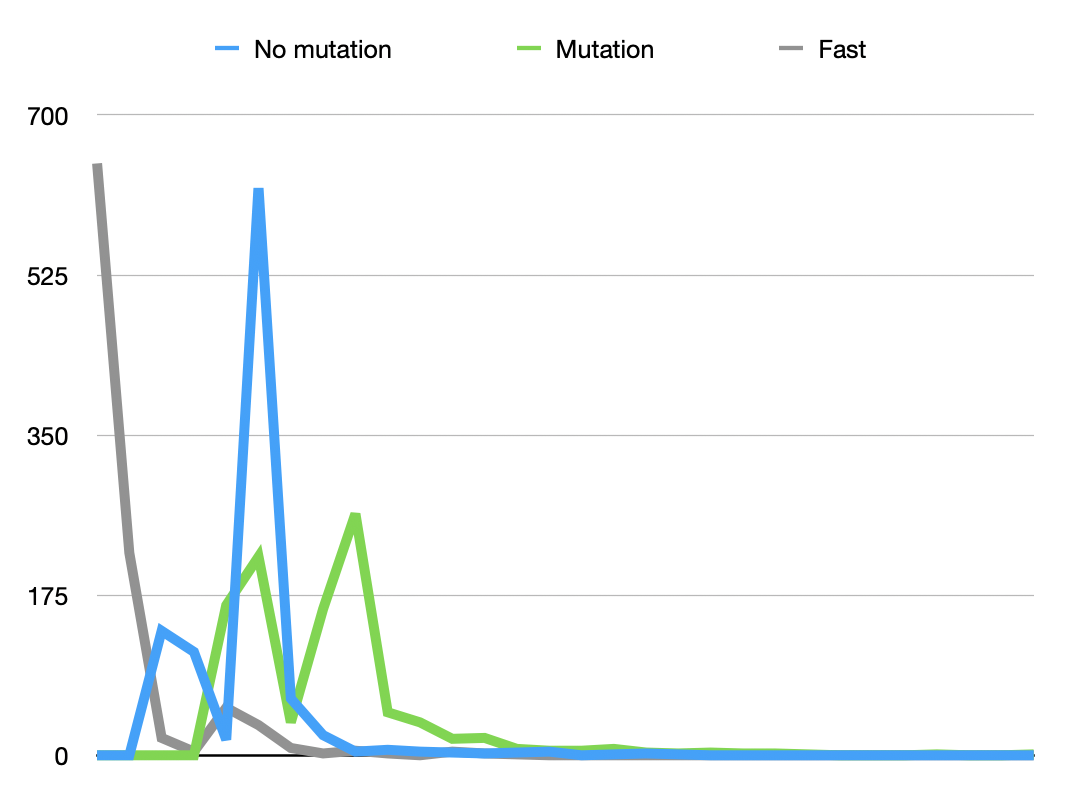
\includegraphics{Screenshot 2020-08-25 at 17.59.34.png} As you can see
the results aren't exactly as expected, both our \emph{average} and our
\emph{variance} is higher than without any optimisation. A result that
we definitely did not anticipate and goes against the belief that
founded our hypothesis.

One possible explanation is that scheme performs JIT compilation and
correctly identifies the hot-loop in our unoptimised example but is
unable to perform such optimisation with our mix of pure and mutating
code.

\hypertarget{fibonacci-without-startup-time-small-loop}{%
\paragraph{Fibonacci without startup time, small
loop}\label{fibonacci-without-startup-time-small-loop}}

In order to test the JIT hypothesis we are going to run the same test,
\emph{without} startup time but with a much smaller loop so that the
results are measured in milliseconds rather than seconds. This should be
enough to prevent the runtime from identifying the loop and performing
its optimisation.

In order to reduce the running time from seconds to milliseconds we
simply change the loop count from \texttt{8*10\^{}6} to
\texttt{8*10\^{}4} reducing it by two orders of magnitude reduces the
running time accordingly.

\begin{Shaded}
\begin{Highlighting}[]
\OperatorTok{../}\DataTypeTok{Idris2\_fib\_benchmark}\OperatorTok{/}\NormalTok{fibTestNoMutation}\OperatorTok{.}\NormalTok{idr,}
\FloatTok{0.007216185}\NormalTok{,}\FloatTok{0.008861124}\NormalTok{,}
\FloatTok{0.007520532116999987}\NormalTok{,}
\FloatTok{3.5827851856347296e{-}8}

\OperatorTok{../}\DataTypeTok{Idris2\_fib\_benchmark}\OperatorTok{/}\NormalTok{fibTest}\OperatorTok{.}\NormalTok{idr,}\FloatTok{0.006543267}\NormalTok{,}
\FloatTok{0.010942671}\NormalTok{,}
\FloatTok{0.006867369243000004}\NormalTok{,}
\FloatTok{5.3106313711037986e{-}8}

\OperatorTok{../}\DataTypeTok{Idris2\_fib\_benchmark}\OperatorTok{/}\NormalTok{fibTailRec}\OperatorTok{.}\NormalTok{idr,}
\FloatTok{0.006385357}\NormalTok{,}
\FloatTok{0.007625528}\NormalTok{,}
\FloatTok{0.006624731209000001}\NormalTok{,}
\FloatTok{2.4002041892751334e{-}8}

\NormalTok{[}\DecValTok{0}\NormalTok{, }\DecValTok{0}\NormalTok{, }\DecValTok{0}\NormalTok{, }\DecValTok{0}\NormalTok{, }\DecValTok{0}\NormalTok{, }\DecValTok{72}\NormalTok{, }\DecValTok{411}\NormalTok{, }\DecValTok{361}\NormalTok{, }\DecValTok{106}\NormalTok{, }\DecValTok{17}\NormalTok{, }\DecValTok{12}\NormalTok{, }\DecValTok{8}\NormalTok{, }\DecValTok{6}\NormalTok{, }\DecValTok{2}\NormalTok{, }\DecValTok{3}\NormalTok{, }\DecValTok{2}\NormalTok{, }
\DecValTok{0}\NormalTok{, }\DecValTok{0}\NormalTok{, }\DecValTok{0}\NormalTok{, }\DecValTok{0}\NormalTok{, }\DecValTok{0}\NormalTok{, }\DecValTok{0}\NormalTok{, }\DecValTok{0}\NormalTok{, }\DecValTok{0}\NormalTok{, }\DecValTok{0}\NormalTok{, }\DecValTok{0}\NormalTok{, }\DecValTok{0}\NormalTok{, }\DecValTok{0}\NormalTok{, }\DecValTok{0}\NormalTok{, }\DecValTok{0}\NormalTok{]}
\NormalTok{[}\DecValTok{0}\NormalTok{, }\DecValTok{95}\NormalTok{, }\DecValTok{493}\NormalTok{, }\DecValTok{288}\NormalTok{, }\DecValTok{83}\NormalTok{, }\DecValTok{13}\NormalTok{, }\DecValTok{9}\NormalTok{, }\DecValTok{10}\NormalTok{, }\DecValTok{3}\NormalTok{, }\DecValTok{0}\NormalTok{, }\DecValTok{3}\NormalTok{, }\DecValTok{1}\NormalTok{, }\DecValTok{0}\NormalTok{, }\DecValTok{0}\NormalTok{, }\DecValTok{0}\NormalTok{, }\DecValTok{0}\NormalTok{, }
\DecValTok{0}\NormalTok{, }\DecValTok{0}\NormalTok{, }\DecValTok{1}\NormalTok{, }\DecValTok{0}\NormalTok{, }\DecValTok{0}\NormalTok{, }\DecValTok{0}\NormalTok{, }\DecValTok{0}\NormalTok{, }\DecValTok{0}\NormalTok{, }\DecValTok{0}\NormalTok{, }\DecValTok{0}\NormalTok{, }\DecValTok{0}\NormalTok{, }\DecValTok{0}\NormalTok{, }\DecValTok{0}\NormalTok{, }\DecValTok{1}\NormalTok{]}
\NormalTok{[}\DecValTok{303}\NormalTok{, }\DecValTok{470}\NormalTok{, }\DecValTok{161}\NormalTok{, }\DecValTok{41}\NormalTok{, }\DecValTok{13}\NormalTok{, }\DecValTok{7}\NormalTok{, }\DecValTok{1}\NormalTok{, }\DecValTok{4}\NormalTok{, }\DecValTok{0}\NormalTok{, }\DecValTok{0}\NormalTok{, }\DecValTok{0}\NormalTok{, }\DecValTok{0}\NormalTok{, }\DecValTok{0}\NormalTok{, }\DecValTok{0}\NormalTok{, }\DecValTok{0}\NormalTok{, }\DecValTok{0}\NormalTok{, }
\DecValTok{0}\NormalTok{, }\DecValTok{0}\NormalTok{, }\DecValTok{0}\NormalTok{, }\DecValTok{0}\NormalTok{, }\DecValTok{0}\NormalTok{, }\DecValTok{0}\NormalTok{, }\DecValTok{0}\NormalTok{, }\DecValTok{0}\NormalTok{, }\DecValTok{0}\NormalTok{, }\DecValTok{0}\NormalTok{, }\DecValTok{0}\NormalTok{, }\DecValTok{0}\NormalTok{, }\DecValTok{0}\NormalTok{, }\DecValTok{0}\NormalTok{]}
\end{Highlighting}
\end{Shaded}

And indeed this data corroborates our hypothesis but does not confirm
that JIT was responsible for the previous performance results. However,
since this thesis is not about the intricacies of the scheme runtime we
are going to let the issue rest for now.

Those results showcase two things: That our optimisation works, and that
it is not significant enough to be strictly superior to other forms of
optimisations. Ideally the best way to test our optimisation would be to
write our own runtime which runs on \emph{bare metal} or some
approximation of it (WASM/LLVM) which would (probably) be even faster
than scheme. It would also give us more control over which optimisations
play nicely together (for example with JIT) and which ones are redundant
or even harmful to performance.

Idris2 has an alternative javascript backend, however, the javascript
code generation is unable to translate our programs into plain loops
free of recursion. Because of this, our benchmark exceeds the maximum
stack size and the program aborts. When the stack size is increased the
program segfaults. This could be solved with the use of trampolines in
the runtime, instead of plain recursion.

\hypertarget{mapping-a-list}{%
\subsubsection{Mapping a list}\label{mapping-a-list}}

In this exercise we are going to aggregate the result of our control and
our experimental run of \texttt{map}; which increments a list of number
and returns its size. We ran each program a 100 times using
\texttt{idris-bench}. As before we expect a negligible average speedup
but a significant decrease in variance.

\begin{Shaded}
\begin{Highlighting}[]
\OperatorTok{../}\NormalTok{map\_test}\OperatorTok{/}\FunctionTok{map}\OperatorTok{.}\NormalTok{idr,}
\FloatTok{8.73337e{-}4}\NormalTok{,}
\FloatTok{0.005067636}\NormalTok{,}
\FloatTok{0.0011461037300000004}\NormalTok{,}
\FloatTok{2.211481014400371e{-}7}

\OperatorTok{../}\NormalTok{map\_test\_mutate}\OperatorTok{/}\NormalTok{mapMutation}\OperatorTok{.}\NormalTok{idr,}
\FloatTok{5.23816e{-}4}\NormalTok{,}
\FloatTok{0.001308711}\NormalTok{,}
\FloatTok{6.850426700000001e{-}4}\NormalTok{,}
\FloatTok{1.9851180862141108e{-}8}

\NormalTok{[}\DecValTok{0}\NormalTok{, }\DecValTok{0}\NormalTok{, }\DecValTok{47}\NormalTok{, }\DecValTok{29}\NormalTok{, }\DecValTok{6}\NormalTok{, }\DecValTok{4}\NormalTok{, }\DecValTok{4}\NormalTok{, }\DecValTok{6}\NormalTok{, }\DecValTok{2}\NormalTok{, }\DecValTok{1}\NormalTok{, }\DecValTok{0}\NormalTok{, }\DecValTok{0}\NormalTok{, }\DecValTok{0}\NormalTok{, }\DecValTok{0}\NormalTok{, }\DecValTok{0}\NormalTok{, }\DecValTok{0}\NormalTok{, }\DecValTok{0}\NormalTok{, }
\DecValTok{0}\NormalTok{, }\DecValTok{0}\NormalTok{, }\DecValTok{0}\NormalTok{, }\DecValTok{0}\NormalTok{, }\DecValTok{0}\NormalTok{, }\DecValTok{0}\NormalTok{, }\DecValTok{0}\NormalTok{, }\DecValTok{0}\NormalTok{, }\DecValTok{0}\NormalTok{, }\DecValTok{0}\NormalTok{, }\DecValTok{0}\NormalTok{, }\DecValTok{0}\NormalTok{, }\DecValTok{1}\NormalTok{]}
\NormalTok{[}\DecValTok{63}\NormalTok{, }\DecValTok{26}\NormalTok{, }\DecValTok{5}\NormalTok{, }\DecValTok{5}\NormalTok{, }\DecValTok{0}\NormalTok{, }\DecValTok{1}\NormalTok{, }\DecValTok{0}\NormalTok{, }\DecValTok{0}\NormalTok{, }\DecValTok{0}\NormalTok{, }\DecValTok{0}\NormalTok{, }\DecValTok{0}\NormalTok{, }\DecValTok{0}\NormalTok{, }\DecValTok{0}\NormalTok{, }\DecValTok{0}\NormalTok{, }\DecValTok{0}\NormalTok{, }\DecValTok{0}\NormalTok{, }\DecValTok{0}\NormalTok{, }
\DecValTok{0}\NormalTok{, }\DecValTok{0}\NormalTok{, }\DecValTok{0}\NormalTok{, }\DecValTok{0}\NormalTok{, }\DecValTok{0}\NormalTok{, }\DecValTok{0}\NormalTok{, }\DecValTok{0}\NormalTok{, }\DecValTok{0}\NormalTok{, }\DecValTok{0}\NormalTok{, }\DecValTok{0}\NormalTok{, }\DecValTok{0}\NormalTok{, }\DecValTok{0}\NormalTok{, }\DecValTok{0}\NormalTok{]}
\end{Highlighting}
\end{Shaded}

This time our performance improvements are more noticeable in average
than before. Tough it might not be significant since it runs in tens of
microseconts

\hypertarget{sat-solver}{%
\subsection{Sat solver}\label{sat-solver}}

For this benchmark we didn't use \texttt{idris-bench} rather we compiled
two versions of \texttt{isat}
(\url{https://git.sr.ht/~cypheon/idris-minisat}), one with the inlining
optimisation, and one without. And ran each version 10 times on the same
input (in appendix) :

\begin{verbatim}
sat      | average            | variance
---------+--------------------+-----------------
normal   | 384008.545454545   | 337134927.872727
mutating | 371382.454545455   | 264041625.672727
\end{verbatim}

The results show an improvement of about 3.3\% in average which is
encouraging. This small improvement could be taken further by
implementing \emph{safe inlining by default} on every variable that is
linearly bound, since it does not hurt performance. And hope that the
inlined function will be subject to further optimisations after being
inlined.

\newpage

\hypertarget{future-work}{%
\section{Future work}\label{future-work}}

Work never ends and progress instils more progress, while a lot of
ground has been covered, exploring the forest of all knowledge not only
yields results, it uncovers new paths to explore. This section outlines
additional work that could be done in order to ease the use of linear
types as well as make use of them for additional functionality.

\hypertarget{enlarging-the-scope}{%
\subsection{Enlarging the scope}\label{enlarging-the-scope}}

The optimisation of section 6 only looks at the \emph{immediate} scope
of let bindings. Technically speaking there is nothing preventing our
optimisation from working with a more indirect scoping mechanism. Indeed
the following should trigger our optimisation

\begin{Shaded}
\begin{Highlighting}[]
\NormalTok{defaultVal }\OperatorTok{:} \DataTypeTok{MyData}
\NormalTok{defaultVal }\OtherTok{=} \DataTypeTok{MkDefault} \DecValTok{3}

\NormalTok{update }\OperatorTok{:}\NormalTok{ (}\DecValTok{1}\NormalTok{ rec }\OperatorTok{:} \DataTypeTok{MyData}\NormalTok{) }\OtherTok{{-}\textgreater{}} \DataTypeTok{MyData}
\NormalTok{update (}\DataTypeTok{MkDefault}\NormalTok{ n) }\OtherTok{=} \DataTypeTok{MkDefault}\NormalTok{ (}\DataTypeTok{S}\NormalTok{ n)}
\NormalTok{update (}\DataTypeTok{MkOther}\NormalTok{ n) }\OtherTok{=} \DataTypeTok{MkOther}\NormalTok{ (}\DataTypeTok{S}\NormalTok{ (}\DataTypeTok{S}\NormalTok{ n))}

\NormalTok{operate }\OperatorTok{:} \DataTypeTok{MyData}
\NormalTok{operate }\OtherTok{=} \KeywordTok{let} \DecValTok{1}\NormalTok{ def }\OtherTok{=}\NormalTok{ defaultVal}
              \DecValTok{1}\NormalTok{ newVal }\OtherTok{=}\NormalTok{ update def }\KeywordTok{in}
\NormalTok{              update newVal}
\end{Highlighting}
\end{Shaded}

But it will not because \texttt{defaultVal} is not a constructor, it's a
function call that returns itself a constructor.

One implementation strategy would be to wait for the compiler to inline
those definitions and then run our optimiser without further changes.

Another optimisation would be to follow references to see if they result
in plain data constructors and replace the entire call chain by the
constructor itself, and then run our optimisation.

While both those strategies are valid they incur a cost in terms of
complexity and compile time that may not be worth the effort in terms of
performance results. They could be hidden behind a -O3 flag, but that
kind of effort is probably better spend in making the ergonomics of
linear types more streamlined, which would help make those optimisations
more commonplace. Which is the topic of the next section

\hypertarget{making-linearity-easier-to-use}{%
\subsection{Making linearity easier to
use}\label{making-linearity-easier-to-use}}

There are multiple barriers that make linearity harder to use than one
might expect. They roughly end up in two buckets:

\begin{itemize}
\tightlist
\item
  I want to use linearity but I cannot
\item
  I have a linear variable and that's actually annoying
\end{itemize}

\hypertarget{not-linear-enough}{%
\subsubsection{Not linear enough}\label{not-linear-enough}}

The first one appears when the programmer tries to make thoughtful usage
of linear and erased annotation but finds that other parts of existing
libraries do not support linearity. The following program:

\begin{Shaded}
\begin{Highlighting}[]
\NormalTok{operate }\OperatorTok{:}\NormalTok{ (}\DecValTok{1}\NormalTok{ n }\OperatorTok{:} \DataTypeTok{Nat}\NormalTok{) }\OtherTok{{-}\textgreater{}}\NormalTok{ (}\DecValTok{1}\NormalTok{ m }\OperatorTok{:} \DataTypeTok{Nat}\NormalTok{) }\OtherTok{{-}\textgreater{}} \DataTypeTok{Int}
\NormalTok{operate n m }\OtherTok{=}\NormalTok{ n }\OperatorTok{+}\NormalTok{ m}
\end{Highlighting}
\end{Shaded}

Gives the error:

\begin{verbatim}
> Trying to use linear name n in non-linear context
\end{verbatim}

Because the \texttt{+} interface is defined as:

\begin{Shaded}
\begin{Highlighting}[]
\NormalTok{interface }\DataTypeTok{Num}\NormalTok{ ty }\KeywordTok{where}
\NormalTok{    (}\OperatorTok{+}\NormalTok{) }\OperatorTok{:}\NormalTok{ ty }\OtherTok{{-}\textgreater{}}\NormalTok{ ty }\OtherTok{{-}\textgreater{}}\NormalTok{ ty}
\end{Highlighting}
\end{Shaded}

Despite addition on \texttt{Nat} being defined linearly:

\begin{Shaded}
\begin{Highlighting}[]
\NormalTok{plus }\OperatorTok{:}\NormalTok{ (}\DecValTok{1}\NormalTok{ n }\OperatorTok{:} \DataTypeTok{Nat}\NormalTok{) }\OtherTok{{-}\textgreater{}}\NormalTok{ (}\DecValTok{1}\NormalTok{ m }\OperatorTok{:} \DataTypeTok{Nat}\NormalTok{) }\OtherTok{{-}\textgreater{}} \DataTypeTok{Nat}
\NormalTok{plus }\DataTypeTok{Z}\NormalTok{ m }\OtherTok{=}\NormalTok{ m}
\NormalTok{plus (}\DataTypeTok{S}\NormalTok{ n) m }\OtherTok{=} \DataTypeTok{S}\NormalTok{ (plus n m)}
\end{Highlighting}
\end{Shaded}

A similar problem occurs with interfaces

\begin{Shaded}
\begin{Highlighting}[]
\NormalTok{interface }\DataTypeTok{Monad}\NormalTok{ (}\DataTypeTok{Type} \OtherTok{{-}\textgreater{}} \DataTypeTok{Type}\NormalTok{) }\KeywordTok{where}
    \OperatorTok{...}

\KeywordTok{data} \DataTypeTok{MyData} \OperatorTok{:}\NormalTok{ (}\DecValTok{0}\NormalTok{ ty }\OperatorTok{:} \DataTypeTok{Type}\NormalTok{) }\OtherTok{{-}\textgreater{}} \DataTypeTok{Type} \KeywordTok{where}
    \OperatorTok{...}

\KeywordTok{instance} \DataTypeTok{Monad} \DataTypeTok{MyData} \KeywordTok{where}
    \OperatorTok{...}
\end{Highlighting}
\end{Shaded}

\begin{verbatim}
> Expected Type -> Type
> got (0 ty : Type) -> Type
\end{verbatim}

One way to solve those issues would be to have linearity polymorphism
and be able to abstract over linearity annotations. For example the map
function could be written as

\begin{Shaded}
\begin{Highlighting}[]
\FunctionTok{map} \OperatorTok{:} \KeywordTok{forall}\NormalTok{ l }\OperatorTok{.}\NormalTok{ ((l v }\OperatorTok{:}\NormalTok{ a) }\OtherTok{{-}\textgreater{}}\NormalTok{ b) }\OtherTok{{-}\textgreater{}}\NormalTok{ (l ls }\OperatorTok{:} \DataTypeTok{List}\NormalTok{ a) }\OtherTok{{-}\textgreater{}} \DataTypeTok{List}\NormalTok{ b}
\FunctionTok{map}\NormalTok{ f [] }\OtherTok{=}\NormalTok{ []}
\FunctionTok{map}\NormalTok{ f (}\OtherTok{x ::}\NormalTok{ xs) }\OtherTok{=}\NormalTok{ f}\OtherTok{ x ::} \FunctionTok{map}\NormalTok{ f xs}
\end{Highlighting}
\end{Shaded}

That is, the list is linearly consumed iff the higher order function is
linear. What it means for our interface problem is that it could be
rewritten as

\begin{Shaded}
\begin{Highlighting}[]
\NormalTok{interface }\KeywordTok{forall}\NormalTok{ l }\OperatorTok{.} \DataTypeTok{Functor}\NormalTok{ (m }\OperatorTok{:}\NormalTok{ (l \_ }\OperatorTok{:} \DataTypeTok{Type}\NormalTok{) }\OtherTok{{-}\textgreater{}} \DataTypeTok{Type}\NormalTok{) }\KeywordTok{where}
    \OperatorTok{...}
\NormalTok{interface }\KeywordTok{forall}\NormalTok{ l }\OperatorTok{.} \DataTypeTok{Functor}\NormalTok{ \{l\} m }\OtherTok{⇒} \DataTypeTok{Applicative}\NormalTok{ \{l\} m }\KeywordTok{where}
    \OperatorTok{...}
\NormalTok{interface }\KeywordTok{forall}\NormalTok{ l }\OperatorTok{.} \DataTypeTok{Applicative}\NormalTok{ \{l\} m }\OtherTok{⇒} \DataTypeTok{Monad}\NormalTok{ \{l\} m }\KeywordTok{where}
    \OperatorTok{...}
\end{Highlighting}
\end{Shaded}

A similar solution could be provided for \texttt{Num}

\begin{Shaded}
\begin{Highlighting}[]
\NormalTok{interface }\DataTypeTok{Num}\NormalTok{ ty }\KeywordTok{where}
\NormalTok{    (}\OperatorTok{+}\NormalTok{) }\OperatorTok{:} \KeywordTok{forall}\NormalTok{ l}\OperatorTok{.}\NormalTok{ (l n }\OperatorTok{:}\NormalTok{ ty) }\OtherTok{{-}\textgreater{}}\NormalTok{ (l m }\OperatorTok{:}\NormalTok{ ty) }\OtherTok{{-}\textgreater{}}\NormalTok{ ty}
\end{Highlighting}
\end{Shaded}

So that it can be used with both linear and non-linear variables.

\hypertarget{too-linear-now} linear in every aspect. We also
mentioned how this is a problem to implement basic functionality like
\texttt{drop} and \texttt{copy}, but those are artificial examples,
rarely does a programmer need to call \texttt{copy} or \texttt{drop} in
industrial applications. In the following example I will show how linear
types hold back programming and how QTT can fix it.

A common scenario when debugging effectful code is sprinkling around log
statements hoping that running the program will give insight into how
it's running.

\begin{Shaded}
\begin{Highlighting}[]
\KeywordTok{do}\NormalTok{ datas }\OtherTok{\textless{}{-}}\NormalTok{ getData arg1 arg2}
   \DataTypeTok{Just}\NormalTok{ success }\OtherTok{\textless{}{-}}\NormalTok{ trySomething datas (options}\OperatorTok{.}\NormalTok{memoized)}
     \OperatorTok{|}\NormalTok{ \_ }\OtherTok{⇒} \FunctionTok{pure} \OperatorTok{$}\NormalTok{ returnError }\StringTok{"couldn\textquotesingle{}t make it work"}
   \KeywordTok{case} \OperatorTok{!}\NormalTok{(check\_timestamp success) }\KeywordTok{of}
      \DataTypeTok{Safe}\NormalTok{ t v }\OtherTok{⇒}\NormalTok{ functionCall t v}
      \DataTypeTok{Unsafe}\NormalTok{ t }\OtherTok{⇒}\NormalTok{ trySomethingElse t}
      \DataTypeTok{UnSynchronized}\NormalTok{ v }\OtherTok{⇒}\NormalTok{ functionCall }\DecValTok{0}\NormalTok{ v }
      \DataTypeTok{Invalid} \OtherTok{⇒} \FunctionTok{pure} \OperatorTok{$}\NormalTok{ returnError }\StringTok{"failed to check"}
\end{Highlighting}
\end{Shaded}

Assuming everything is linear, there is no possible way to add a new
print statement without getting a linearity error:

\begin{Shaded}
\begin{Highlighting}[]
\KeywordTok{do}\NormalTok{ datas }\OtherTok{\textless{}{-}}\NormalTok{ getData arg1 arg2}
   \DataTypeTok{Just}\NormalTok{ success }\OtherTok{\textless{}{-}}\NormalTok{ trySomething datas (options}\OperatorTok{.}\NormalTok{memoized)}
     \OperatorTok{|}\NormalTok{ \_ }\OtherTok{⇒} \FunctionTok{pure} \OperatorTok{$}\NormalTok{ returnError }\StringTok{"couldn\textquotesingle{}t make it work"}
   \FunctionTok{putStrLn} \OperatorTok{$} \FunctionTok{show}\NormalTok{ success }
   \CommentTok{{-}{-}                 ▲}
   \CommentTok{{-}{-}                 └── One use here}
   \CommentTok{{-}{-}   And one use there ──┐}
   \CommentTok{{-}{-}                       ▼}
   \KeywordTok{case} \OperatorTok{!}\NormalTok{(check\_timestamp success) }\KeywordTok{of}
      \DataTypeTok{Safe}\NormalTok{ t v }\OtherTok{⇒}\NormalTok{ functionCall t v}
      \DataTypeTok{Unsafe}\NormalTok{ t }\OtherTok{⇒}\NormalTok{ trySomethingElse t}
      \DataTypeTok{UnSynchronized}\NormalTok{ v }\OtherTok{⇒}\NormalTok{ functionCall }\DecValTok{0}\NormalTok{ v }
      \DataTypeTok{Invalid} \OtherTok{⇒} \FunctionTok{pure} \OperatorTok{$}\NormalTok{ returnError }\StringTok{"failed to check"}
\end{Highlighting}
\end{Shaded}

We've already mentioned how borrowing and quantitative types would help
us implement reference counting. In this case they have a more
user-facing property, allowing programming updates without using
unrestricted variables, which loses us the benefits of quantitative
types. Using \emph{precise usage} as our quantity would result in the
following program:

\begin{Shaded}
\begin{Highlighting}[]
\KeywordTok{do}\NormalTok{ datas }\OtherTok{\textless{}{-}}\NormalTok{ getData arg1 arg2}
   \DecValTok{2}\NormalTok{ (}\DataTypeTok{Just}\NormalTok{ success) }\OtherTok{\textless{}{-}}\NormalTok{ trySomething datas (options}\OperatorTok{.}\NormalTok{memoized)}
     \OperatorTok{|}\NormalTok{ \_ }\OtherTok{⇒} \FunctionTok{pure} \OperatorTok{$}\NormalTok{ returnError }\StringTok{"couldn\textquotesingle{}t make it work"}
   \FunctionTok{putStrLn} \OperatorTok{$} \FunctionTok{show}\NormalTok{ success}
   \KeywordTok{case} \OperatorTok{!}\NormalTok{(check\_timestamp success) }\KeywordTok{of}
\NormalTok{       …}
\end{Highlighting}
\end{Shaded}

Which will allow \texttt{success} to be bound with linearity \texttt{2}
and therefore used twice. We can also allow \emph{borrowing} of
read-only variables to fix the same problem:

\begin{Shaded}
\begin{Highlighting}[]
\KeywordTok{do}\NormalTok{ datas }\OtherTok{\textless{}{-}}\NormalTok{ getData arg1 arg2}
   \DataTypeTok{Just}\NormalTok{ success }\OtherTok{\textless{}{-}}\NormalTok{ trySomething datas (options}\OperatorTok{.}\NormalTok{memoized)}
     \OperatorTok{|}\NormalTok{ \_ }\OtherTok{⇒} \FunctionTok{pure} \OperatorTok{$}\NormalTok{ returnError }\StringTok{"couldn\textquotesingle{}t make it work"}
   \FunctionTok{putStrLn} \OperatorTok{$} \FunctionTok{show} \OperatorTok{\&}\NormalTok{success }\CommentTok{{-}{-} this doesn\textquotesingle{}t count as a use}
   \KeywordTok{case} \OperatorTok{!}\NormalTok{(check\_timestamp success) }\KeywordTok{of}
\end{Highlighting}
\end{Shaded}

We've seen that read-only variables have been a topic for linearly typed
system with \emph{Linear Types can change the
world}\cite{linear_types_update}, where linear read-only variables are
allowed within some restriction on their scope. It would be interesting
to implement a similar set of rules, adapted for QTT, that allows
multiple use of linear types as long as they are read-only and our
\texttt{\%mutating} implementation to differentiate between read-only
and mutating functions.

\newpage

\hypertarget{conclusion}{%
\section{Conclusion}\label{conclusion}}

I have learned a lot during this master project. Not only about linear
types, quantitative types, graded modal types, containers, categories,
optimisation techniques, benchmarking, program safety, compiler design
and implementation, etc.

But I also learned about myself and how I best approach research topics.
Research is not an activity to carry out alone, it is not a mindless
job, and it is not limited to the ivory tower that is higher education.
I learned that I do my best research work when I explore the paths that
opens in the forest of knowledge after clearing one of them. I would
never have understood graded modalities if I wasn't distracted by
semirings. I would never have understood semirings if I wasn't
frustrated porting some code to Idris2 and noticing the limitations of
\texttt{0}, \texttt{1} and \texttt{ω}. I would have never started
porting code to Idris2 if I wasn't looking for an escape from writing
test for my performance improvements.

While this behaviour is dangerous, in that it can result in nothing of
value produced, it also taught me the importance of having a strong and
reliable support group. Friends, both in research and otherwise, focus
the mind, which results in a more focused work. Finally, research is not
something one can \emph{tune out of}, thoughts linger, ideas sprawl out
of control and new connections are drawn during every event of daily
life. I have discovered that sharing my research through teaching has
been an extremely effective mean to contextualise my work and to put
boundaries between personal and research life.

Quantitative types, just like me, still have a long way to go. The work
displayed here is only a minuscule sliver of what can be done, and needs
to be done, for them to become commercially significant. In line with
the two main topics of this thesis, I think the areas quantitative types
need to improve are ergonomics and performance. They are two pain points
that functional programming has failed to fix, while other programming
language have been successful basing their entire value proposition upon
them (Rust, Javascript, Python, etc).

Ergonomics have made huge strides forward with interactive development
environment like we find in Idris, Agda or Coq. But their gimmicks
cannot sustain the behemoth of features that commercially successful
programming languages showcase. Linear types won't turn the balance
around, but they will help in some important aspects: ensuring APIs
contracts and protocols are respected, showing those information in the
type, and therefore in the documentation, help the compiler generate
more helpful error messages, and help guide new users navigate complex
programs by being explicit about usage rules that were left unwritten
before.

Until the recent development in resource tracking technologies, it
wasn't clear how the concept of performance could be approached and
studied in functional programming. We did not have a way to get a hold
of it. But just like we did not have a way to get a hold onto
side-effect until monads, I strongly suspect quantitative types will
allow us to turn performance from an abstract concept into a concrete
term in a programming language, just like \texttt{IO} became a concrete
term in functional programming languages.

I hope you enjoyed this report on linear and quantitative types as much
as I did writing it. I wish I explored the paths of knowledge that I
discovered with more depth. Yet I am satisfied with the result of this
year of exploration. I come out of it with a strong intuition about
quantitative types, how to use them and how to improve them. I strongly
believe this thesis, as the first detailed exploration of quantitative
types used in practice with dependent types, will be the start of a
series of great discoveries.

\newpage

\hypertarget{appendices-glossary-and-definitions}{%
\section{Appendices: Glossary and
definitions}\label{appendices-glossary-and-definitions}}

While the initial list of fancy words in the introduction is nice it
suffers from being superficial and therefore incomplete. These are more
details definitions using examples and imagery

\hypertarget{affine-types}{%
\subsection{Affine types}\label{affine-types}}

Affine types describe values that can be used at most 0 times, at most 1
times or at most infinitely many times (aka no restrictions)

\hypertarget{co-monad-comonad}{%
\subsection{Co-monad / Comonad}\label{co-monad-comonad}}

A mathematical structure that allows to encapsulate \emph{access to a
context}. For example \texttt{List} is a Comonad because it allows us to
work in a context were the value we manipulate is one out of many
available to us, those other values available to us are the other values
of the list.

\hypertarget{indexed-type}{%
\subsection{Indexed type}\label{indexed-type}}

A \emph{type parameter} that changes with the values that inhabit the
type. For example \texttt{{[}"a",\ "b",\ "c"{]}\ :\ Vect\ 3\ String} has
index \texttt{3} and a type parameter \texttt{String}, because it has
\texttt{3} elements and the elements are Strings. If the value was
\texttt{{[}\textasciigrave{}"a",\ “b”{]}} then the type would become
\texttt{Vect\ 2\ String}, the index would change from \texttt{3} to
\texttt{2}, but the type parameter would stay as \texttt{String}.

\hypertarget{implicit-argument}{%
\subsection{Implicit argument}\label{implicit-argument}}

An implicit argument is one that needs not be filled out at call site
because the compiler will fill in the argument for you. In the type
signature:
\texttt{length\ :\ \{n\ :\ Nat\}\ -\textgreater{}\ Vect\ n\ a\ -\textgreater{}\ Nat}
the argument \texttt{n} is implicit.

\hypertarget{lattice}{%
\subsection{Lattice}\label{lattice}}

A mathematical structure that relates values to one another in a way
that doesn't allow arbitrary comparison between two arbitrary values.
Here is a pretty picture of one:

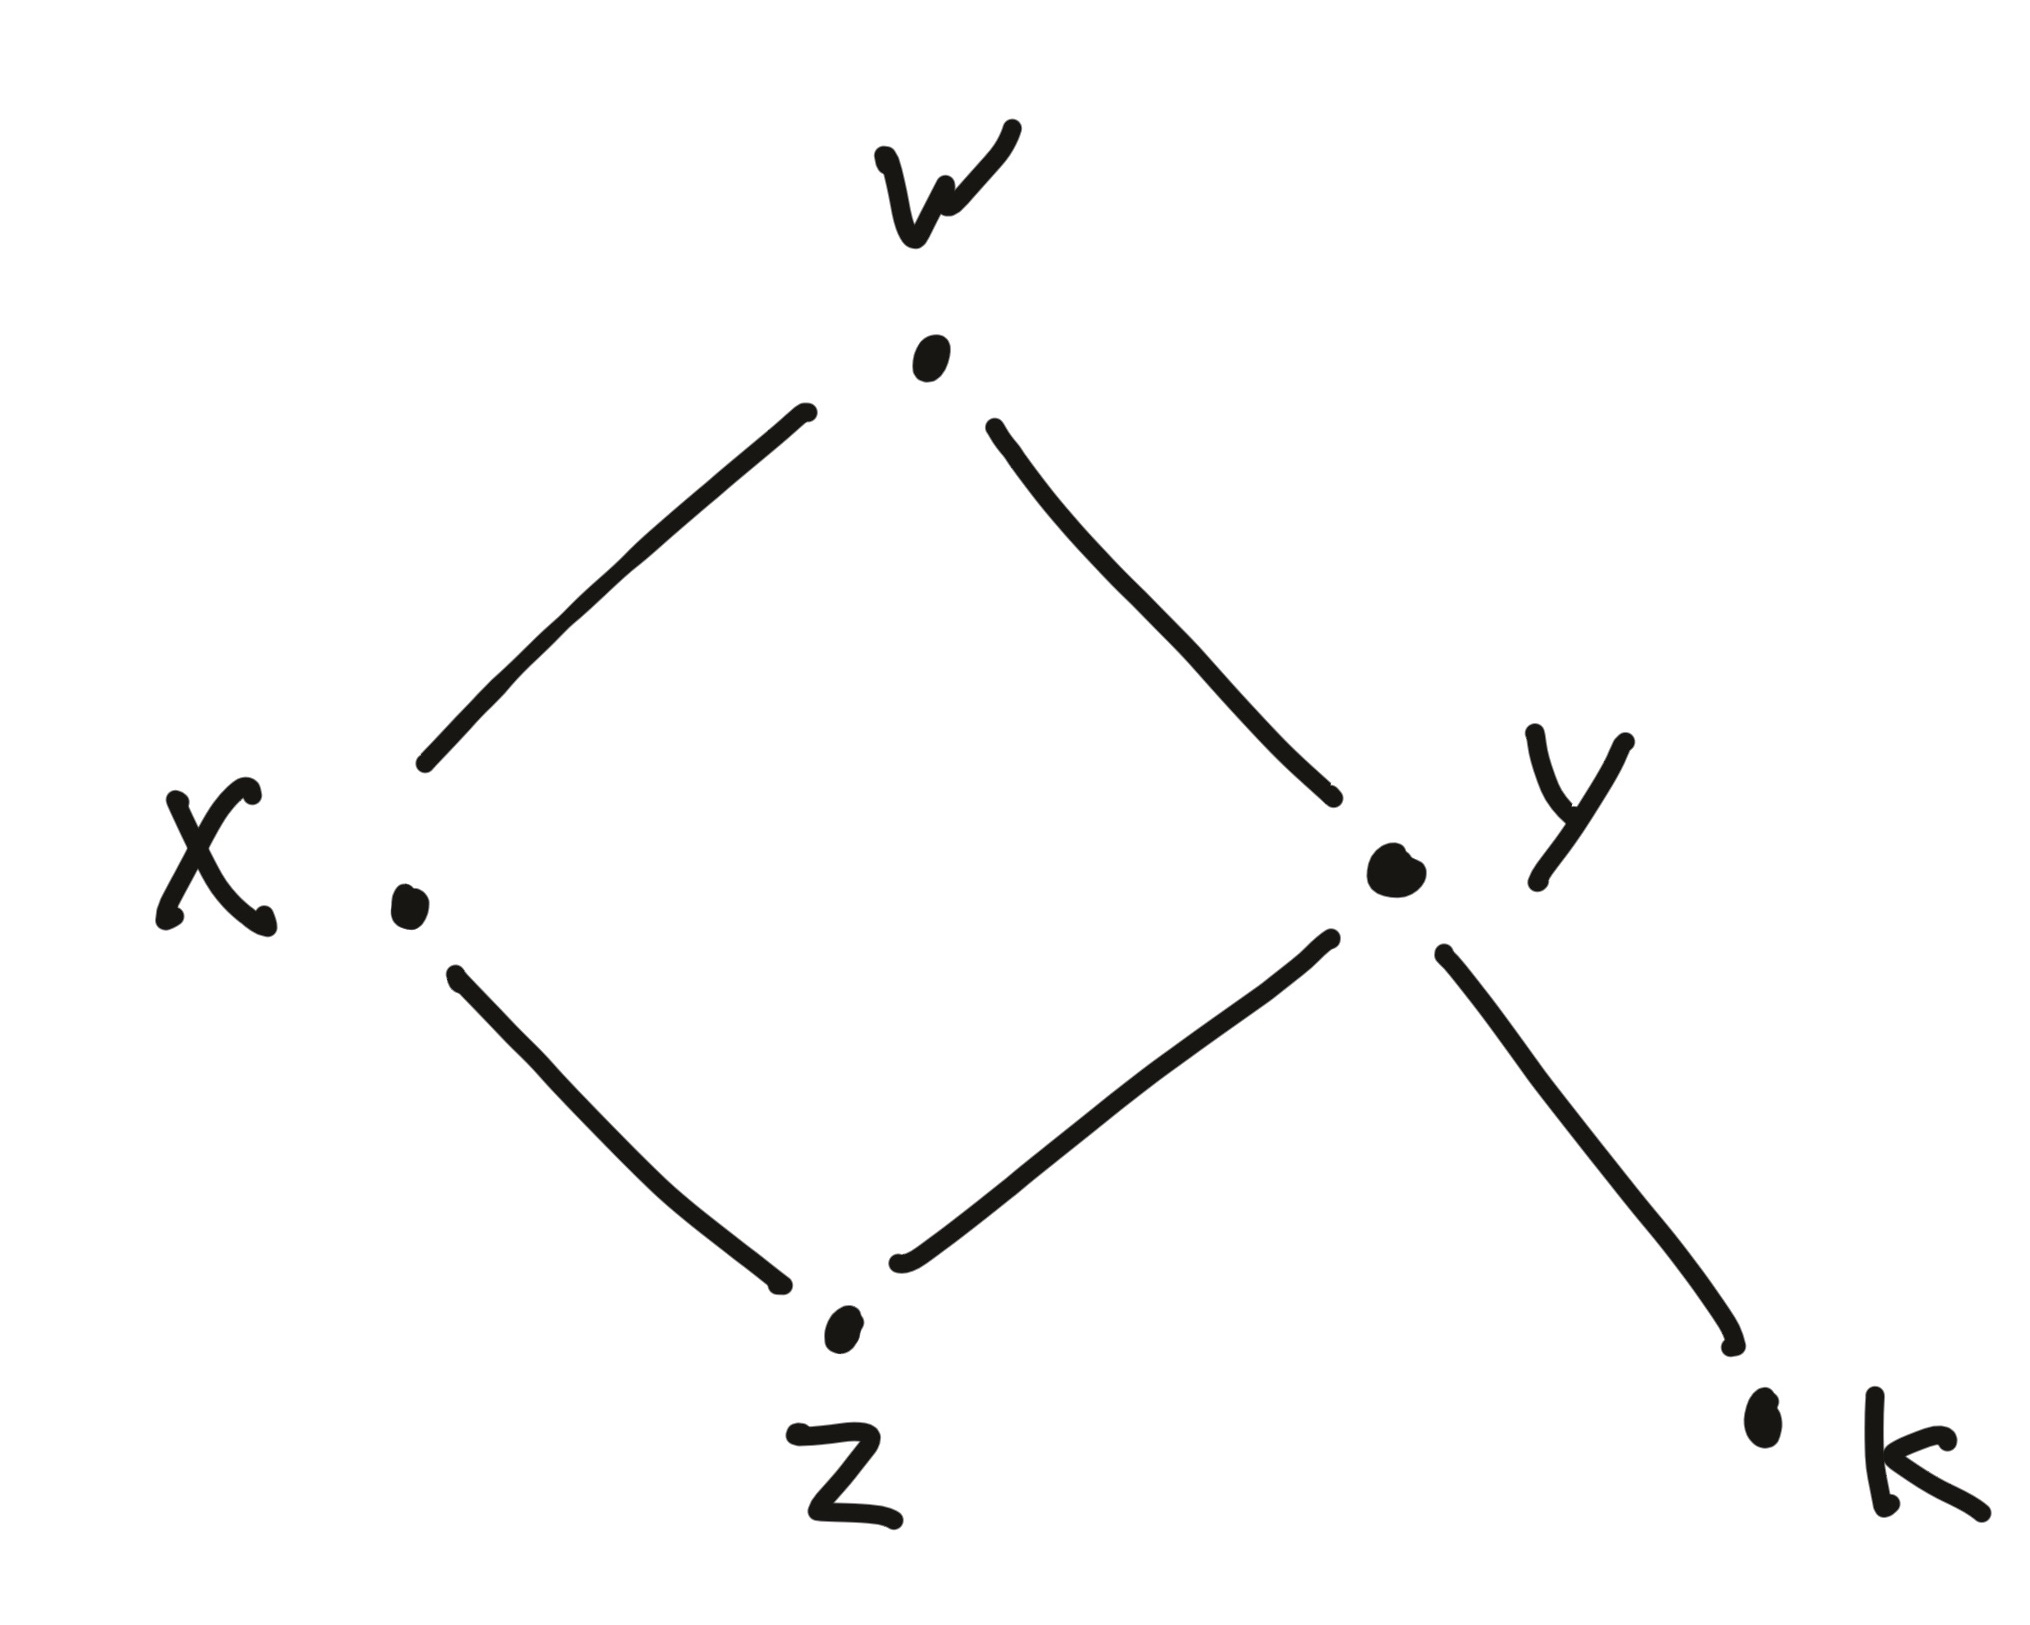
\includegraphics{lattice.jpg}

As you can see we can't really tell what's going on between X and Y,
they aren't related directly, but we can tell that they are both smaller
than W and greater than Z

\hypertarget{linear-types-1}{%
\subsection{Linear types}\label{linear-types-1}}

Linear types describe values that can be used exactly 0 times, exactly 1
time or have no restriction put on them

\hypertarget{linearity-multiplicity}{%
\subsection{Linearity / Multiplicity}\label{linearity-multiplicity}}

Used interchangeably most of the time. They refer the the number of
times a variable is expected to be used. Technically there is a slight
difference between those three terms:

\begin{itemize}
\tightlist
\item
  Linearity refers to variables that can be used exactly once
\item
  Multiplicity refers to the number of times a variable can be used. Not
  only exactly once, and not only just numbers.
\end{itemize}

\hypertarget{monad}{%
\subsection{Monad}\label{monad}}

A mathematical structure that allows to encapsulate \emph{change in a
context}. For example \texttt{Maybe} is a Monad because it creates a
context in which the values we are manipulating might be absent.
Formally, a monad is a triple between an indexed set \(X_i\) a
\texttt{bind} operation \(X_a \to (a \to X_b) \to X_b\) and a
\texttt{pure} operation \(1 \to X_a\)

\hypertarget{pattern-matching-1}{%
\subsection{Pattern matching}\label{pattern-matching-1}}

Pattern matching consists in destructuring a value into its constituent
parts in order to access them or understand what kind of value we are
dealing with.

\hypertarget{semiring}{%
\subsection{Semiring}\label{semiring}}

A mathematical structure that requires its values to be combined with
\texttt{+} and \texttt{*} in the ways you expect from natural numbers

\hypertarget{syntax-1}{%
\subsection{Syntax}\label{syntax-1}}

The structure of some piece of information, usual in the form of
\emph{text}. Syntax itself does not convey any meaning. Imagine this
piece of data

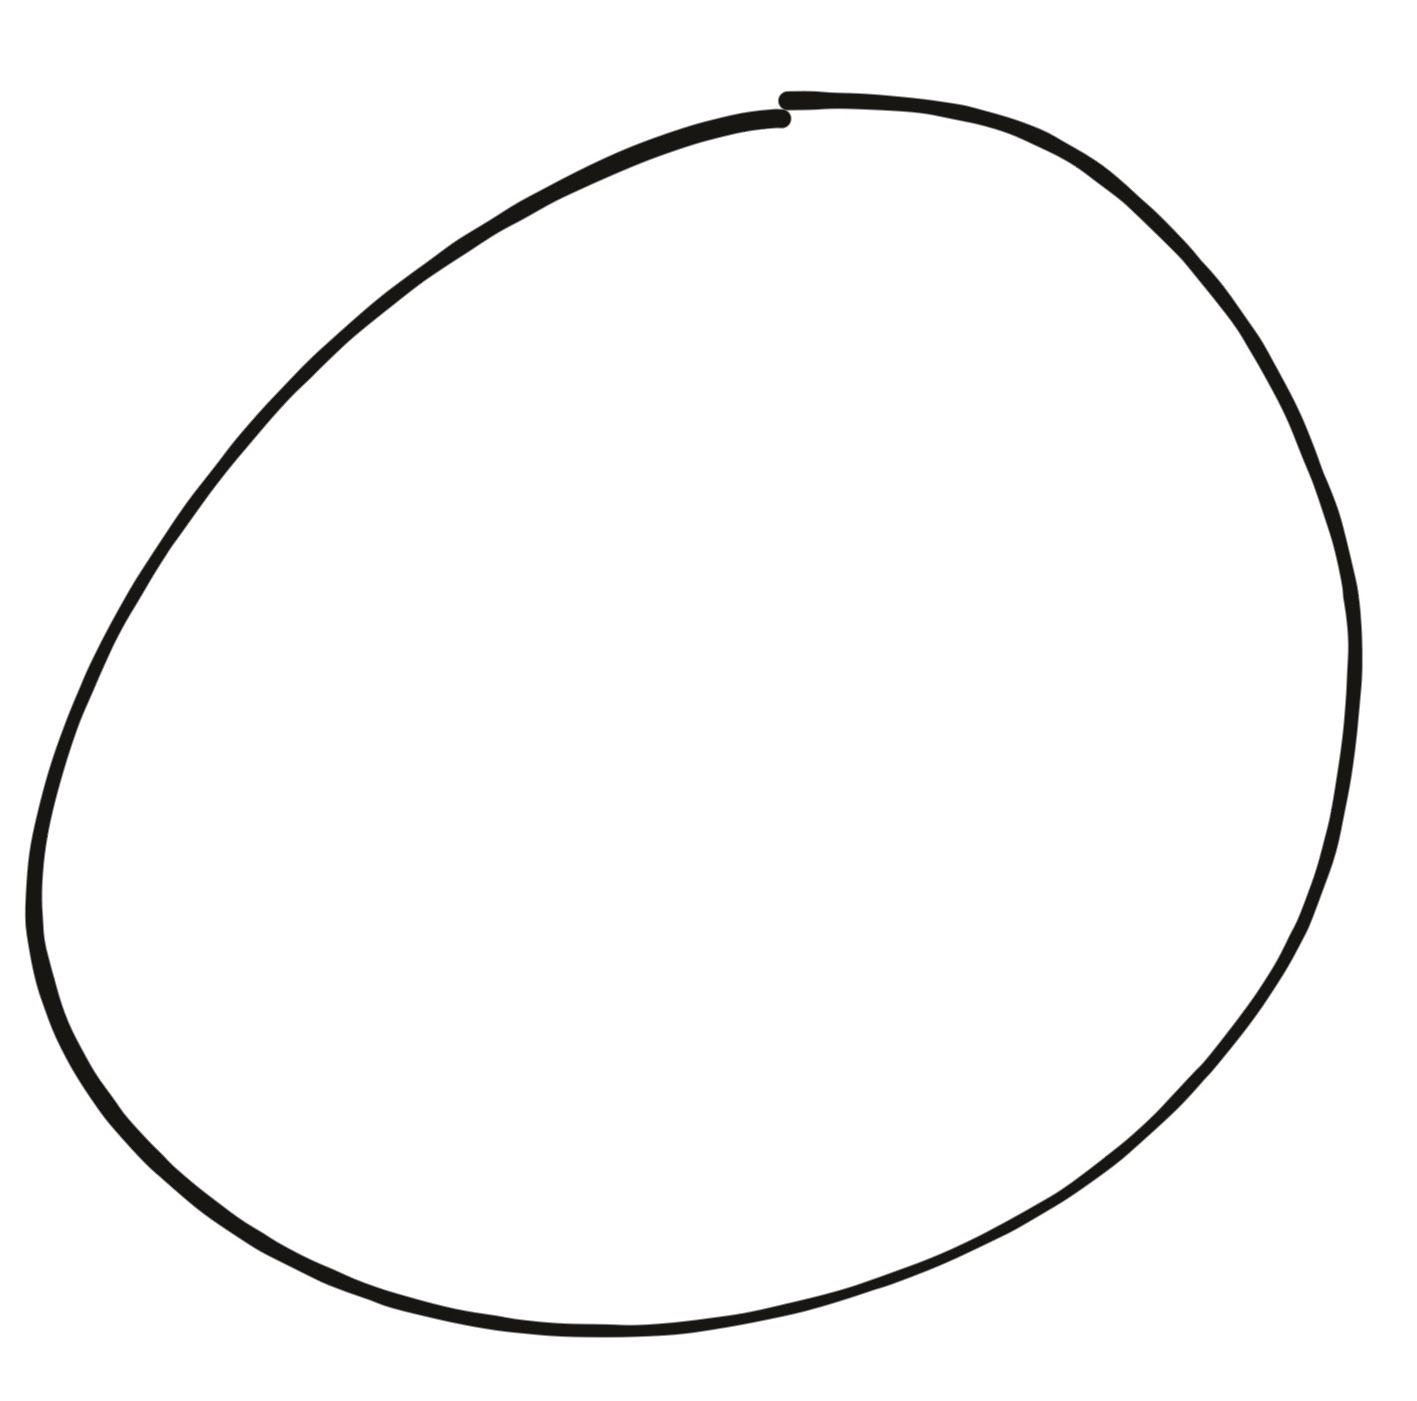
\includegraphics{Zero.jpg}

We can define a syntactic rules that allow us to express this circle,
here is one: all shapes that you can draw without lifting your pen or
making angles. From this definition lots of values are allowed,
including \textbar, -, O but not + for example because there is a 90º
angle between two bars. Is it supposed to be the letter ``O'', the
number ``0'' the silouhette of a planet? the back of the head of a stick
figure from the back?

\hypertarget{semantics-1}{%
\subsection{Semantics}\label{semantics-1}}

The meaning associated to a piece of data, most often related to syntax.
From the \emph{syntax} definition if we have:

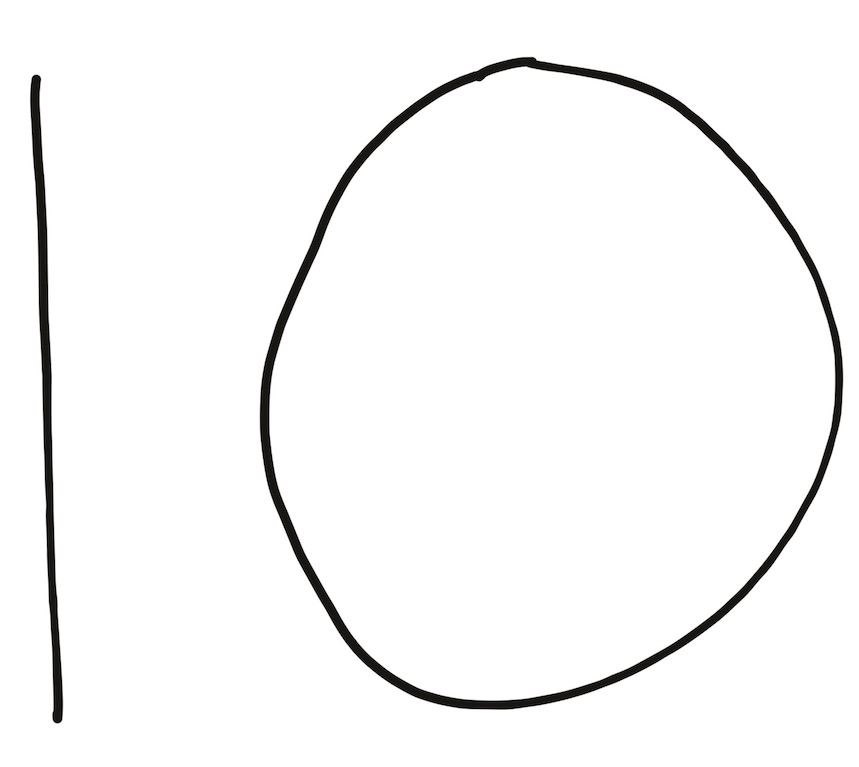
\includegraphics{ten.jpg}

We can deduce that the circle means ``the second digit of the number
10'' which is the number ``0''. We were able to infer semantics from
context. Similary in this picture:


\includegraphics{Smiley smol.jpeg}

We can deduce that the meaning of the circle was to represent the head
of a stick figure from the front.

\hypertarget{type-system-1}{%
\subsection{Type system}\label{type-system-1}}

Set of rules the types in a program have to follow in order to be
accepted by the compiler. The goal of the type-system is to catch some
classes of errors while helping the programmer reach their goal more
easily.

\hypertarget{type-theory}{%
\subsection{Type theory}\label{type-theory}}

\emph{Type theory} is the abstract study of type systems, most often in
the context of pure, mathematical, logic. When we say ``a Type Theory''
we mean a specific set of logical rules that can be implemented into a
\emph{Type System}.

\bibliography{bibliography} 
\bibliographystyle{ieeetr}

\hypertarget{appendix}{%
\section{Appendix}\label{appendix}}

\hypertarget{sat-solver-benchmark-input}{%
\subsection{Sat solver benchmark
input}\label{sat-solver-benchmark-input}}

\begin{verbatim}
c FILE: aim-50-1_6-yes1-4.cnf
c
c SOURCE: Kazuo Iwama, Eiji Miyano (miyano@cscu.kyushu-u.ac.jp),
c          and Yuichi Asahiro
c
c DESCRIPTION: Artifical instances from generator by source.  Generators
c              and more information in sat/contributed/iwama.
c
c NOTE: Satisfiable
c
p cnf 50 80
16 17 30 0
-17 22 30 0
-17 -22 30 0
16 -30 47 0
16 -30 -47 0
-16 -21 31 0
-16 -21 -31 0
-16 21 -28 0
-13 21 28 0
13 -16 18 0
13 -18 -38 0
13 -18 -31 0
31 38 44 0
-8 31 -44 0
8 -12 -44 0
8 12 -27 0
12 27 40 0
-4 27 -40 0
12 23 -40 0
-3 4 -23 0
3 -23 -49 0
3 -13 -49 0
-23 -26 49 0
12 -34 49 0
-12 26 -34 0
19 34 36 0
-19 26 36 0
-30 34 -36 0
24 34 -36 0
-24 -36 43 0
6 42 -43 0
-24 42 -43 0
-5 -24 -42 0
5 20 -42 0
5 -7 -20 0
4 7 10 0
-4 10 -20 0
7 -10 -41 0
-10 41 46 0
-33 41 -46 0
33 -37 -46 0
32 33 37 0
6 -32 37 0
-6 25 -32 0
-6 -25 -48 0
-9 28 48 0
-9 -25 -28 0
19 -25 48 0
2 9 -19 0
-2 -19 35 0
-2 22 -35 0
-22 -35 50 0
-17 -35 -50 0
-29 -35 -50 0
-1 29 -50 0
1 11 29 0
-11 17 -45 0
-11 39 45 0
-26 39 45 0
-3 -26 45 0
-11 15 -39 0
14 -15 -39 0
14 -15 -45 0
14 -15 -27 0
-14 -15 47 0
17 17 40 0
1 -29 -31 0
-7 32 38 0
-14 -33 -47 0
-1 2 -8 0
35 43 44 0
21 21 24 0
20 29 -48 0
23 35 -37 0
2 18 -33 0
15 25 -45 0
9 14 -38 0
-5 11 50 0
-3 -13 46 0
-13 -41 43 0
\end{verbatim}

\hypertarget{sat-solver-benchmark-output}{%
\subsection{Sat solver benchmark
output}\label{sat-solver-benchmark-output}}

\begin{verbatim}
,,,,,,,,,,,,average,variance,,,,,,,,,
normal,5m 51s 878ms,5m 52s 27ms,6m 29s 173ms,6m 35s 147ms,6m 34s 151ms,6m 35s 888ms,6m 36s 815ms,6m 35s 960ms,6m 33s 967ms,6m 34s 964ms,6m 4s 124ms,6m 24s 9ms,,,,,,,,,,
mutat,6m 27s 894ms,6m 21s 214ms,6m 10s 131ms,6m 27s 206ms,6m 4s 71ms,6m 25s 495ms,6m 27s 899ms,6m 13s 771ms,5m 51s 541ms,5m 47s 685ms,5m 48s 300ms,6m 11s 382ms,,,,,,,,,,
normal milisec,351878,352027,389173,395147,394151,395888,396815,395960,393967,394964,364124,384008.545454545,337134927.872727,,,,,,,,,
mutating milisec,387894,381214,370131,387206,364071,385495,387899,373771,351541,347685,348300,371382.454545455,264041625.672727,,,,,,,,,
normal milisec * 10^5,3.51878,3.52027,3.89173,3.95147,3.94151,3.95888,3.96815,3.9596,3.93967,3.94964,3.64124,3.84008545454545,0.0337134927872727,,,,,,,,,
mutating milisec * 10⁵,3.87894,3.81214,3.70131,3.87206,3.64071,3.85495,3.87899,3.73771,3.51541,3.47685,3.483,3.71382454545455,0.0264041625672727,,,,,,,,,
\end{verbatim}

\end{document}
